\documentclass{ConfigurationFiles/PoliMi3i_thesis}


% CONFIGURATIONS
\usepackage{parskip} % For paragraph layout
\usepackage{setspace} % For using single or double spacing
\usepackage{emptypage} % To insert empty pages
\usepackage{multicol} % To write in multiple columns (executive summary)
\setlength\columnsep{15pt} % Column separation in executive summary
\setlength\parindent{0pt} % Indentation
\raggedbottom
\usepackage{multirow}

% PACKAGES FOR TITLES
\usepackage{titlesec}
% \titlespacing{\section}{left spacing}{before spacing}{after spacing}
\titlespacing{\section}{0pt}{3.3ex}{2ex}
\titlespacing{\subsection}{0pt}{3.3ex}{1.65ex}
\titlespacing{\subsubsection}{0pt}{3.3ex}{1ex}
\usepackage{color}

% PACKAGES FOR LANGUAGE AND FONT
\usepackage[english]{babel} % The document is in English  
\usepackage[utf8]{inputenc} % UTF8 encoding
\usepackage[T1]{fontenc} % Font encoding
\usepackage[11pt]{moresize} % Big fonts

% PACKAGES FOR IMAGES
\usepackage{graphicx}
\usepackage{transparent} % Enables transparent images
\usepackage{eso-pic} % For the background picture on the title page
\usepackage{subfig} % Numbered and caption subfigures using \subfloat.
\usepackage{tikz} % A package for high-quality hand-made figures.
\usetikzlibrary{}
\graphicspath{{./images/}} % Directory of the images
\usepackage{amsthm} % Coloured "Theorem"
\usepackage{thmtools}
\usepackage{xcolor}
\usepackage{float}

% STANDARD MATH PACKAGES
\usepackage{amsmath}
\usepackage{amssymb}
\usepackage{amsfonts}
\usepackage{bm}
\usepackage[overload]{empheq} % For braced-style systems of equations.
\usepackage{fix-cm} % To override original LaTeX restrictions on sizes

% PACKAGES FOR TABLES
\usepackage{tabularx}
\usepackage{longtable} % Tables that can span several pages
\usepackage{colortbl}

% PACKAGES FOR ALGORITHMS (PSEUDO-CODE)
\usepackage{algorithm}
\usepackage{algorithmic}


% PACKAGES FOR REFERENCES & BIBLIOGRAPHY
\usepackage[
    colorlinks=true,
    linkcolor=black,
    anchorcolor=black,
    citecolor=black,
    filecolor=black,
    menucolor=black,
    runcolor=black,
    urlcolor=black
]{hyperref} % Adds clickable links at references
\usepackage{cleveref}
\usepackage[square, numbers, sort&compress]{natbib} % Square brackets, citing references with numbers, citations sorted by appearance in the text and compressed
\bibliographystyle{abbrvnat} % You may use a different style adapted to your field

% OTHER PACKAGES
\usepackage[normalem]{ulem}
\usepackage{verbatim}
\usepackage[super]{nth}
\usepackage{pdfpages} % To include a pdf file
\usepackage{afterpage}
\usepackage{lipsum} % DUMMY PACKAGE
\usepackage{fancyhdr}
\usepackage{wasysym} % For the headers
\usepackage{rotating}
\usepackage{listings}
\usepackage{hyperref}
\usepackage{enumitem}
%%
% Alloy language definition for using with the listings package.
%
% 2017, Daniel Andrade
% BSD 3-Clause License
%%
\lstdefinelanguage{alloy}{
    morekeywords={
        module, open, as,
        private, abstract, sig, extends, in,
        lone, some, one, disj,
        fact, pred, fun, assert,
        run, check,
        for, but, exactly,
        this, not, implies, else, let,
        not, no, set, all, sum,
        iff, or, Int, and,
        none, univ, iden
    },
    sensitive=true,
    morecomment=[l]{//},
    morecomment=[l]{--},
    morecomment=[s]{/*}{*/},
    morestring=[b]{"},
%literate={->}{$\rightarrow$}1
% replacing characters can cause problems when copying from PDF to editor
}[keywords,comments,strings]

\fancyhf{}

% Input of configuration file. Do not change config.tex file unless you really know what you are doing. 
% Define blue color typical of polimi
\definecolor{bluepoli}{cmyk}{0.4,0.1,0,0.4}

% Custom theorem environments
\declaretheoremstyle[
    headfont=\color{bluepoli}\normalfont\bfseries,
    bodyfont=\color{black}\normalfont\itshape,
]{colored}

% Set-up caption colors
\captionsetup[figure]{labelfont={color=bluepoli}} % Set colour of the captions
\captionsetup[table]{labelfont={color=bluepoli}} % Set colour of the captions
\captionsetup[algorithm]{labelfont={color=bluepoli}} % Set colour of the captions

\theoremstyle{colored}
\newtheorem{theorem}{Theorem}[chapter]
\newtheorem{proposition}{Proposition}[chapter]

% Enhances the features of the standard "table" and "tabular" environments.
\newcommand\T{\rule{0pt}{2.6ex}}
\newcommand\B{\rule[-1.2ex]{0pt}{0pt}}

% Pseudo-code algorithm descriptions.
\newcounter{algsubstate}
\renewcommand{\thealgsubstate}{\alph{algsubstate}}
\newenvironment{algsubstates}
{\setcounter{algsubstate}{0}%
\renewcommand{\STATE}{%
    \stepcounter{algsubstate}%
    \Statex {\small\thealgsubstate:}\space}}
{}

% New font size
\newcommand\numfontsize{\@setfontsize\Huge{200}{60}}

% Title format: chapter
\titleformat{\chapter}[hang]{
    \fontsize{50}{20}\selectfont\bfseries\filright}{\textcolor{bluepoli} \thechapter\hsp\hspace{2mm}\textcolor{bluepoli}{|   }\hsp}{0pt}{\huge\bfseries \textcolor{bluepoli}
}

% Title format: section
\titleformat{\section}
{\color{bluepoli}\normalfont\Large\bfseries}
{\color{bluepoli}\thesection.}{1em}{}

% Title format: subsection
\titleformat{\subsection}
{\color{bluepoli}\normalfont\large\bfseries}
{\color{bluepoli}\thesubsection.}{1em}{}

% Title format: subsubsection
\titleformat{\subsubsection}
{\color{bluepoli}\normalfont\large\bfseries}
{\color{bluepoli}\thesubsubsection.}{1em}{}

% Shortening for setting no horizontal-spacing
\newcommand{\hsp}{\hspace{0pt}}

\makeatletter
% Renewcommand: cleardoublepage including the background pic
\renewcommand*\cleardoublepage{%
    \clearpage\if@twoside\ifodd\c@page\else
    \null
    \AddToShipoutPicture*{\BackgroundPic}
    \thispagestyle{empty}%
    \newpage
    \if@twocolumn\hbox{}\newpage\fi\fi\fi}
\makeatother

%For correctly numbering algorithms
\numberwithin{algorithm}{chapter}




\definecolor{dkgreen}{rgb}{0,0.6,0}
\definecolor{gray}{rgb}{0.5,0.5,0.5}
\definecolor{mauve}{rgb}{0.58,0,0.82}

\lstset{frame=tb,
    language=alloy,
    aboveskip=3mm,
    belowskip=3mm,
    showstringspaces=false,
    columns=flexible,
    basicstyle={\small\ttfamily},
    numbers=none,
    numberstyle=\tiny\color{gray},
    keywordstyle=\bf\color{blue},
    commentstyle=\it\color{dkgreen},
    stringstyle=\color{mauve},
    breaklines=true,
    breakatwhitespace=true,
    tabsize=3
}

%----------------------------------------------------------------------------
%	BEGIN OF YOUR DOCUMENT
%----------------------------------------------------------------------------



\begin{document}
    \fancypagestyle{plain}{%
        \fancyhf{} % Clear all header and footer fields
        \fancyhead[RO,RE]{\thepage} %RO=right odd, RE=right even
        \renewcommand{\headrulewidth}{0pt}
        \renewcommand{\footrulewidth}{0pt}}

        
    \pagestyle{empty} % No page numbers
    \frontmatter % Use roman page numbering style (i, ii, iii, iv...) for the preamble pages

    \puttitle{
        title=Software Engineering 2\\Requirements Analysis and\\Specification Document,
        name1=Riccardo Piantoni - 10816545, % Author Name and Surname
        name2=Matteo Rossi - 10798975,
        name3=Jacopo Sacramone - 10752157,
        academicyear=2024-2025,
        version=1.0,
        releasedate=22/12/2024
          }
    
    
    \startpreamble
    \setcounter{page}{1} % Set page counter to 1


% TABLE OF CONTENTS
    \thispagestyle{empty}
    \tableofcontents % Table of contents
    \thispagestyle{empty}
    \cleardoublepage

    
    \addtocontents{toc}{\vspace{2em}} % Add a gap in the Contents, for aesthetics
    \mainmatter % Begin numeric (1,2,3...) page numbering


    \chapter{Introduction}
    \label{ch:introduction}%
    \section{Purpose}
The transition from academia to the job market often presents significant challenges for university students, as they face difficulties in aligning their academic skills with industry expectations. Companies, on the other hand, struggle to efficiently connect with young talent and promote internships and job opportunities tailored to their needs. These gaps create inefficiencies in the hiring process, leaving valuable opportunities untapped.

\textbf{Students\&Companies} (S\&C) is designed to fill this gap. The platform aims to facilitate entrance into the job market for students while enabling companies to effectively reach and recruit emerging talent. By addressing the mismatch between academic preparation and industry requirements, S\&C enhances the matching process, creating an ecosystem where education meets practical experience.
\label{sec:purpose}%

\subsection{Goals}
\label{subsec:goals}%
\newcounter{g}
\setcounter{g}{1}
\newcommand{\cg}{\theg\stepcounter{g}}

\newcounter{subg}
\setcounter{subg}{1}
\newcommand{\csubg}{\thesubg\stepcounter{subg}}
\newcommand{\resetsubg}{\setcounter{subg}{1}}


In this section, there are defined the goals that the system has to achieve:

    \uline{\textbf{Profile Management}}

        \textbf{[G\cg]} Students, companies and universities should manage their profiles on the platform.

    \uline{\textbf{Internships Publication and Search}}
        
        \textbf{[G\cg]} Companies should advertise their internships.

        \textbf{[G\cg]} Students should apply for internships.

    \uline{\textbf{Recommendations}}
            
        \textbf{[G\cg]} Students should receive recommendations about internship offers matching their CVs.

        \textbf{[G\cg]} Companies should receive recommendations about students matching their preferences.

    \uline{\textbf{Selection Process}}

        \textbf{[G\cg]} Companies should manage the selection process aimed at evaluating candidates for their internship offers.
        
    \uline{\textbf{Monitoring}}

        \textbf{[G\cg]} Both students and companies should monitor the evolution of the internships they are taking part in. 

        \textbf{[G\cg]} Both students and companies should report complaints about the ongoing internships.

        \textbf{[G\cg]} Universities should handle complaints about the internships of their students.

        \textbf{[G\cg]} Both students and companies should provide feedback regarding the concluded internship they have taken part in.

    \uline{\textbf{Submission Suggestions}}

        \textbf{[G\cg]} Students should receive suggestions about how to make their CVs more appealing.
        
        \textbf{[G\cg]} Companies should receive suggestions about how to make their internship offers' descriptions more appealing.

\section{Scope}
\label{sec:scope}

\textbf{Students\&Companies} (S\&C) is a platform that acts as an intermediary system facilitating the internship matching process between students and companies. It allows companies to advertise internships and students to search, receive customized recommendations, and initiate contact.

The platform defines \textbf{Recommendation} as the automated process of identifying suitable internship opportunities for students and potential candidates for companies. Following this, a \textbf{Contact} represents the phase in which students and companies communicate via the platform to conduct the selection process, including interviews and candidate selection.

The system automates key activities such as generating recommendations using various mechanisms, coordinating interviews, and collecting feedback to improve its algorithms. Additionally, it provides tools to monitor the progress of contacts and internships, manage issues through communication features, and enable universities to supervise the status of internships, ensuring compliance and resolving possible complaints effectively.

\subsection{World Phenomena}
\label{subsec:world_phenomena}
\newcounter{wp}
\setcounter{wp}{1}
\newcommand{\cwp}{\thewp\stepcounter{wp}}

        \textbf{[WP\cwp]} Students redact their CV.

        \textbf{[WP\cwp]} Companies make new internship positions available.

        \textbf{[WP\cwp]} Students decide to take an internship.

        \textbf{[WP\cwp]} Companies select candidates to be interviewed among the applicants for each of their open positions.

        \textbf{[WP\cwp]} Companies select the student candidates who fit the most according to the results of their interviews.

        \textbf{[WP\cwp]} Students carry on their internships at their companies.

        \textbf{[WP\cwp]} A problem arises in an ongoing internship.
        
        \textbf{[WP\cwp]} Universities handle complaints (eventually interrupting internships).

\subsection{Shared Phenomena}
\label{subsec:shared_phenomena}
\newcounter{sp}
\setcounter{sp}{1}
\newcommand{\csp} {\thesp\stepcounter{sp}}

\uline{\textbf{World Controlled}}

        \textbf{[SP\csp]} Students, companies and universities sign up to the platform.

        \textbf{[SP\csp]} Students, companies and universities log into the platform.

        \textbf{[SP\csp]} Users provide information about themselves to the system.

        \textbf{[SP\csp]} Companies provide information about their internship positions to the system.

        \textbf{[SP\csp]} Students submit filters to search for suitable internship positions.

        \textbf{[SP\csp]} Students proactively apply for an open internship position.

        \textbf{[SP\csp]} Students track received recommendations about internship offers.

        \textbf{[SP\csp]} Companies track recommendations about potential candidates for their internship offers.

        \textbf{[SP\csp]} Students accept recommendations for internships.

        \textbf{[SP\csp]} Students reject recommendations for internships.
        
        \textbf{[SP\csp]} Companies accept recommended candidates for their internships. 

        \textbf{[SP\csp]} Companies reject recommended candidates for their internships. 
        
        \textbf{[SP\csp]} Companies contact selected students to set up an interview with them. 

        \textbf{[SP\csp]} Companies submit questions to students. 
        
        \textbf{[SP\csp]} Students provide the information required by companies during the interview.

        \textbf{[SP\csp]} Companies finalize the selection process.

        \textbf{[SP\csp]} Students track the outcomes of the interviews they have participated in.
        
        \textbf{[SP\csp]} Students and companies report information about an ongoing internship.

        \textbf{[SP\csp]} Students, companies and universities monitor an ongoing internship.
        
        \textbf{[SP\csp]} Students and companies report complaints and problems about ongoing internships.

        \textbf{[SP\csp]} Universities report information about the problems they have handled.

        \textbf{[SP\csp]} Students and companies provide feedback and suggestions about internships.

        \textbf{[SP\csp]} Students ask for suggestions about their profiles.

        \textbf{[SP\csp]} Companies ask for suggestions about their internship offers.

\uline{\textbf{Machine Controlled}}

        \textbf{[SP\csp]} The system shows to the students the internship offers which match their selection criteria.

        \textbf{[SP\csp]} The system shows to the companies the list of all the students who have applied for their internship offers.

        \textbf{[SP\csp]} The system shows to students and companies the list of all their received recommendations along with their status.

        \textbf{[SP\csp]} The system forwards communications about the scheduling of interviews from companies to students (and vice-versa).
        
        \textbf{[SP\csp]} The system forwards the submitted questions from companies to students.
        
        \textbf{[SP\csp]} The system forwards the submitted answers from students to companies, which collect them.

        \textbf{[SP\csp]} The system shows to the candidate students the outcome of their interviews after the conclusion of a selection process.

        \textbf{[SP\csp]} The system forwards information about the ongoing internships to students and companies.

        \textbf{[SP\csp]} The system forwards to universities information about problems in the ongoing internships of their students.

        \textbf{[SP\csp]} The system asks for feedback after the conclusion of an internship to improve its recommendation algorithms.        

        \textbf{[SP\csp]} The system provides suggestions to students about their profiles.

        \textbf{[SP\csp]} The system provides suggestions to companies about the description of their internship offers.

\section{Definitions, Acronyms, Abbreviations}
\label{sec:definition_acronyms_abbreviations}

\begin{itemize}

\item \textbf{System, Platform}: these terms are used interchangeably when referring to the system-to-be-developed.

\item \textbf{Upload a CV}: refers to completing all required fields in the CV section of the user's profile. This isn't an upload of a file to enforce a standardized format and enable the system to efficiently collect and process the information.

\item \textbf{University, Company}: when the terms are referenced as performing an action, it means that the action is executed by a representative acting on behalf of the respective entity.

\item \textbf{Party}: the term refers to the entities actively involved in the process of apply, participating and managing internships, so both Student and Company; it doesn't include the University.

\item \textbf{Platform Guidelines}: a set of rules and policies ensuring standardized behavior across users and maintaining the platform's integrity and usability.

\item \textbf{In-Platform vs. In-Person Interviews:}

\begin{itemize}
\item \textbf{In-Platform Interview}: Conducted entirely through the platform tools, such as structured questionnaires.
\item \textbf{In-Person Interviews}: Requires the candidate and interviewer to meet physically at a designated location.
\end{itemize}

\item \textbf{Accuracy}: represents the proportion of correct recommendations made by the system, calculated as the ratio of successful matches to the total number of recommendations generated. It provides an overall measure of how well the system performs.

\item \textbf{F1}: a performance metric that combines precision and recall into a single value, balancing the trade-off between the two. Precision measures the proportion of correct recommendations among all generated recommendations, while recall measures the proportion of relevant matches identified out of all possible relevant matches. The F1 score is particularly useful in evaluating the recommendation system when both false positives and false negatives are significant concerns.

\end{itemize}

\begin{table}[H]
    \begin{center}
        \begin{tabular}{ |l|l| }
            \hline
            \textbf{Acronyms} & \textbf{Definition}                              \\
            \hline
            RASD             & Requirements Analysis \& Specification Document   \\
            \hline
            API             & Application Programming Interface                  \\
            \hline
            HTTPS             & HyperText Transfer Protocol over Secure Socket Layer   \\
            \hline            
            2FA             &  Two-Factor Authentication \\
            \hline    
         \end{tabular}
        \caption{Acronyms used in the document.}
        \label{tab:acronyms}%
    \end{center}
\end{table}

\begin{table}[H]
    \begin{center}
        \begin{tabular}{ |l|l| }
            \hline
            \textbf{Abbreviations} & \textbf{Definition}
            \\
            \hline
            S\&C               & Student\&Company                     \\
            \hline
            G               & Goal                           \\
            \hline
            WP             & World Phenomena                          \\
            \hline
            SP             & Shared Phenomena                           \\
            \hline
            DA             & Domain Assumption                          \\
            \hline
            R              & Requirement                           \\
            \hline
            UC             & Use Case                           \\
            \hline
         \end{tabular}
        \caption{Abbreviations used in the document.}
        \label{tab:Abbreviations}%
    \end{center}
\end{table}

\section{Revision history}
\label{sec:revision_history}%
\label{sec:definition_acronyms_abbreviations}%
\begin{table}[H]
    \begin{center}
        \begin{tabular}{ |l|l|l|}
            \hline
            \textbf{Revised on} & \textbf{Version}   & \textbf{Description}                           \\
            \hline
            22/12/2024             & 1.0   &   Initial Release of the document  \\
            \hline
            05/01/2025             & 1.1   &   Update of the document according to Design Document decisions  \\
            \hline
         \end{tabular}
         \caption{Revision history}
        \label{tab:acronyms}%
    \end{center}
\end{table}

\paragraph{Integrations in Version 1.1}
\begin{itemize}
    \item Removed the misleading use of the concept of notification throughout the document to enhance clarity.
    \item Minor adjustments to Domain-level Class Diagram.
    \item Conformed User Interfaces section to UI design provided in Design Document.
    \item Updated UC1, UC2, UC3 by unifying the sign up process in the initial step of registration.
    \item Updated UC4 by adding an exception for missing profile information.
    \item Updated UC6. Publish an Internship Offer, changed the term \textit{Application domain} with \textit{Role}.
    \item Updated UC17. Handle Problems during an Internship to enhance clarity and better align the process with the interactions available through the university dashboard.
\end{itemize}

\newcounter{bib}
\setcounter{bib}{1}
\newcommand{\cbib} {\thebib\stepcounter{bib}}

\section{Reference Documents}
\label{sec:reference_documents}
\begin{itemize}
    \item{[\cbib]} Di Nitto, Rossi, Camilli, \textit{"A.Y. 2024-2025 Software Engineering 2 Requirement Engineering and Design Project"}, 2024.
    \item{[\cbib]} ISO/IEC/IEEE 29148:2018, \textit{"Systems and Software Engineering — Life Cycle Processes — Requirements Engineering," International Organization for Standardization, International Electrotechnical Commission, and Institute of Electrical and Electronics Engineers}, 2018.
\end{itemize}

\section{Document Structure}
\label{sec:document_structure}%
This document is composed of six sections:
\begin{itemize}
    \item{} \nth{1} Chapter - Introduction
    \item{} \nth{2} Chapter - Overall Description
    \item{} \nth{3} Chapter - Specific Requirements
    \item{} \nth{4} Chapter - Formal Analysis using Alloy
    \item{} \nth{5} Chapter - Effort Spent
    \item{} \nth{6} Chapter - References
\end{itemize}




    \chapter{Overall Description}
    \label{ch:overall_description}%
    \section{Product Perspective}
\label{sec:product_Perspective}

\subsection{Scenarios}
\label{subsec:scenarios}

\newcounter{scenario}
\setcounter{scenario}{1}
\newcommand{\incscenario} {\stepcounter{scenario}}

\begin{itemize}
    \item \textbf{\nth{\thescenario} Scenario: Sign Up and Profile Creation Performed by a Student}
    \\
        Marco Stella, a student at Politecnico di Milano, wants to find a suitable summer internship to put into practice the knowledge gained during his Bachelor's Degree in Computer Science. 
        He has discovered the opportunity offered by the S\&C platform and has decided to sign up in order to browse the advertised internships. He is required to provide the necessary information in order to subscribe, such as his educational email, password, and other personal details. Once the account verification process has been completed, Marco is asked to upload his CV and potentially add other relevant details about his background, skills and attitudes.
        Once this information is inserted into the platform, all the functionalities provided by S\&C get enabled and he can freely navigate his personal dashboard, finally able to start the search process.
        \incscenario
    \item \textbf{\nth{\thescenario} Scenario: Sign Up and Profile Creation Performed by a Company}
    \\
        BrightFuture, a company specializing in AI solutions, is looking to recruit talented interns to support its upcoming projects. The company has heard about the opportunities provided by the S\&C platform and decides to register in order to post internship offers and connect with potential candidates.
        To begin, a representative from BrightFuture Technologies signs up by providing the necessary company details, such as the corporate email address, password, and additional contact information about the organization. Once the account registration is complete, the system sends a confirmation email for verification. After confirming the email, the representative is prompted to create a company profile: this involves adding essential details, such as a description of the organization, its mission, and the fields it operates in. They can also upload the company logo and other branding elements to enhance the profile’s appeal to prospective interns.
        With the profile fully set up, BrightFuture Technologies can now access all the features of the S\&C platform, including its personalized dashboard.
        \incscenario
    \item \textbf{\nth{\thescenario} Scenario: Publication of an Internship Offer by a Company}
    \\
        TechFuture, a company specializing in the development of innovative software solutions, decides to use the S\&C platform to post an internship opportunity for students interested in the tech industry. After logging into their corporate account using their credentials, a representative selects the "Create New Offer" option from the main menu.
        The platform prompts the company to provide all the necessary details for the internship: the application domain, the tasks to be performed, the required skills, the duration of the internship, the application deadline and the compensation terms. The representative carefully completes all the required fields, reviews the information for accuracy, and submits the offer.
        The system performs an automatic preliminary verification of the provided details to ensure the offer complies with the platform’s policies and standards. Once the review is completed, the internship offer is published on the platform, making it accessible to students who can now apply and explore the opportunity further.
        \incscenario
    \item \textbf{\nth{\thescenario} Scenario: Internship Search by a Student}
    \\
        Davide Bianchi, a second-year Mechanical Engineering student at Politecnico di Milano, is eager to find an internship that aligns with his academic background and career aspirations. He logs into the S\&C platform using his credentials and navigates to the "Search Offers" section.
        Here, the platform presents him with a search interface, allowing him to apply filters to narrow down the opportunities based on his preferences. Davide specifies his criteria: internships related to mechanical design, located in Italy, with a duration of at least three months. Confident in his choices, he submits the search.
        Within moments, the system displays a list of internship offers that match Davide's selected criteria. Browsing through the options, he identifies a position posted by Innovex Solutions, a company known for its innovative mechanical systems.
        The platform confirms that the student has been successfully added to the offer's applicants list. Encouraged by this seamless process, he continues exploring other opportunities to further expand his options.
        \incscenario
    \item \textbf{\nth{\thescenario} Scenario: Automatic Internship Recommendation}
    \\
        Luca Rossi, a second-year Electrical Engineering student at Politecnico di Milano, has recently completed his profile on the S\&C platform. His profile includes details about his academic background, skills, and interests, which he hopes will help him find an ideal internship opportunity.
        As part of its functionality, the S\&C platform automatically analyzes Luca’s profile. It leverages the information he has provided - such as his field of study, technical skills, and career aspirations - to compare it with the internship offers available on the platform. Using a recommendation algorithm, the system identifies the internships that best align with Luca’s qualifications and professional goals.
        Once the analysis is complete, the platform compiles a list of recommended internships and links them to Luca's profile. He navigates to the "Recommendation" section, where he can review the suggested opportunities and start applying for positions that match his interests and attitudes.

        \incscenario
    \item \textbf{\nth{\thescenario} Scenario: Automatic Student Recommendation}
    \\
        GreenSpark Energy, a company specializing in renewable energy solutions, has recently posted an internship offer on the S\&C platform. The offer outlines the required skills, academic background, and other criteria for the ideal candidate. Once the offer is published, the platform's recommendation system begins its analysis.
        The system retrieves the details of the internship, such as the field of study, necessary qualifications, required skills, and desired attributes. Using these parameters, it compares the offer against the profiles of students registered on the platform. Leveraging its recommendation algorithm, the system identifies a list of students whose profiles closely align with the internship requirements.
        Once the analysis is complete, the platform compiles a list of recommended candidates. The system provides access to the list of students to GreenSpark Energy, allowing the company to review their profiles and directly invite them to apply for the internship. 
        \incscenario
    \item \textbf{\nth{\thescenario} Scenario: Managing an Interview between a Company and a Student}
    \\
        Innovex Solutions, a company specializing in innovative mechanical systems, is reviewing applications for a recently posted internship position. Among the candidates, they identify Davide Bianchi, a promising Mechanical Engineering student at Politecnico di Milano, whose profile aligns closely with their requirements. The company decides to invite him for an interview.
        Through the S\&C platform, Innovex Solutions sends an interview invitation to Davide, including the date, time, and format (video call or in-person). Shortly after, Davide logs into the platform and reviews the details of the received interview invitation. Finding the schedule convenient, he accepts the invitation and confirms his availability.
        On the agreed date, the interview is conducted as planned. During the session, Davide discusses his qualifications, skills, and aspirations, while the company representative provides more information about the role and evaluates his suitability.
        After the interview, Innovex Solutions uses the platform to post the results of the interview, informing Davide whether he has progressed to the next stage of the selection process or been offered the internship.
        The system updates Davide's status in the selection process, ensuring he remains informed about the outcome. 
        \incscenario
        
    \item \textbf{\nth{\thescenario} Scenario: Reporting and Handling Problems during an Internship}
    \\
        Giulia Moretti, a Civil Engineering student at the Politecnico di Milano, is excited to begin her internship at Skyline, a company specializing in urban infrastructure projects. On her first day, Giulia is welcomed by her supervisor, who outlines her responsibilities and assigns her to work on a sustainability-focused bridge design project. The initial weeks of her internship are productive, with Giulia learning new skills and gaining hands-on experience.
        Throughout the internship, Giulia and her supervisor at Skyline regularly update the S\&C platform with progress details. Giulia logs her completed tasks, acquired skills, and challenges faced. These updates help both the university and Skyline monitor the alignment between Giulia’s work and her learning objectives.
        However, midway through the internship, Giulia encounters a significant issue: the tools and resources promised by Skyline for her project, including access to specific engineering software, are unavailable. This lack of resources makes it difficult for Giulia to complete her assigned tasks effectively. After attempting to resolve the issue internally with her supervisor without success, Giulia decides to report the problem to her university.
        Using the S\&C platform, Giulia navigates to the "Report Problems" section and submits a detailed description of the issue. She explains the nature of the problem, its impact on her project, and the steps she has already taken to address it. The platform immediately makes Giulia's report available to her university’s internship coordinator.
        Upon receiving the report, the university’s coordinator reviews the details and contacts both Giulia and Skyline to discuss the issue. During a scheduled meeting, the coordinator gathers additional information from both parties and assesses the situation. After evaluating the options, the university decides to address the issue by coordinating with Skyline to speed up the software licensing process. The problem is resolved within a week, and Giulia is able to continue her internship with minimal disruptions.
        As the internship progresses, Giulia continues to log her tasks and achievements on the S\&C platform. Finally, the internship reaches its scheduled conclusion. Giulia submits final feedback summarizing her work, the skills she has developed, and her overall experience. Skyline also provides formal feedback through the platform, highlighting Giulia’s strengths and suggesting areas for further improvement.
        Both the student's and the company’s feedback is stored in the system and fed to the recommendation mechanisms, allowing the evaluation of the quality of internships offered by Skyline and the improvement of future recommendations. 
        \incscenario
    \item \textbf{\nth{\thescenario} Scenario: Profile Optimization Suggestions for Students}
    \\
        Alessandro Romano, a second-year Computer Science student at Politecnico di Milano, logs into the S\&C platform to ensure his profile is fully optimized for attracting internship opportunities. Navigating to his profile page, he asks suggestions for improvement to the platform.
        The system automatically analyzes Alessandro’s profile, considering his academic background, skills, and documents such as his CV. Based on the analysis, the platform generates a list of personalized suggestions. These include adding programming languages that are in high demand, updating his project portfolio, and providing a more detailed description of his certifications.
        Alessandro reviews the suggestions carefully and starts implementing the changes directly through the platform.
        \incscenario
    \item \textbf{\nth{\thescenario} Scenario: Internship Offers Optimization Suggestions for Companies}
    \\
        BlueHorizon Robotics, a company specializing in autonomous systems and AI integration, logs into the S\&C platform to ensure its internship offers are effectively attracting top candidates for their internship programs. A representative navigates to the page of one of their offers and notices a prompt indicating available optimization suggestions.
        The platform’s system analyzes the offer and the company's profile details, including details about past internship postings, descriptions of ongoing projects, and the clarity of their technical requirements. Based on the analysis, the platform generates actionable suggestions, such as refining the job description to better outline the scope of responsibilities or specifying advanced technical skills required for certain roles.
        The representative carefully reviews the suggestions and begins updating the offer's description to align with the recommendations.
        \incscenario
\end{itemize}

\subsection{Domain-level Class Diagram}
\label{subsec:domain_level_class_diagrams}

\begin{figure}[H]
    \begin{center}
        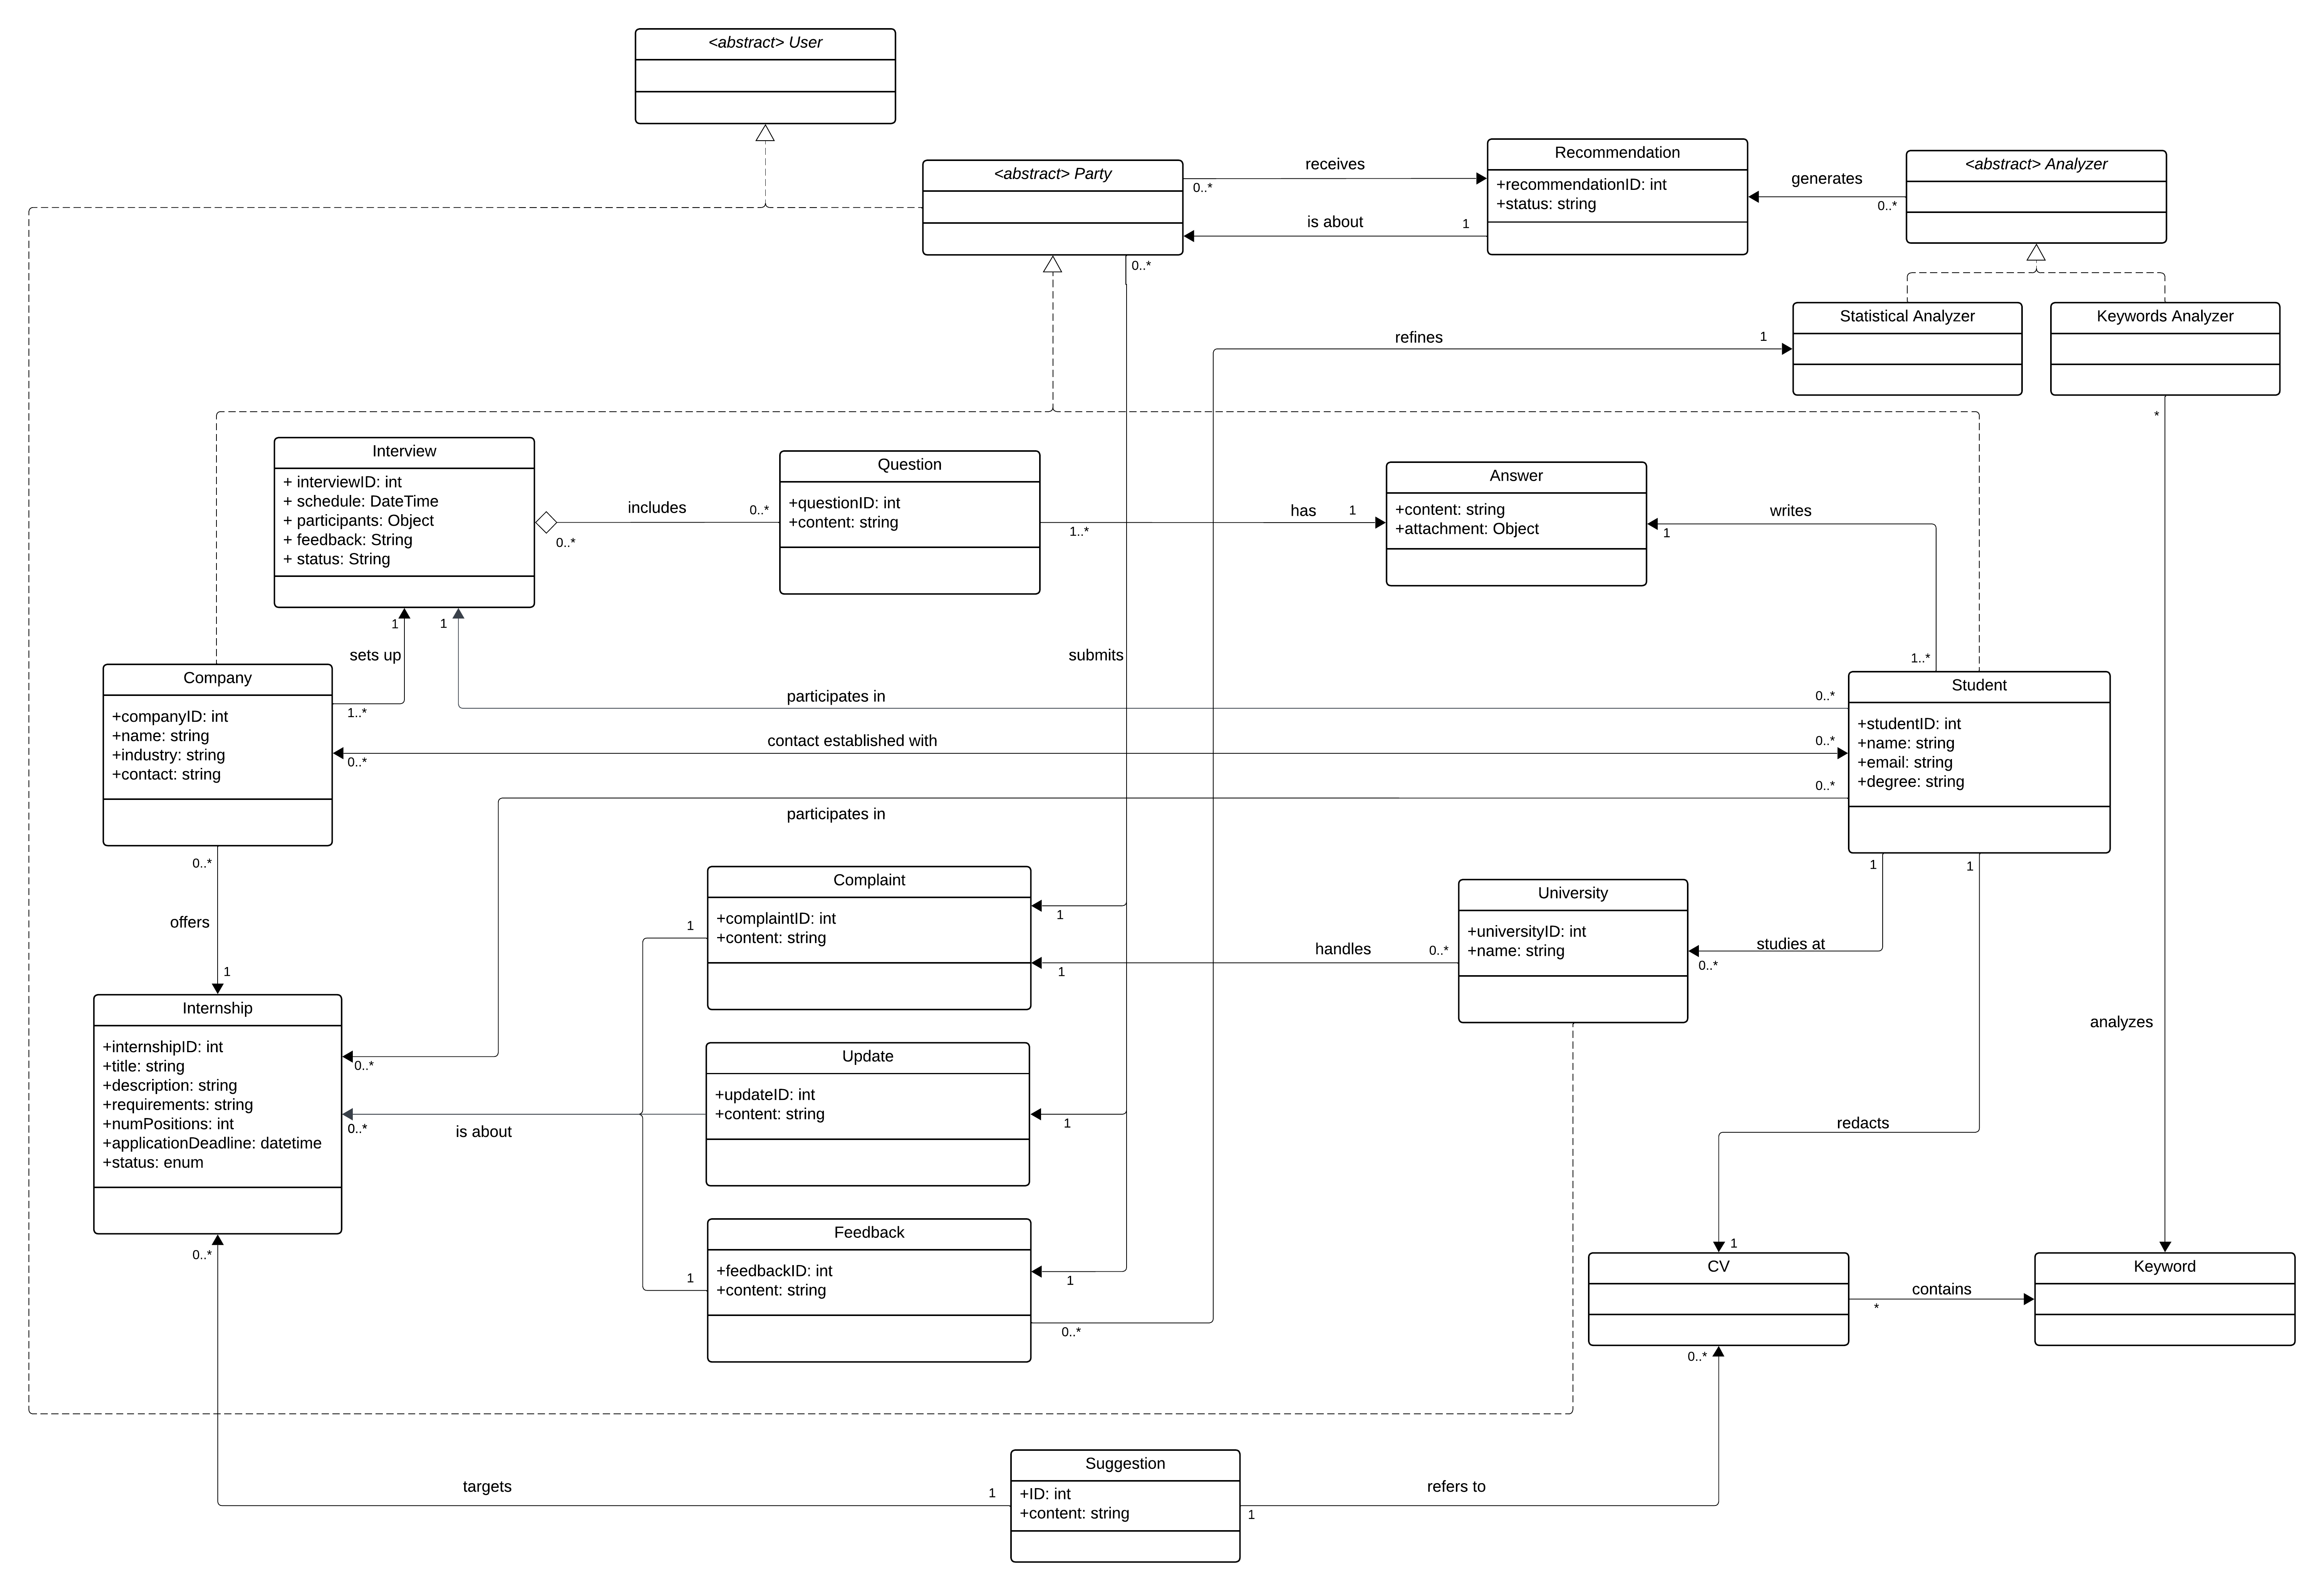
\includegraphics[width=0.9\linewidth]{LaTeXCode/images/Class Diagram - RASD.png}
        \caption{Domain-Level Class Diagram.}
        \label{fig:domain_level_class_diagrams}
    \end{center}
\end{figure}

The entities interacting with the system are modeled through a hierarchical structure to aggregate common functionalities. At the top level, the User class generalizes all the users of the system. From it, the University and Party classes derive, with the latter further specialized into the Student and Company entities.

The core of the system revolves around the concept of connecting students with internship opportunities: this is reflected in the relationships between the Student, Company, and Internship entities. The Student entity encapsulates candidate data such as personal details and educational background, which combined with the CV class, are essential to matching students with adequate internship opportunities. Companies can publish detailed internship offers that students can eventually search and apply for.

The Recommendation entity serves as a link between CVs and Internships, enabling the system to suggest the most relevant opportunities to students and identify suitable candidates for companies. This process is asymmetric, as recommendations can originate from either party since there's no full intersection in the sets of provided information in CVs and internship offers. For instance, a company might specify a requirement for expertise in a particular software or framework, which may not be explicitly detailed in a student's CV. Despite such mismatches, the system is designed to ensure potential matches are not overlooked. Any missing or unclear details can subsequently be addressed during interviews, which is the proper phase to address further clarification.

The system can generate multiple recommendations for various students for a single internship, and vice-versa, a single CV may be suitable for different internship offers. The recommendation process is powered by specialized Analyzers, which enhance accuracy through techniques such as keyword matching and statistical analysis.

Furthermore, a student remains eligible for new recommendations even while actively enrolled in an internship, since he could be interested in setting up further internships later in time.

When a recommendation is accepted, the system facilitates the next step based on the origin of the recommendation. If the recommendation has originally been sent to a company, the student receives a dual recommendation, inviting him to apply for the given internship, if interested.
 Otherwise, if the recommendation has been generated for the student, the company receives an application for their internship, similarly to applications spontaneously sent by students after searching.
 When an internship application deadline is met and both parties have accepted a recommendation, a contact is established and the internship transitions into the interview phase.

The interview process is modeled through the Interview class, which provides a structured framework for evaluating candidates. Each Interview, which is a different entity for every candidate student, is an aggregation of multiple Questions, which are designed to be reusable across different interviews. This approach promotes modularity, allowing companies to build evaluation processes reusable in multiple interviews. The Answer class captures the responses provided by candidates during the interviews. Interviews can be performed in-platform or in-person and, eventually, details are reported in the system.

A key feature of the platform is the facilitation of feedback and communication. 
During an ongoing internship, Parties can write Messages, visible only to them, to facilitate communication and share relevant information.
At the conclusion of an internship, the Feedback class allows students and companies to provide insights about their experiences, which the system can use to refine future recommendations through the statistical analyzer. 
The Complaint class offers a mechanism for reporting and addressing issues that may arise during internships. This process is monitored by the University entity, which is the only user able to read them other than the issuer, ensuring that internships comply with established agreements and resolving disputes when necessary.

\subsection{State Diagrams}
\label{subsec:state_diagrams}

\begin{figure}[H]
    \begin{center}
        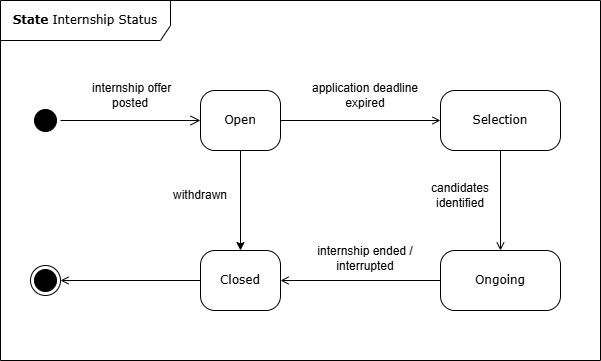
\includegraphics[width=1\linewidth]{LaTeXCode/images/State_diagram_internship.png}
        \caption{Internship Status State Diagram.}
        \label{fig:internship_state_diagram}%
    \end{center}
\end{figure}

This state diagram illustrates the lifecycle of an internship offer on the platform. It begins when an offer is posted, transitioning into the Open state, where the internship is available for applications. The offer remains open until either the application deadline expires, leading to the Selection phase, or the company withdraws it, moving directly to Closed. In the Selection state, candidates are evaluated, and if suitable candidates are identified, the process progresses to the Ongoing state, where the internship is actively taking place. Finally, upon completion or interruption of the internship, the offer transitions to the Closed state and it remains stored in the system.

\section{Product Functions}
\label{sec:product_functions}

The S\&C platform is designed to streamline the matching, selection and execution of internships, by providing functionalities that support every stage of the process. Key features include internship publication and search, automated recommendations, and monitoring tools. By integrating communication functionalities and feedback mechanisms, the platform ensures an effective experience for all users.

\begin{itemize}

    \item \textbf{Sign Up and Profile Creation} \\
    Users, identified as Students, Companies, and Universities, must sign up to the platform in order to access its functionalities. During the registration process, they create profiles by providing required personal and professional details. For students, details include additional information such as experiences, skills, and attitudes, enabling the platform to generate accurate recommendations.
    For companies, it also includes the fields in which they operate and eventually their branding elements.

    \item \textbf{Internship Publication} \\
    The platform enables companies to publish detailed and descriptive internship opportunities.
    Relevant information includes the application domain of the project along with the tasks that the student will be required to perform with the adopted technologies, if applicable.
    Furthermore, the details include the terms offered by companies: paid internship, training period or other benefits.
    These details are essential for allowing students to make informed decisions and to improve the recommendation algorithm. Companies are allowed to withdrawn internship offers before the application deadline expires.

    \item \textbf{Internship Search} \\
    Students can search for internship opportunities using filtering options based on standardized information required by the platform while posting an internship offer. This functionality ensures a user-friendly browsing experience, allowing students to efficiently find internships aligned with their preferences.

    \item \textbf{Generation of Recommendations} \\
    The platform automatically generates recommendations for students based on their profiles and, asymmetrically, suggests suitable candidates to companies. 
    The system employs various strategies to provide accurate and relevant suggestions.
    Both parties can evaluate the received recommendations and decide to accept or decline them based on their interests.

    \item \textbf{Support in the Selection Process} \\
    The platform facilitates the selection process by enabling companies to contact the candidates, schedule interviews and collect responses from students to questions shared by the company for their evaluation. In the end, it reports to students the outcomes of their interviews.

    \item \textbf{Communication Functionalities and Monitoring} \\
    The platform supports communication between students and companies, allowing them to provide updates about the status and progress of their ongoing internships and monitor them. 
    Communication of problems and complaints is made possible through private spaces.
    Universities can monitor internships to handle complaints and issue them when possible, interrupting internships if necessary.

    \item \textbf{Collecting Feedback} \\
    To improve its recommendation system, the platform gathers feedback from students and companies both during and after internships. This feedback loop allows a continuous refinement, to better address the interests of parties over time.

    \item \textbf{Personalized Suggestions} \\
    The platform assists users by providing personalized suggestions to produce more appealing descriptions. In particular, it provides suggestions to students for improving their profiles and
    it offers guidance to companies on how to optimize their internship descriptions.
\end{itemize}

\subsection{Requirements}
\label{subsec:requirements}

\newcounter{req}
\setcounter{req}{1}
\newcommand{\creq}{\thereq\stepcounter{req}}

In this section, the requirements for the system to be developed are outlined:

%Format: [condition][subject][action][object][constraint of action]
        
        \textbf{[R\creq]} Upon request, the system shall allow the User to sign up to the platform, as long as they submit all the required information, they don't already have a profile in the platform and their identity and role (Student, Company or University) are verified.

        \textbf{[R\creq]} Upon request, the system shall allow the requesting User to log in to the platform, granting him access to their profile as long as their authentication is successful.

        \textbf{[R\creq]} Upon request, the system shall allow the requesting User to update their profile, as long as they provide all the necessary information.

        \textbf{[R\creq]} Upon request, the system shall allow a Company to publish a new internship offer, as long as it provides all the required information and the latter is compliant with platform guidelines.

        \textbf{[R\creq]} Whenever a Company publishes an internship offer, the system shall add it to the list of all the internship offers.

        \textbf{[R\creq]} Upon request, the system shall allow the requesting Company to update information for any of their open internship offers, as long as it provides all the necessary information.

        \textbf{[R\creq]} Upon request, the system shall allow the requesting Company to withdraw any of their open internship offers.
        
        \textbf{[R\creq]} Upon request, the system shall allow a Student to search for desired internship offers by applying optional filters to the list.

        \textbf{[R\creq]} Whenever receiving a list of filter attributes for searching internship offers, the system shall return the list of all the offers matching the selected criteria.

        \textbf{[R\creq]} Upon request, the system shall allow the requesting Student to apply to an internship offer, as long as that offer's application deadline has not expired.

        \textbf{[R\creq]} Whenever a Student applies for an internship offer, the system shall add them to the list of candidates for that offer.

        \textbf{[R\creq]} Whenever a Student applies for an internship offer, the system shall mark all the "Unhandled" recommendations of that Student about that internship offer as "Accepted".

        \textbf{[R\creq]} Whenever a Student applies for an internship offer, the system shall discard all the "Unhandled" recommendations of the Company offering it about that Student in the context of that offer.

        \textbf{[R\creq]} Whenever an internship offer is withdrawn by its publishing Company, the system shall discard all applications to that offer.

        \textbf{[R\creq]} Whenever an internship offer is withdrawn by its publishing Company, the system shall discard all generated recommendations linked to that offer.

        \textbf{[R\creq]} Whenever a recommendation aimed at a Party is generated, the system shall add that recommendation to that Party's profile, as long as there is not another "Unhandled" recommendation about the other Party in the context of the same offer.

        \textbf{[R\creq]} Whenever a new Student signs up to the platform, the system shall generate, for every internship offer matching that Student's data, a recommendation about them aimed at the Company advertising that offer, as long as the latter's application deadline has not expired.

        \textbf{[R\creq]} Whenever a Student updates their profile, the system shall generate, for every internship offer matching that Student's updated data, a recommendation about them aimed at the Company advertising that offer, as long as the latter's application deadline has not expired.

        \textbf{[R\creq]} Whenever a Company publishes a new internship offer, the system shall generate, for every Student matching with that internship offer's data, a recommendation about it aimed at that Student.

        \textbf{[R\creq]} Whenever a Company updates data for an internship offer, the system shall generate, for every Student matching with that internship offer's updated data, a recommendation about it aimed at that Student.

        \textbf{[R\creq]} Whenever an internship offer is withdrawn by its publishing Company or its application deadline expires, the system shall discard all the recommendations about it, regardless of whether they have been accepted or not.

        \textbf{[R\creq]} Upon request, the system shall allow the requesting Party to manage their received recommendations by accepting or refusing them, if those have not already expired.

        \textbf{[R\creq]} Whenever a Student accepts one of their received recommendations, the system shall apply the requesting Student to the internship offer to which the recommendation refers.

        \textbf{[R\creq]} Whenever a Company accepts one of their received recommendations, the system shall generate a symmetric recommendation to the corresponding Student and add it to the latter's list of recommendations, as long as the generated recommendation is not already present in it.

        \textbf{[R\creq]} After the application deadline of an internship has expired, the system shall allow the publishing Company to contact a Student who had previously applied to that offer in order to plan a future interview with them, if none has been planned yet.

        \textbf{[R\creq]} Whenever a Student receives an interview proposal, the system shall allow that Student to either accept it or refuse it by providing a reason.

        \textbf{[R\creq]} Whenever an interview has to be carried out in-platform, the system shall allow the interviewing Company to submit questions to the Student involved.

        \textbf{[R\creq]} Whenever a Company submits questions to a Student for an in-platform interview, the system shall allow that Student to answer those questions, reporting them to the interviewing Company.

        \textbf{[R\creq]} Upon request, the system shall allow a Company to evaluate the answers received from a Student in one of their interviews, by registering that interview's result.

        \textbf{[R\creq]} Whenever a Company evaluates an interview (both in-platform and in-person), the system shall inform the corresponding Student of the registered outcome.  

        \textbf{[R\creq]} Whenever the interview results for all the candidates for an internship offer have been registered into the platform, the system shall close the selection process of that offer. 

        \textbf{[R\creq]} Upon request, the system shall allow the requesting Party to provide new information about any of the ongoing internships in which that Party is involved.

        \textbf{[R\creq]} Upon request, the system shall yield to the requesting Party all the information about one of the ongoing internships it is involved in.

        \textbf{[R\creq]} Upon request, the system shall allow the requesting Party to report a problem occurring in one of the ongoing internships it is involved in.

        \textbf{[R\creq]} When receiving a problem report about an internship from a Party, the system shall forward it to the University of the Student involved in that internship.

        \textbf{[R\creq]} Upon request, the system shall allow the requesting University to handle a received problem regarding an ongoing internship in which one of its Students is taking part.

        \textbf{[R\creq]} Upon request, the system shall allow the requesting Party to report feedback about an internship in which it has been actively involved, if that internship has been completed.

        \textbf{[R\creq]} Whenever receiving feedback about a completed internship, the system shall process it in order to improve the process for generating recommendations for the future.

        \textbf{[R\creq]} Upon request, the system shall provide a Student with targeted suggestions for optimizing its profile, enabling the Student to improve its appeal and relevance for obtaining more internship offers in the future, if such optimizations can be found.

        \textbf{[R\creq]} Upon request, the system shall provide a Company with targeted suggestions for optimizing a selected internship offer, enabling the Company to make it more attractive to Students and to improve its visibility for the future, if such optimizations can be found.
        
\section{User Characteristics}
\label{sec:User_characteristics}%

The S\&C platform is designed for three categories of users:

\begin{itemize}
    \item [\textbf{Students}] University students seeking internships. They are typically proficient users, familiar with app navigation and common interaction patterns such as registration, profile management, and document uploads (e.g., CVs). Their primary motivation is to find internships aligned with their skills and career goals efficiently. Students generally access the platform a few times each week while searching for internships and reviewing recommendations, with increased frequency during the interview phases.
    
    \item [\textbf{Companies}] Human Resources professionals responsible for posting internship opportunities, reviewing candidate recommendations, conducting the selection process, and providing feedback on ongoing internships. These users may vary in technical proficiency with the platform, but expect a straightforward interface to accomplish core tasks efficiently.
    They typically interact with the platform multiple times daily during work hours, particularly during active recruitment periods.
    
    \item [\textbf{Universities}] University staff responsible for monitoring internship outcomes and addressing their student-related complaints during internships. While their technical expertise may vary, they require tools for monitoring and complaint management. They have minimal involvement in day-to-day activities on the platform. The typical number of interactions can be a few times per week, depending on the number of students they manage.
\end{itemize}

All users expect a user-friendly interface and support features. The system accommodates varying levels of technical proficiency and ensures accessibility for all user groups.

\section{Assumptions, Dependencies and Constraints}
\label{sec:assumptions_dependencies_constraints}%

\subsection{Domain Assumptions}
\label{subsec:domain_assumptions}%

\newcounter{da}
\setcounter{da}{1}
\newcommand{\cda}{\theda\stepcounter{da}}

    \textbf{[DA\cda]} Users always interact with the system only through a device with a reliable connection to the Internet.

    \textbf{[DA\cda]} People who sign up to the platform have an active email address that they can provide to the system.

    \textbf{[DA\cda]} People who sign up to the platform can access the mailbox of the email address provided during the registration process.

    \textbf{[DA\cda]} People who are not Students, Companies or Universities never disguise themselves as being one of those.

    \textbf{[DA\cda]} Students signing up to the platform belong to one of the Universities which have already registered on the platform.

    \textbf{[DA\cda]} Users never provide false information about themselves.

    \textbf{[DA\cda]} Companies never provide false information about their internship offers.

    \textbf{[DA\cda]} Students never withdraw any of their applications to internship offers (equivalently, they apply for internships only if those match their interests and if they really want to undertake them).

    \textbf{[DA\cda]} For each of their internship offers, Companies always try to set up interviews with all and only the Students who have submitted an application.

    \textbf{[DA\cda]} Companies always finalize the selection process and bring it to completion, even if they haven't found any fitting candidate among the interviewed students.

    \textbf{[DA\cda]} Complaints inserted into the system always refer to events that have happened during the internship they are related to.

    \textbf{[DA\cda]} Users regularly upload information about the ongoing internships

    \textbf{[DA\cda]} Universities always act on received complaints and solve exposed issues, promptly terminating the internship if necessary.

    \textbf{[DA\cda]} Feedback inserted into the system after performing an internship is always meaningful to be fed to the statistical analysis.    

\begin{center}
\end{center}


    \chapter{Specific Requirements}
    \label{ch:specific_requirements}%
    
\section{External Interface Requirements}
\label{sec:external_interface_requirements}

\subsection{User Interfaces}
\label{subsec:User_interfaces}

\begin{figure}[H]
    \begin{center}
        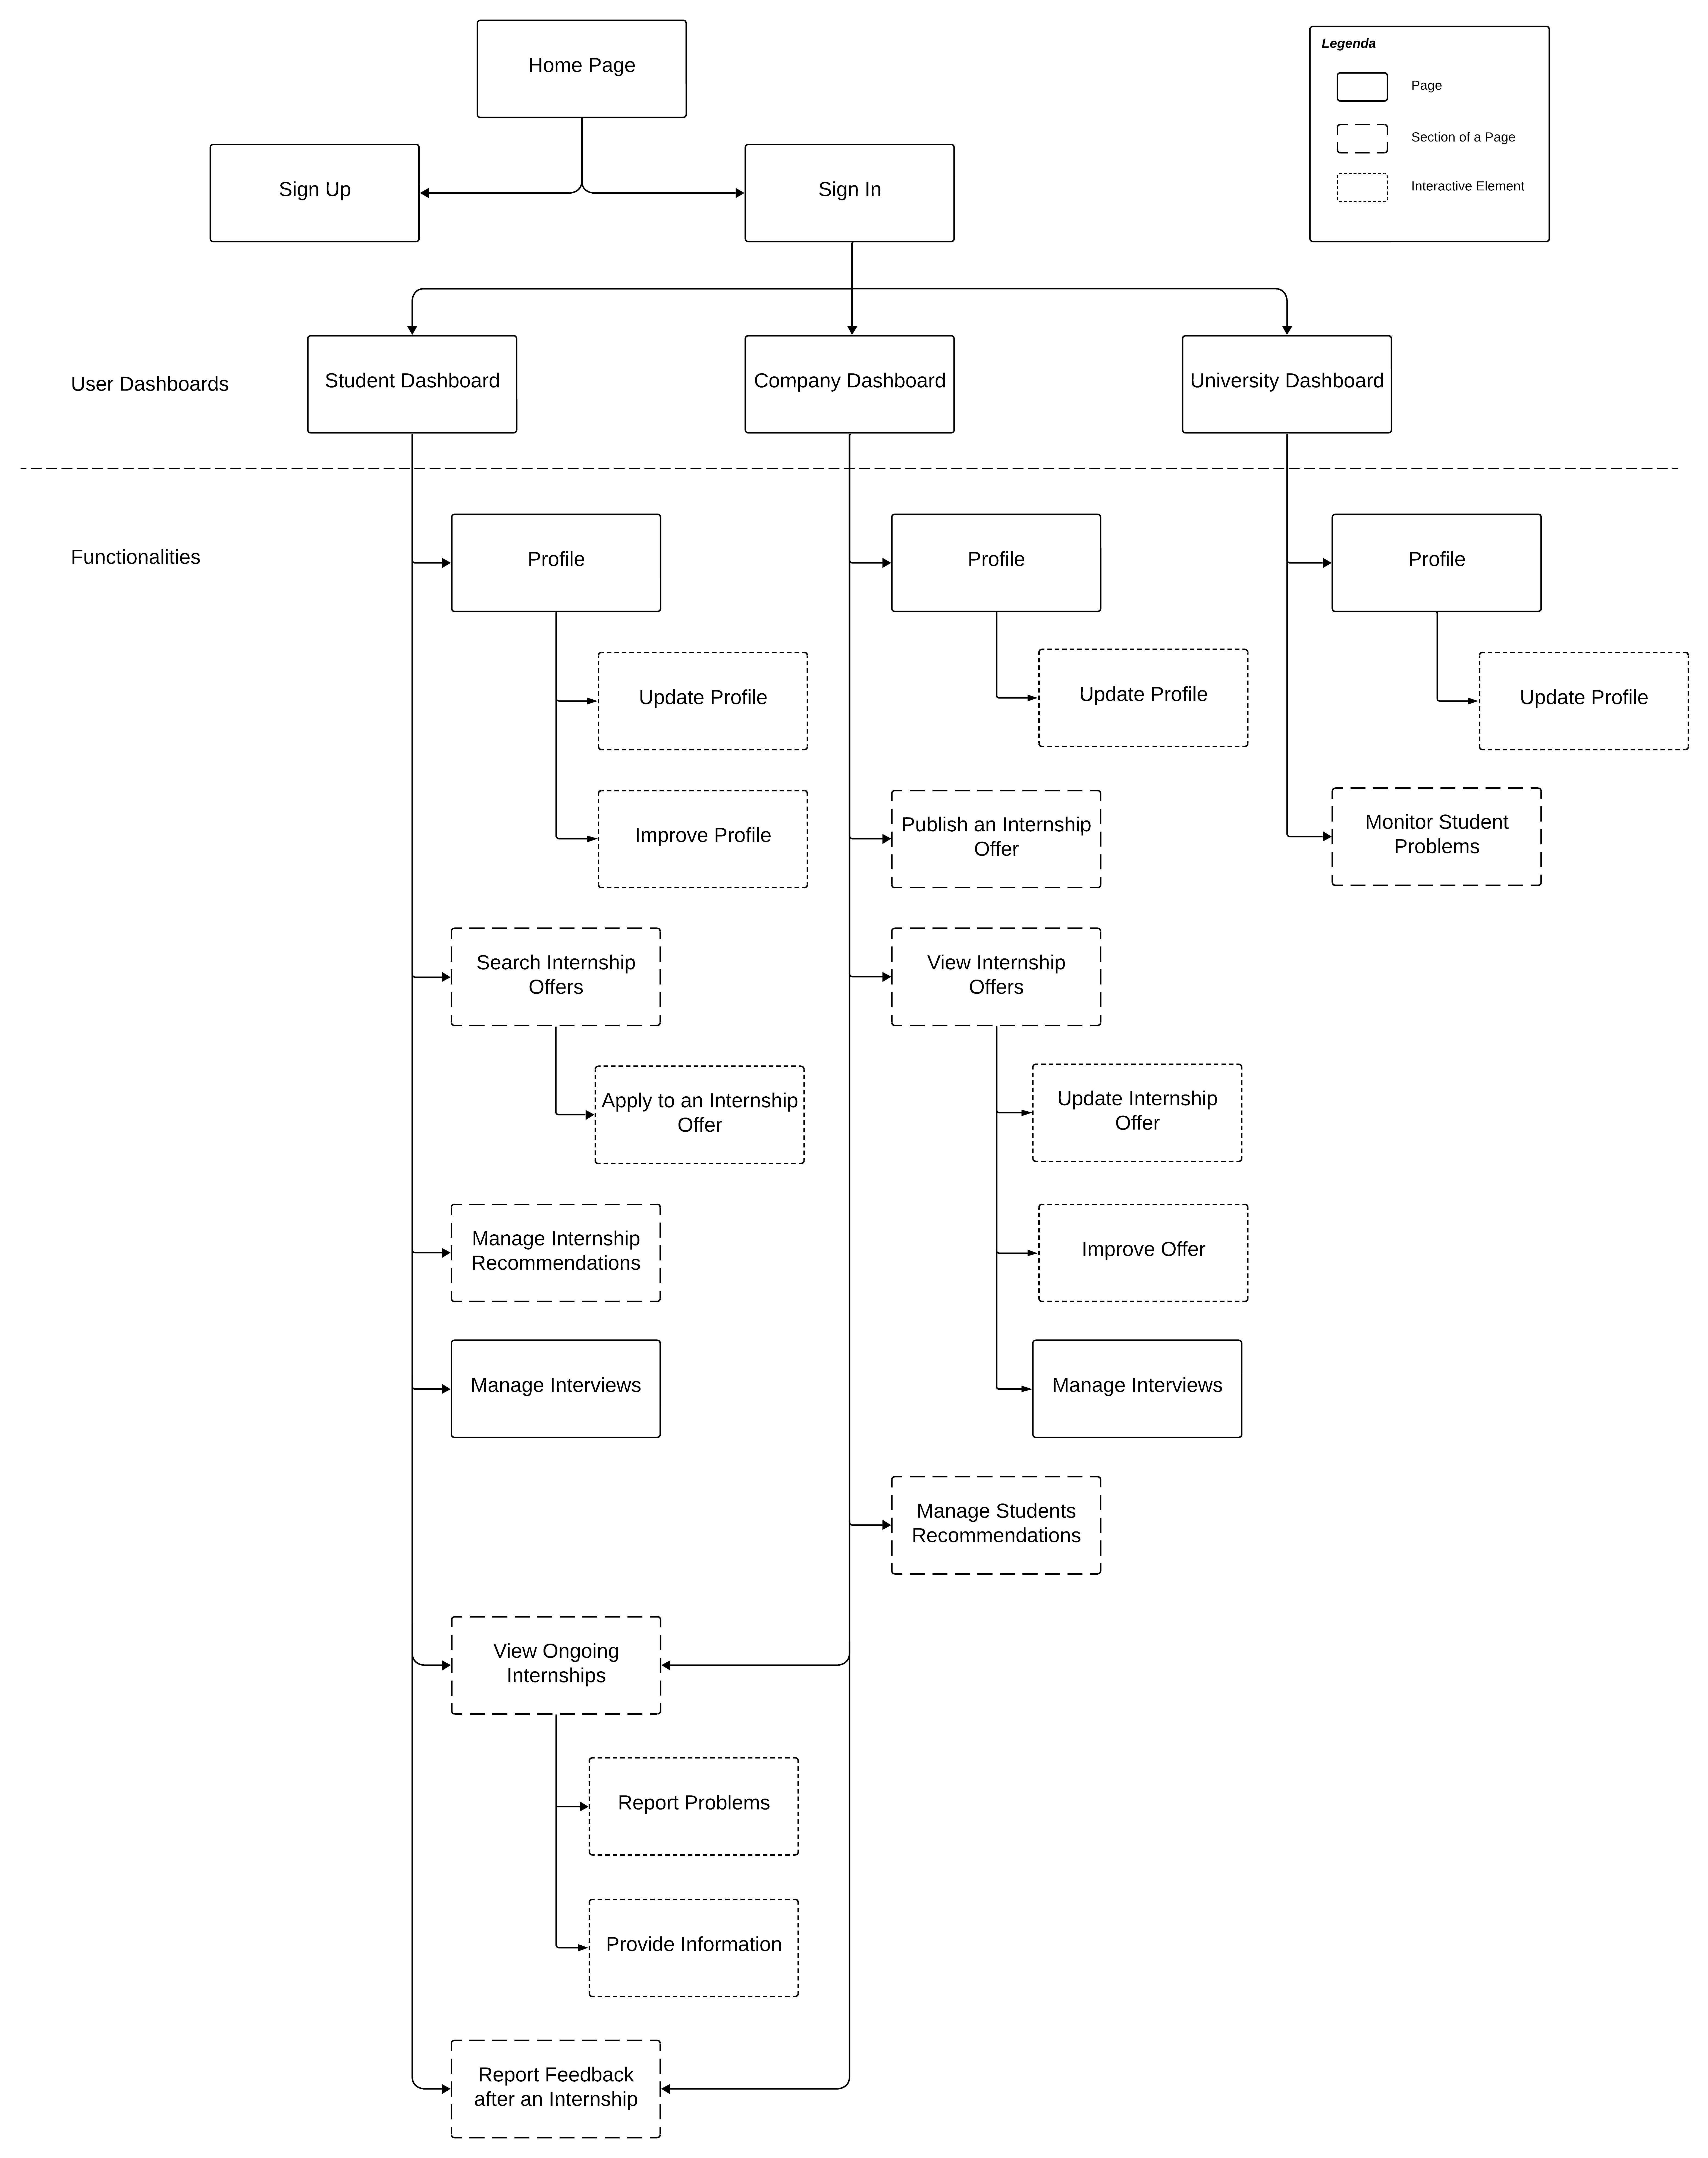
\includegraphics[width=0.7\linewidth]{LaTeXCode/images/webapp_map_workflow.png}
        \caption{WebApp Map} 
        \label{fig: webapp_map}
    \end{center}
\end{figure}

\newpage

The platform's user interface shall be designed to ensure usability and interactivity, adhering to web standards, briefly discussed in \hyperref[sec:standards_compliance]{\uline{3.4.1. Standards Compliance}}. The interface shall adapt responsively to various device displays, providing an intuitive layout and functionality across all the supported devices. Interface elements shall be organized in a layout that prioritizes clarity and ease of navigation for all the users.

Below is a description of the primary interfaces needed, as visually displayed in the above map, and how they should be grouped and structured:

\subparagraph{Home Page}
This page serves as the entry point to the platform and offers:
\begin{itemize}
    \item \textbf{Sign-Up (Register)}: A page to start the initial registration process for the three distinct user types.
    \item \textbf{Sign-In (Login)}: A page to perform login that redirects authenticated users to their respective dashboards.
\end{itemize}

\subparagraph{User Dashboards}
Each user type is provided with a personalized dashboard, divided into sections offering different functionalities:

\begin{enumerate}
    \item \textbf{Student Dashboard}
    \begin{itemize}
        \item \textbf{Search Internship Offers}: a section that includes a search bar with filtering options to search offers. Each result of the query is an interactive element displaying an overview of the information related to an internship offer; clicking on the internship offer expands its details and enables an interactive element to apply to it.
        \item \textbf{Manage Internship Recommendations}: a section listing the received internship recommendations. Each recommendation is an interactive element, and students can visualize details about the internship offer associated to each recommendation and accept, reject, or postpone the recommendations.
        \item \textbf{Manage Invitations}: a section displaying interview invitations. Each invitation is an interactive element, and Students can confirm or decline, providing a reason, based on their availability. Questions posted by companies are also made available in a parallel section as interactive elements and are displayed here.
        \item \textbf{Monitor Interviews}: a section displaying the status of interview processes. Each interview is an interactive element, and Students can visualize the status and outcome of each interview.
        \item \textbf{View Internships}: a section displaying all ongoing and past internships. Each internship is an interactive element and based on its status, it allows students to:
        \begin{itemize}
            \item \textbf{Report Problems}: an interactive element to report problems to be handled by the university.
            \item \textbf{Report Feedback after an Internship}: an interactive element to give feedback upon completion of an internship.
        \end{itemize}
        \item \textbf{Provide Information}: a section where to write relevant information during an internship and communicate with the other party.
        \item \textbf{Profile}: a page displaying all the student's information and including:
        \begin{itemize}
            \item \textbf{Update Profile}: an interactive element for updating personal and academic information.
            \item \textbf{Improve Profile}: an interactive element suggesting optimizations based on the content of the profile and CV.
        \end{itemize}
    \end{itemize}

    \item \textbf{Company Dashboard}
    \begin{itemize}      
        \item \textbf{Publish an Internship Offer}: an interactive element to publish new internship offers.
        \item \textbf{View Internship Offers}: a section listing all published internship offers. Each internship offer is an interactive element displaying an overview of the information related to an internship offer; clicking on the internship offer expands its details.
        Via interactive elements it allow the company to:
        \begin{itemize}
            \item \textbf{Update an Internship Offer}: an interactive element for updating the offer information.
            \item \textbf{Improve Offer}: an interactive element to receive optimizations based on the offer details.
            \item \textbf{Shortcut - Manage Interviews}: a shortcut allowing companies to handle interview invitations and post questions to candidates about a specific internship offer.
            \item \textbf{Shortcut - Manage Student Recommendations}: a shortcut allowing companies to manage students recommendations about a specific internship offer.
        \end{itemize}
        \item \textbf{Manage Student Recommendations}: a section listing student's recommendations. Each recommendation is an interactive element, and the company can visualize the profile of the recommended student and accept, reject, or postpone it.
        \item \textbf{Manage Invitations}: a section offering an interactive element to create and display interview invitations. Each invitation is an interactive element, and the company can monitor the status of each of them. Questions posted by companies are also made available in A parallel section allows companies to post new questions to candidates and visualize the answers provided by them to previously submitted questions.
        \item \textbf{Manage Interviews}: a section displaying the status of interview processes. Each interview is an interactive element, and companies can update their status, also finalizing the selection process, and provide a feedback when an interview is completed.
        \item \textbf{View Internships}: a section displaying all ongoing and past internships. Each internship is an interactive element and based on its status, it allows companies to:
        \begin{itemize}
            \item \textbf{Report Problems}: an interactive element to report problems to be handled by the university.
            \item \textbf{Report Feedback after an Internship}: an interactive element to give feedback upon completion of an internship.
        \end{itemize}
        \item \textbf{Provide Information}: a section where to write relevant information during an internship and communicate with the other party.
        \item \textbf{Profile}: a page displaying all the company's information and including:
        \begin{itemize}
            \item \textbf{Update Profile}: an interactive element for updating company information.
        \end{itemize}  
    \end{itemize}

    \item \textbf{University Dashboard}
    \begin{itemize}  
        \item \textbf{Monitor Student Problems}: a section displaying issues reported by students during internships. Each report is an interactive element and provides tools to review, resolve, and update statuses.
        \item \textbf{Profile}: a page displaying all university-related information and including:
        \begin{itemize}
            \item \textbf{Update Profile}: an interactive element for updating information.
        \end{itemize} 
    \end{itemize}
\end{enumerate}

\subsection{Software Interfaces}
\label{subsec:software_interfaces}

The system is meant to be a platform-independent WebApp, which does not rely on external APIs or essential third-party software to perform its core functionalities. 
However, the system shall adhere to the following requirements:

\begin{itemize}
    \item It shall function across the most widely adopted operating systems, including but not limited to Microsoft Windows, MacOSX, Linux, Android, iOS and ChromeOS.
    
    \item It shall function across the most widely used browsers, including, but not limited to, Google Chrome, Opera, Mozilla Firefox, Safari, and Microsoft Edge, without requiring additional software installation on the user’s device.

    \item It shall interact appropriately with the chosen services or network protocols for email management, in order to carry on sign-up and sign-in functionalities.
\end{itemize}

No additional software installations or configurations are required on the user's device beyond the availability of a supported web browser.

\subsection{Communication Interfaces}
\label{subsec:communication_interfaces}

The system shall support standard communication protocols for reliable interaction between the components. Specifically, the following requirements apply:

\begin{itemize}
    \item The system shall operate over standard internet connections, including wired and wireless networks (e.g. Ethernet, Wi-Fi, mobile data).

    \item The system shall support encrypted communication/secure sessions (e.g. through TLS/SSL) to protect sensitive data, including user credentials and personal information, during transmission.

    \item The system shall utilize a widely adopted web communication protocol (such as HTTPS) to ensure secure and reliable data transmission between the user's browser and the web server.

    \item The system shall not require users to install additional software to facilitate communication.

    \item The system shall minimize communication latency to provide a responsive user experience, with server response times aligning with industry standards for web applications.
\end{itemize}

\subsection{Hardware Interfaces}
\label{subsec:hardware_interfaces}

The system shall ensure compatibility with common user devices and hosting infrastructure, designed to provide performance and accessibility.

\subsubsection{User Devices}

The platform shall support access from a wide range of devices commonly used by end-users, including but not limited to: desktop and laptop computers, tablets and smartphones.

The platform shall ensure responsiveness and usability across different device types and display resolutions, requiring hardware with free space for caching that can run modern web applications efficiently.

\subsubsection{Hosting Infrastructure}

The system shall be deployed on an infrastructure capable of supporting:

\begin{itemize}
    \item Simultaneous access by multiple users with minimal latency
    \item Data processing and storage necessary for handling user interactions and background operations
\end{itemize}

The hosting environment shall be scalable to accommodate growth in usage and computational demands while maintaining reliable service availability.

\section{Functional Requirements}
\label{sec:functional_requirements}

\begin{figure}[H]
    \begin{center}
        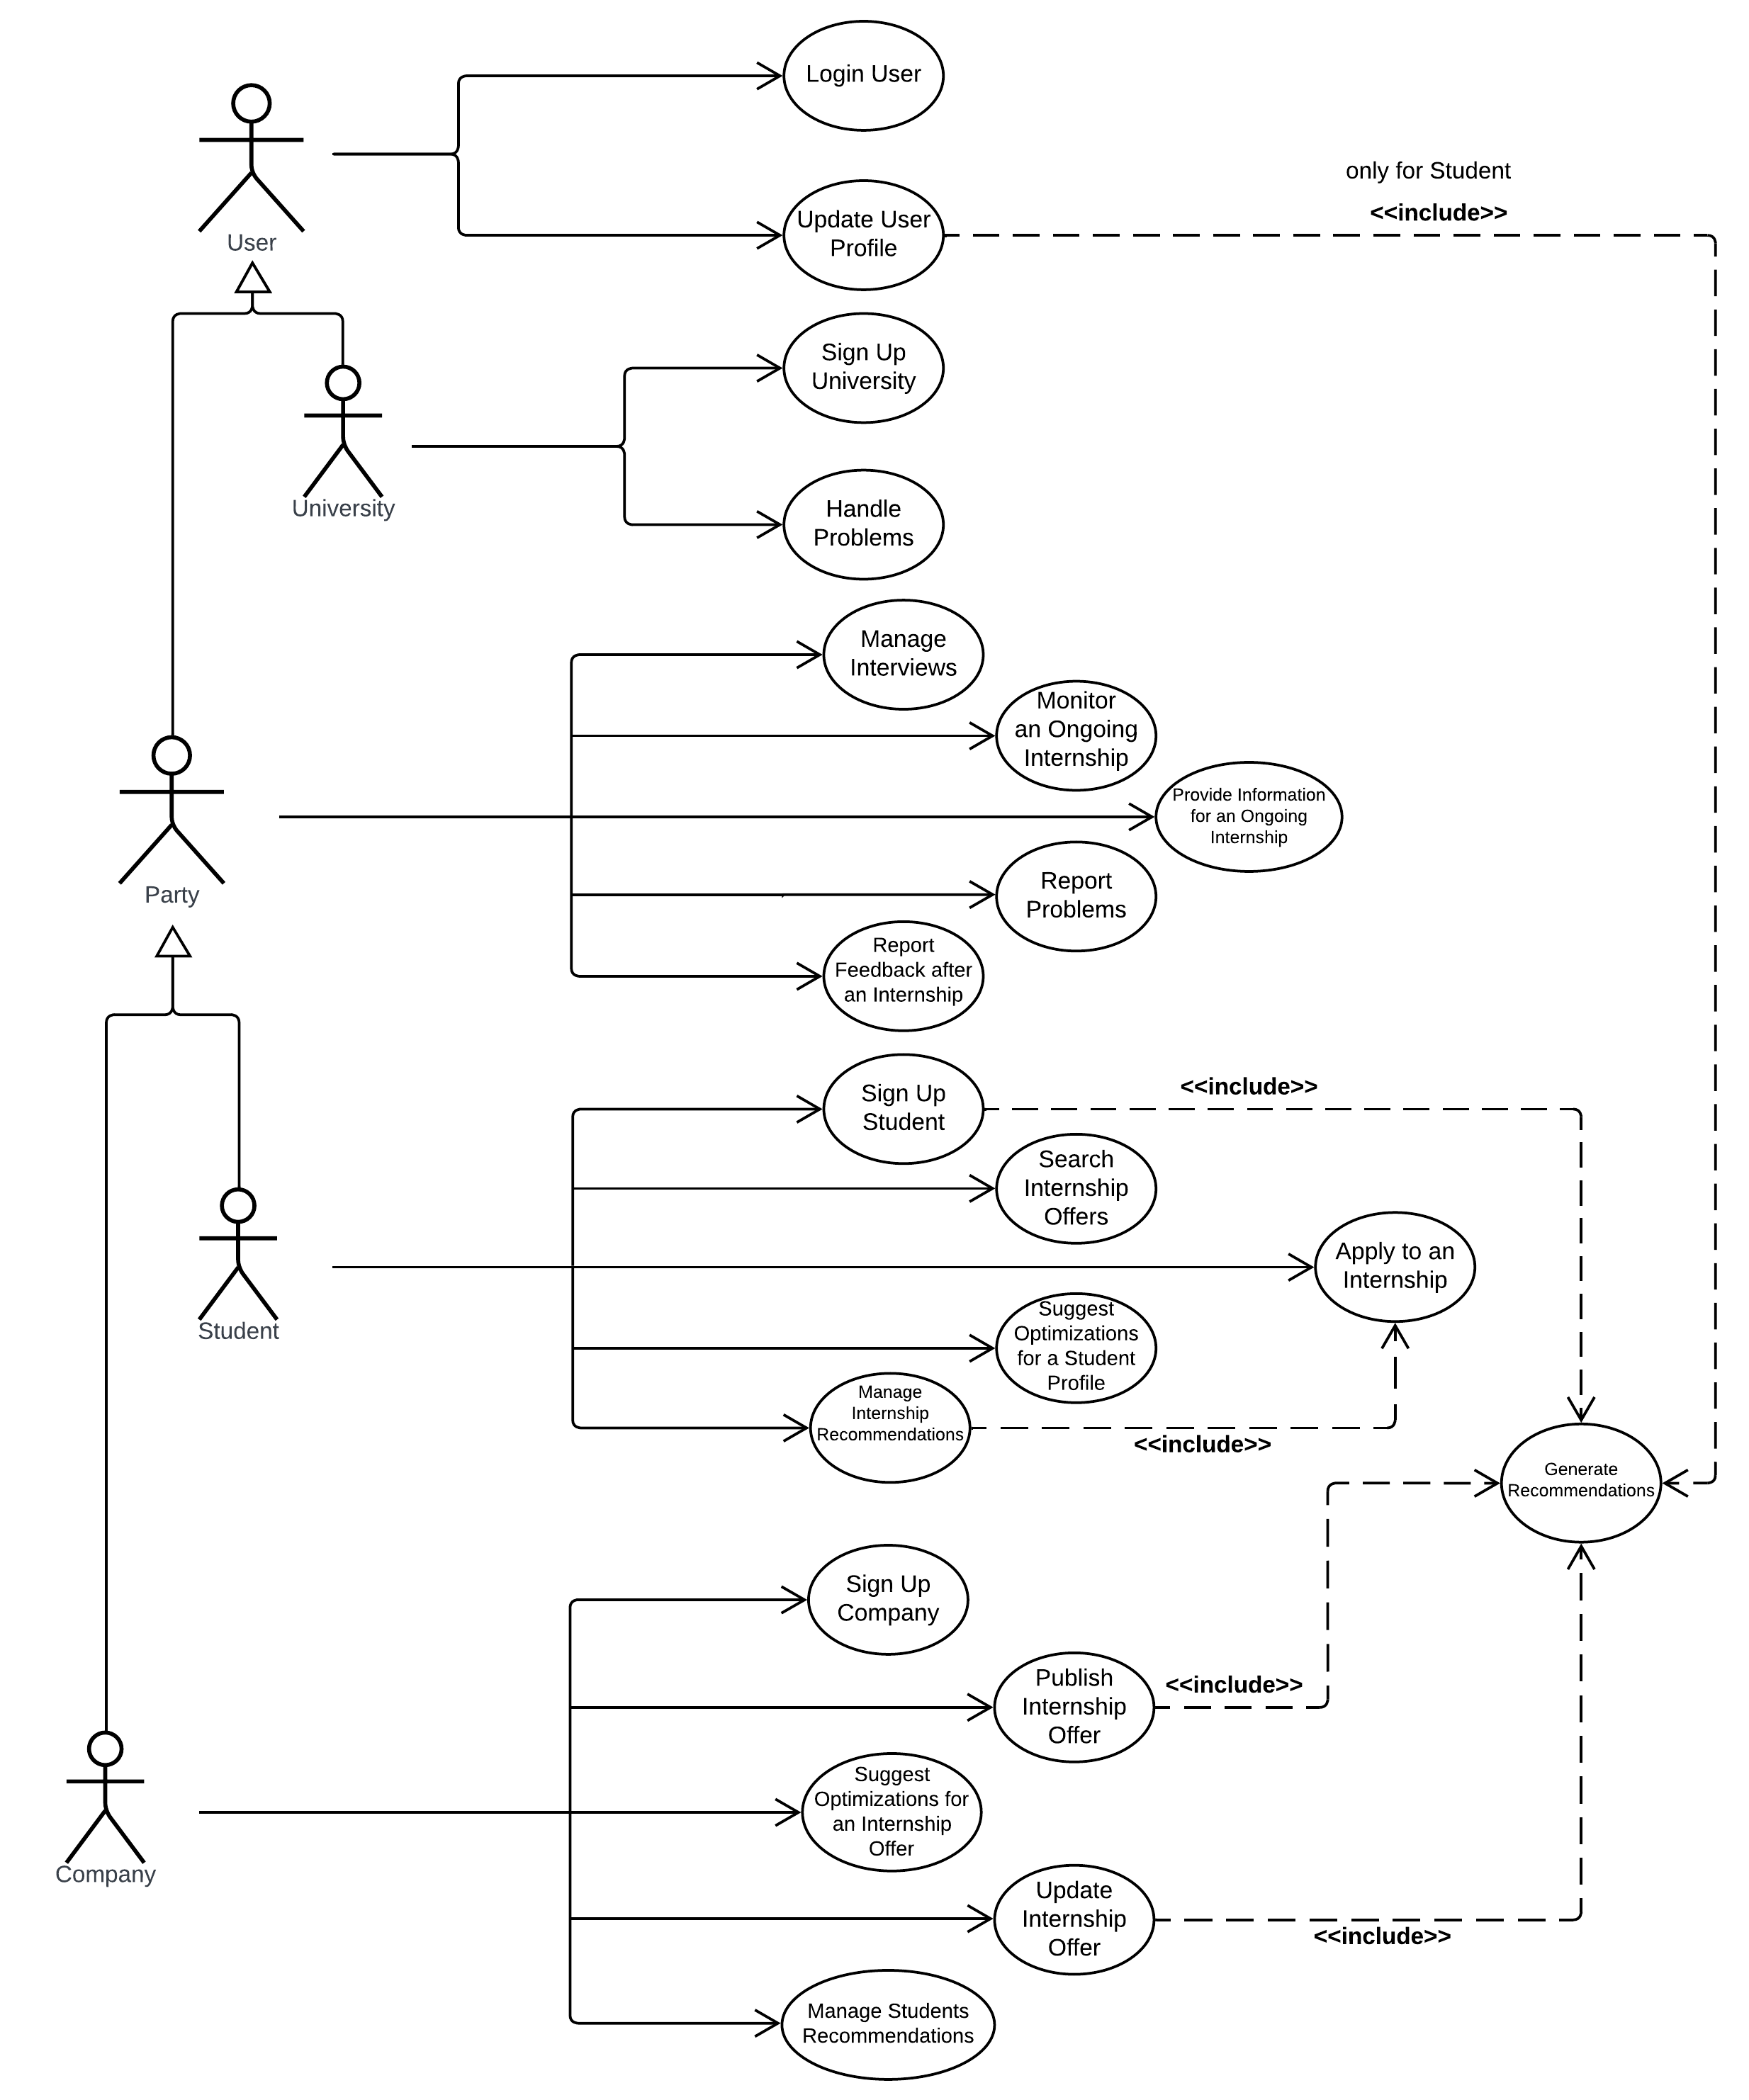
\includegraphics[width=0.9\linewidth]{LaTeXCode/images/Use Case Diagram of S&C.png}
        \caption{Use Case Diagram} 
        \label{fig:use_case_diagram}
    \end{center}
\end{figure}

\newpage
\subsection{Use Cases and Activity Diagrams}
\label{subsec: use_cases}%

\newcounter{ucsteps}
\setcounter{ucsteps}{1}
\newcommand{\cucsteps}{\theucsteps\stepcounter{ucsteps}}
\newcommand{\resetucsteps}{\setcounter{ucsteps}{1}}

\newcounter{uc}
\setcounter{uc}{1}
\newcommand{\cuc}{\theuc\stepcounter{uc}\resetucsteps}

\subsubsection*{UC\cuc . Sign Up by a Student}
\begin{center}
    \begin{longtable}{|l|p{0.75\linewidth}|}
        \hline
        \textbf{Actor}            & Student\\
        \hline
        \textbf{Entry Conditions} & The Student is not logged into the S\&C platform. \\
        \hline
        \textbf{Flow of Events}    
        & \cucsteps. On the homepage, the Student clicks the "Sign Up" button, entering the initial registration page. \\
        & \cucsteps. The Student provides the required details: User category (Student), email, password and password confirmation. \\
        & \cucsteps. The Student confirms the provided information by clicking the "Register" button. \\
        & \cucsteps. The system sends to the indicated mailbox a confirmation email with a link that expires in 24 hours for account verification purposes. \\
        & \cucsteps. The Student clicks the link in the confirmation email before it expires and logs into the platform. \\
        & \cucsteps. On the profile page, the Student completes their profile by inserting:
        name, surname, date of birth, gender, compiling its CV, selecting their university from a drop-down list and adding relevant details: skills, education, and career aspirations. \\
        & \cucsteps. The system starts an instance of the process for identifying new recommendations via the \hyperref[subsec: generate_recommendations_uc]{\uline{UC. Generate Recommendations}} functionality. \\
        \hline
        \textbf{Exit Conditions}   & The profile is complete and the Student has access to its functionalities.\\       
        \hline
        \textbf{Exceptions}       & \begin{itemize}
            \item The email address is already linked to an existing account: an error message is shown, and the Student is redirected to the login page.
            \item The password does not meet the platform's security requirements: an error message is displayed, and the Student is prompted to correct the password.
            \item Some mandatory fields are missing: the system doesn't allow the Student to complete the procedure until all the mandatory fields are filled out.
            \item The confirmation link sent to the indicated mailbox expires: all the information previously inserted into the system by the Student is discarded, and the link is invalidated.
        \end{itemize} \\
        \hline
    \end{longtable}
\end{center}

\begin{figure}[H]
    \begin{center}
         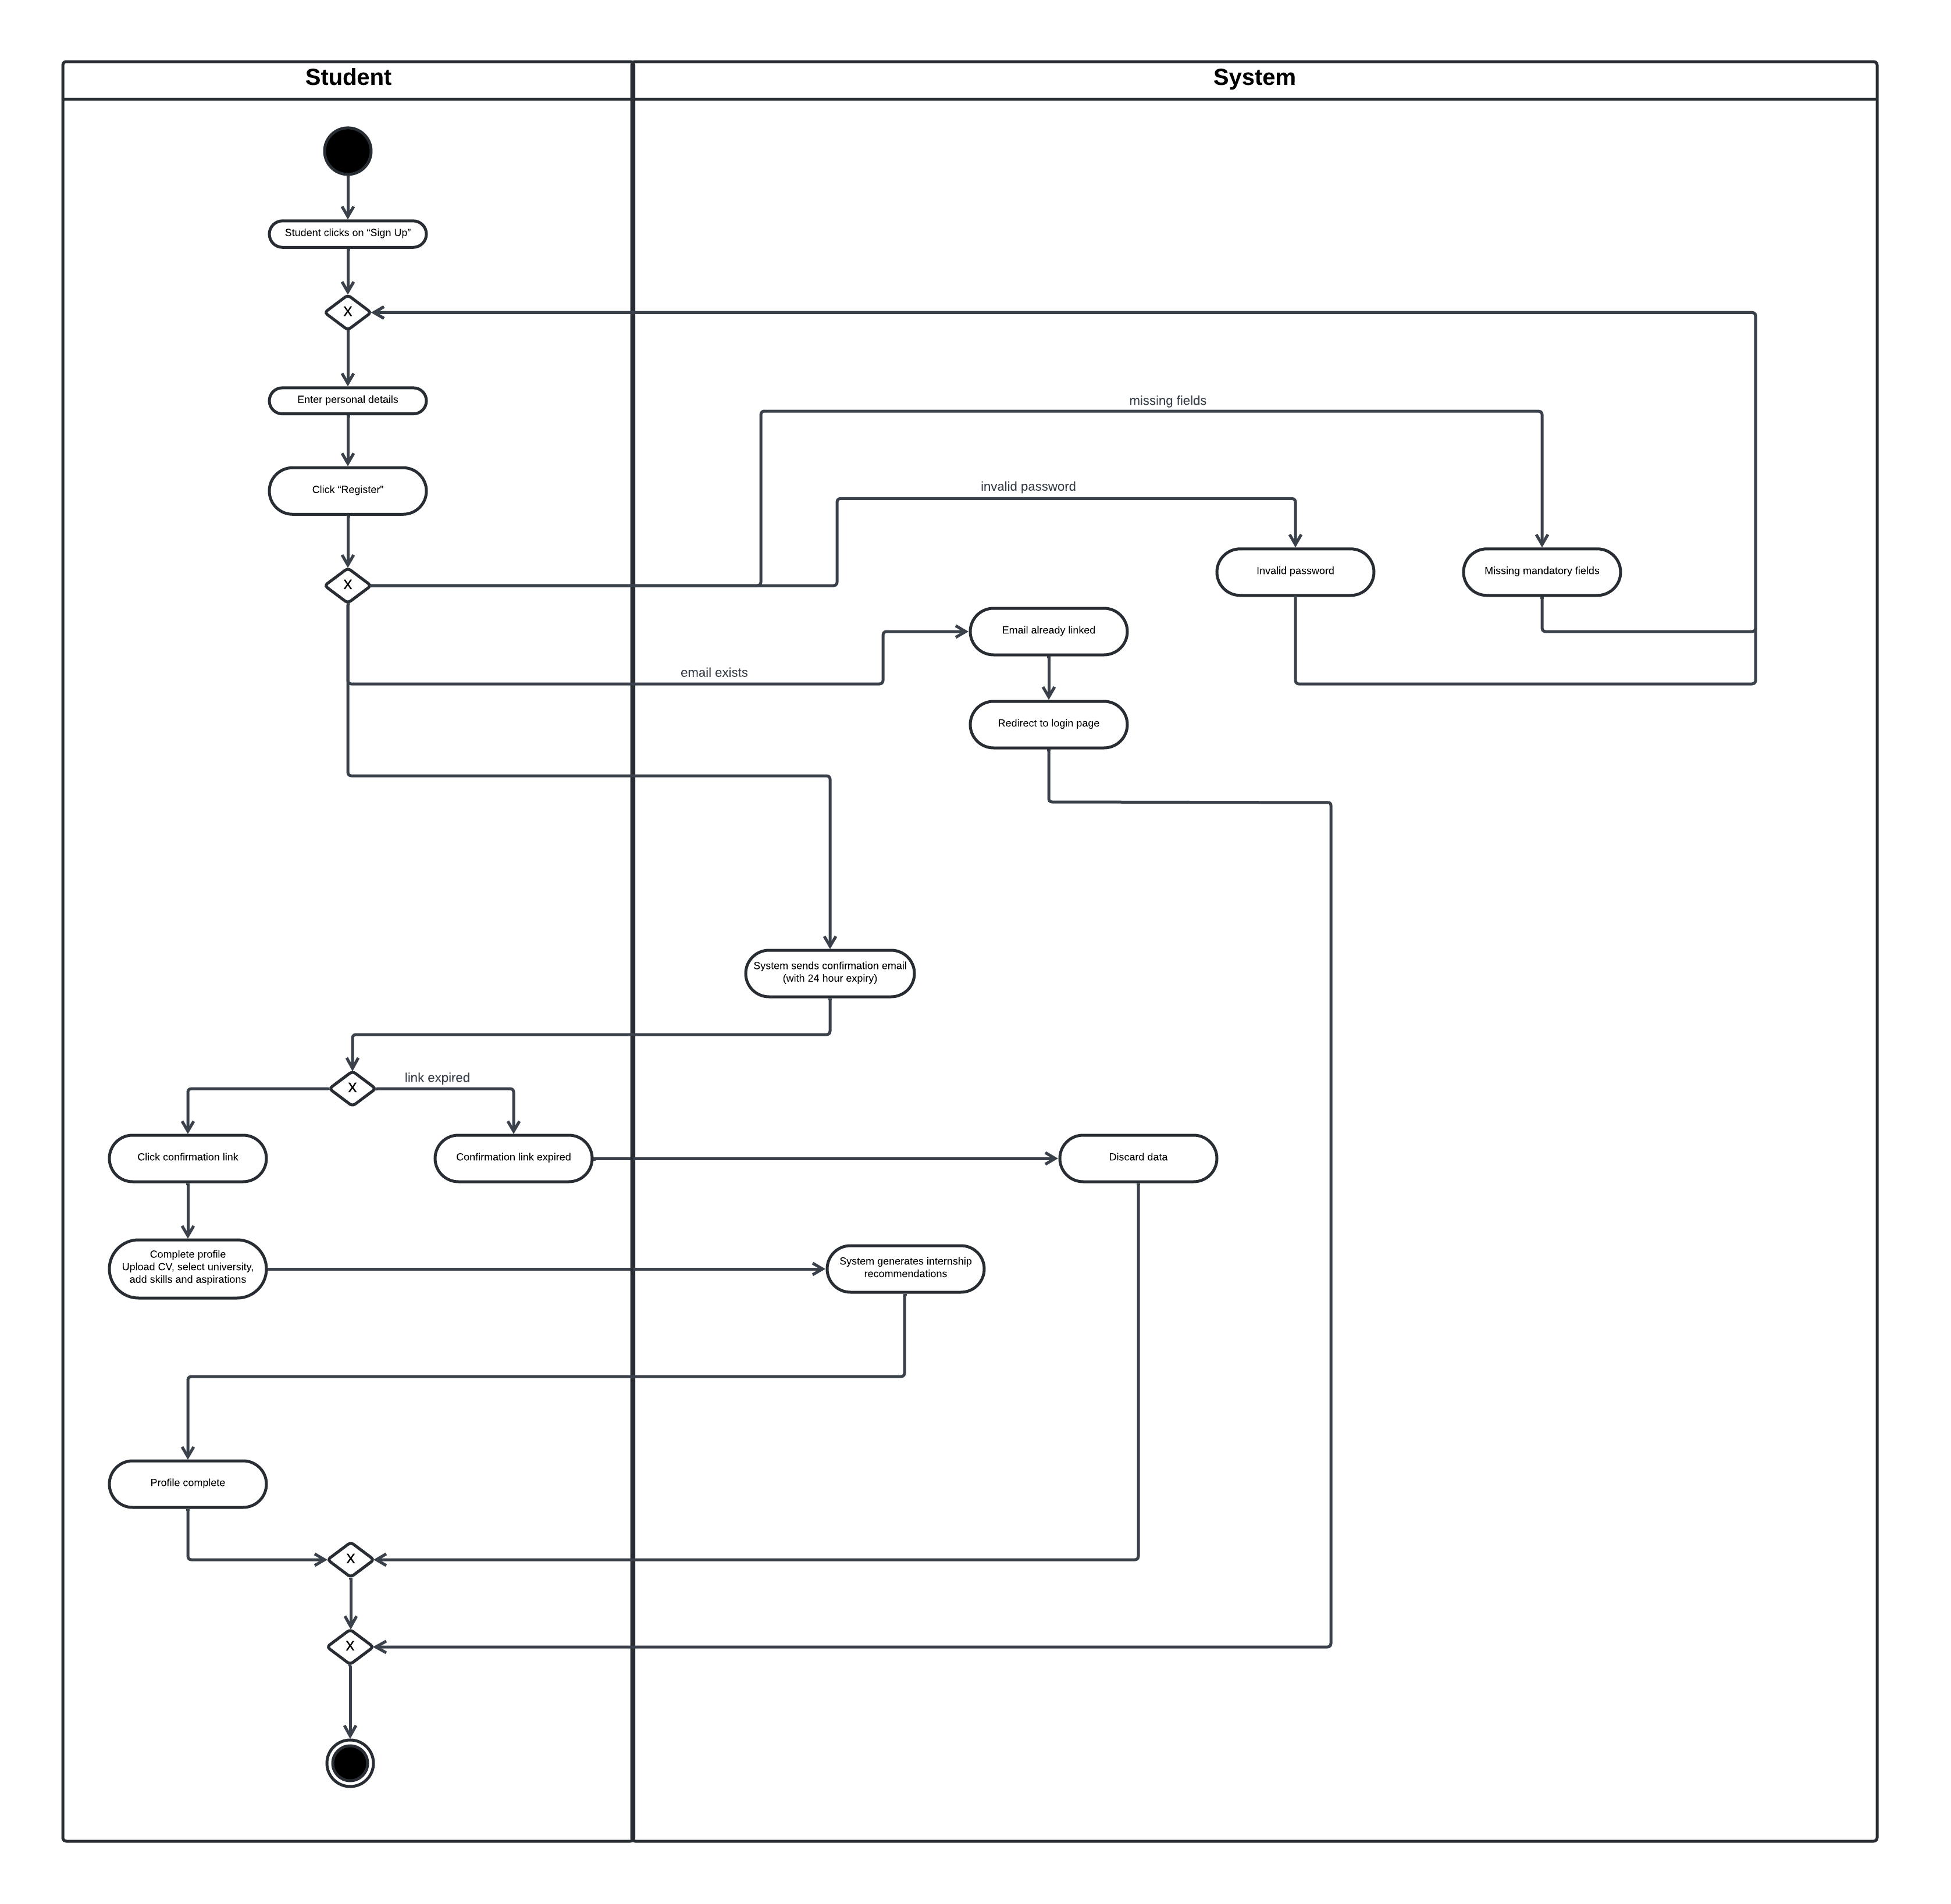
\includegraphics[width=1\linewidth]{LaTeXCode/images/activity diagram/UC1.png}
         \caption{Sign Up by a Student}
         \label{fig:signup_student_ad}
     \end{center}
\end{figure}

\newpage

\subsubsection*{UC\cuc . Sign Up by a Company}
\begin{center}
    \begin{longtable}{|l|p{0.75\linewidth}|}
        \hline
        \textbf{Actor}            & Company \\
        \hline
        \textbf{Entry Conditions} & The Company is not logged into the S\&C platform. \\
        \hline
        \textbf{Flow of Events}       
        & \cucsteps. On the homepage, the Company clicks the "Sign Up" button, entering the companies' registration page. \\
        & \cucsteps. The Company provides the required details: User category (Company), email, password and password confirmation. \\
        & \cucsteps. The Company confirms the provided information by clicking the "Register" button. \\
        & \cucsteps. The system sends to the indicated mailbox a confirmation email with a link that expires in 24 hours for account verification purposes. \\
        & \cucsteps. The Company clicks the link in the confirmation email and logs into the platform. \\
        & \cucsteps. On the profile page, the Company completes the company's profile by adding all other information and relevant details: company name, location, phone number,
        company description, mission, vision, and field in which it operates, and uploading its logo. \\
        \hline
        \textbf{Exit Conditions}   & The profile is complete and the Company has access to all its functionalities. \\       
        \hline
        \textbf{Exceptions}       & \begin{itemize}
            \item The email address is already linked to an existing account: an error message is shown, and the Company is redirected to the login page.
            \item The password does not meet the platform security requirements: An error message is displayed, and the Company is prompted to correct the password.
            \item Some mandatory fields are missing: the system does not allow the Company to complete the procedure until all the mandatory fields are filled out.
            \item The confirmation link sent to the indicated mailbox expires: all information previously inserted into the system by the Company is discarded and the link is invalidated.
        \end{itemize}\\
        \hline
    \end{longtable}
\end{center}

\begin{figure}[H]
    \begin{center}
         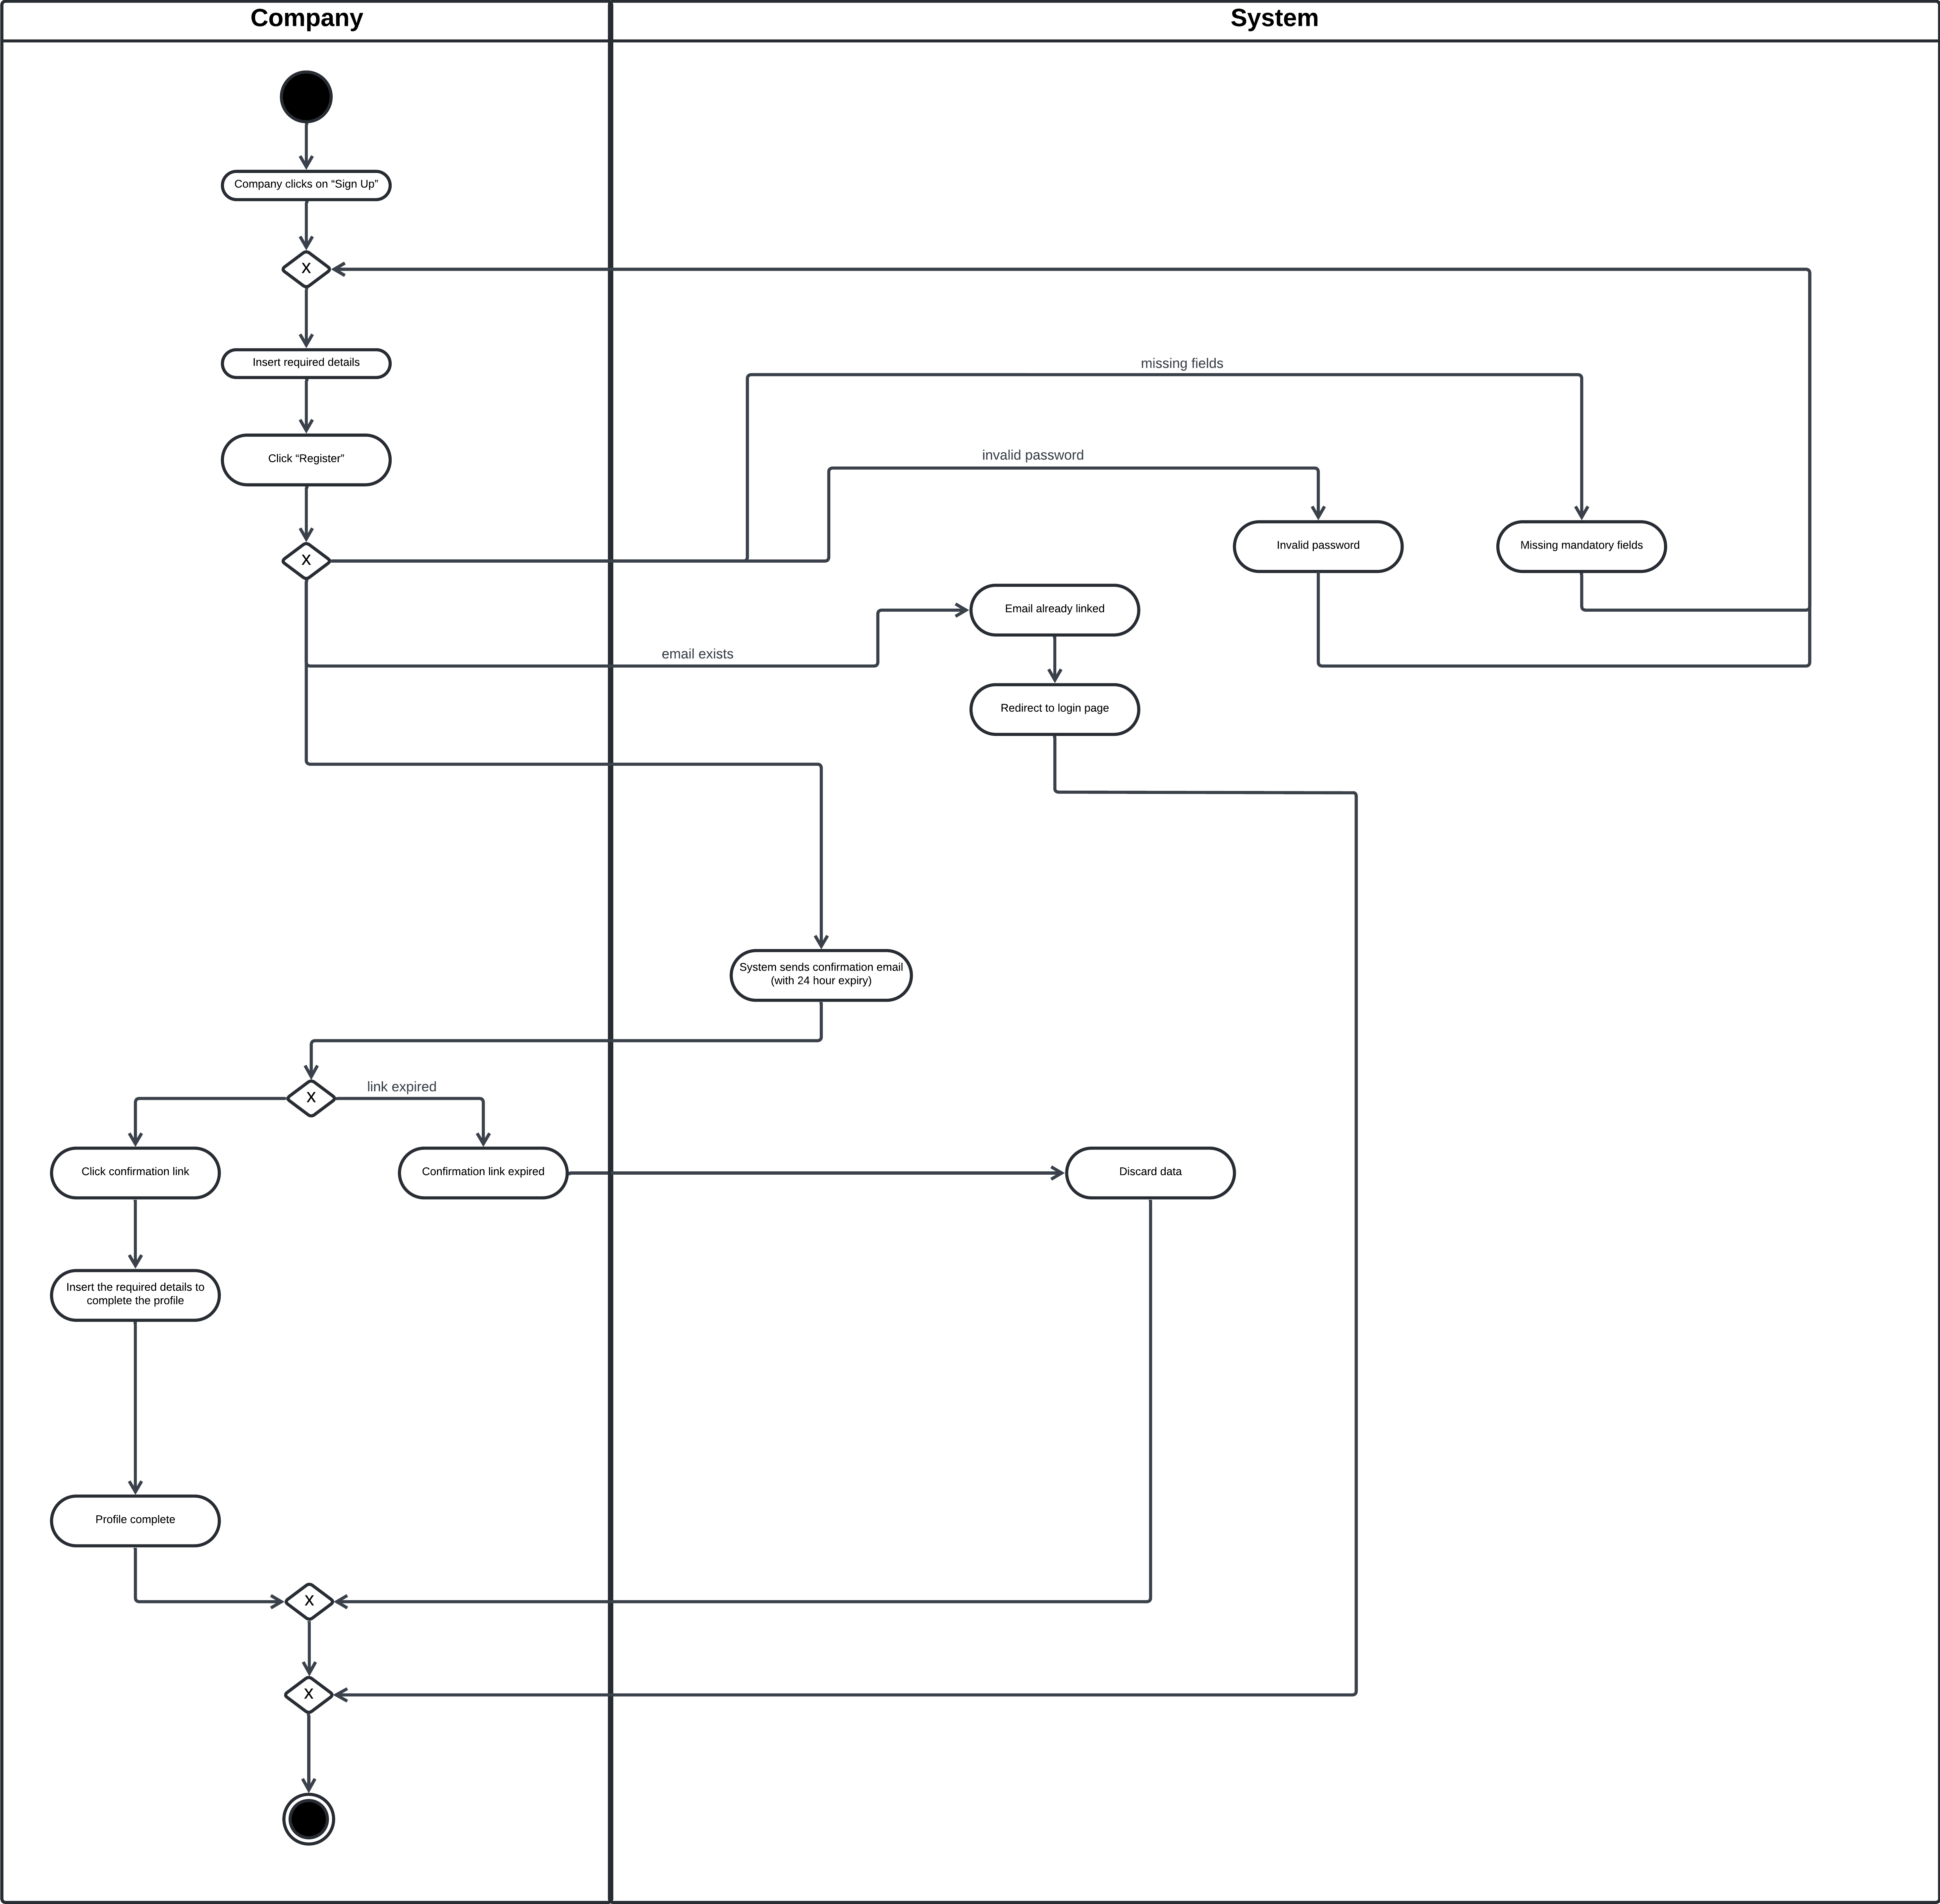
\includegraphics[width=1\linewidth]{LaTeXCode/images/activity diagram/UC2.png}
         \caption{Sign Up by a Company}
         \label{fig:signup_company_ad}
     \end{center}
\end{figure}

\newpage

\subsubsection*{UC\cuc . Sign Up by a University}
\begin{center}
    \begin{longtable}{|l|p{0.75\linewidth}|}
        \hline
        \textbf{Actor}            & University\\
        \hline
        \textbf{Entry Conditions} & The University is not logged into the S\&C platform. \\
        \hline
        \textbf{Flow of Events}       
        & \cucsteps. On the homepage, the University clicks the "Sign Up" button, entering the companies' registration page. \\
        & \cucsteps. The University provides the required details: User category (University), email, password and password confirmation. \\
        & \cucsteps. The University confirms the provided information by clicking the "Register" button. \\
        & \cucsteps. The system sends to the indicated mailbox a confirmation email with a link that expires in 24 hours for account verification purposes. \\
        & \cucsteps. The University clicks the link in the confirmation email and logs into the platform. \\
        & \cucsteps. On the profile page, the University completes the university's profile by adding relevant details: university name, location, phone number, faculties, key contacts for internships, university website. \\
        \hline
        \textbf{Exit Conditions}   & The profile is complete and the University has access to all its functionalities. \\       
        \hline
        \textbf{Exceptions}       & \begin{itemize}
            \item The email address is already linked to an existing account: an error message is shown, and the University is redirected to the login page.
            \item The password does not meet the platform security requirements: An error message is displayed, and the University is required to correct the password.
            \item Some mandatory fields are missing: the system does not allow the University to complete the procedure until all the mandatory fields are filled out.
            \item The confirmation link sent to the indicated mailbox expires: all information previously inserted into the system by the University is discarded and the link is invalidated.
        \end{itemize}\\
        \hline
    \end{longtable}
\end{center}

\begin{figure}[H]
    \begin{center}
         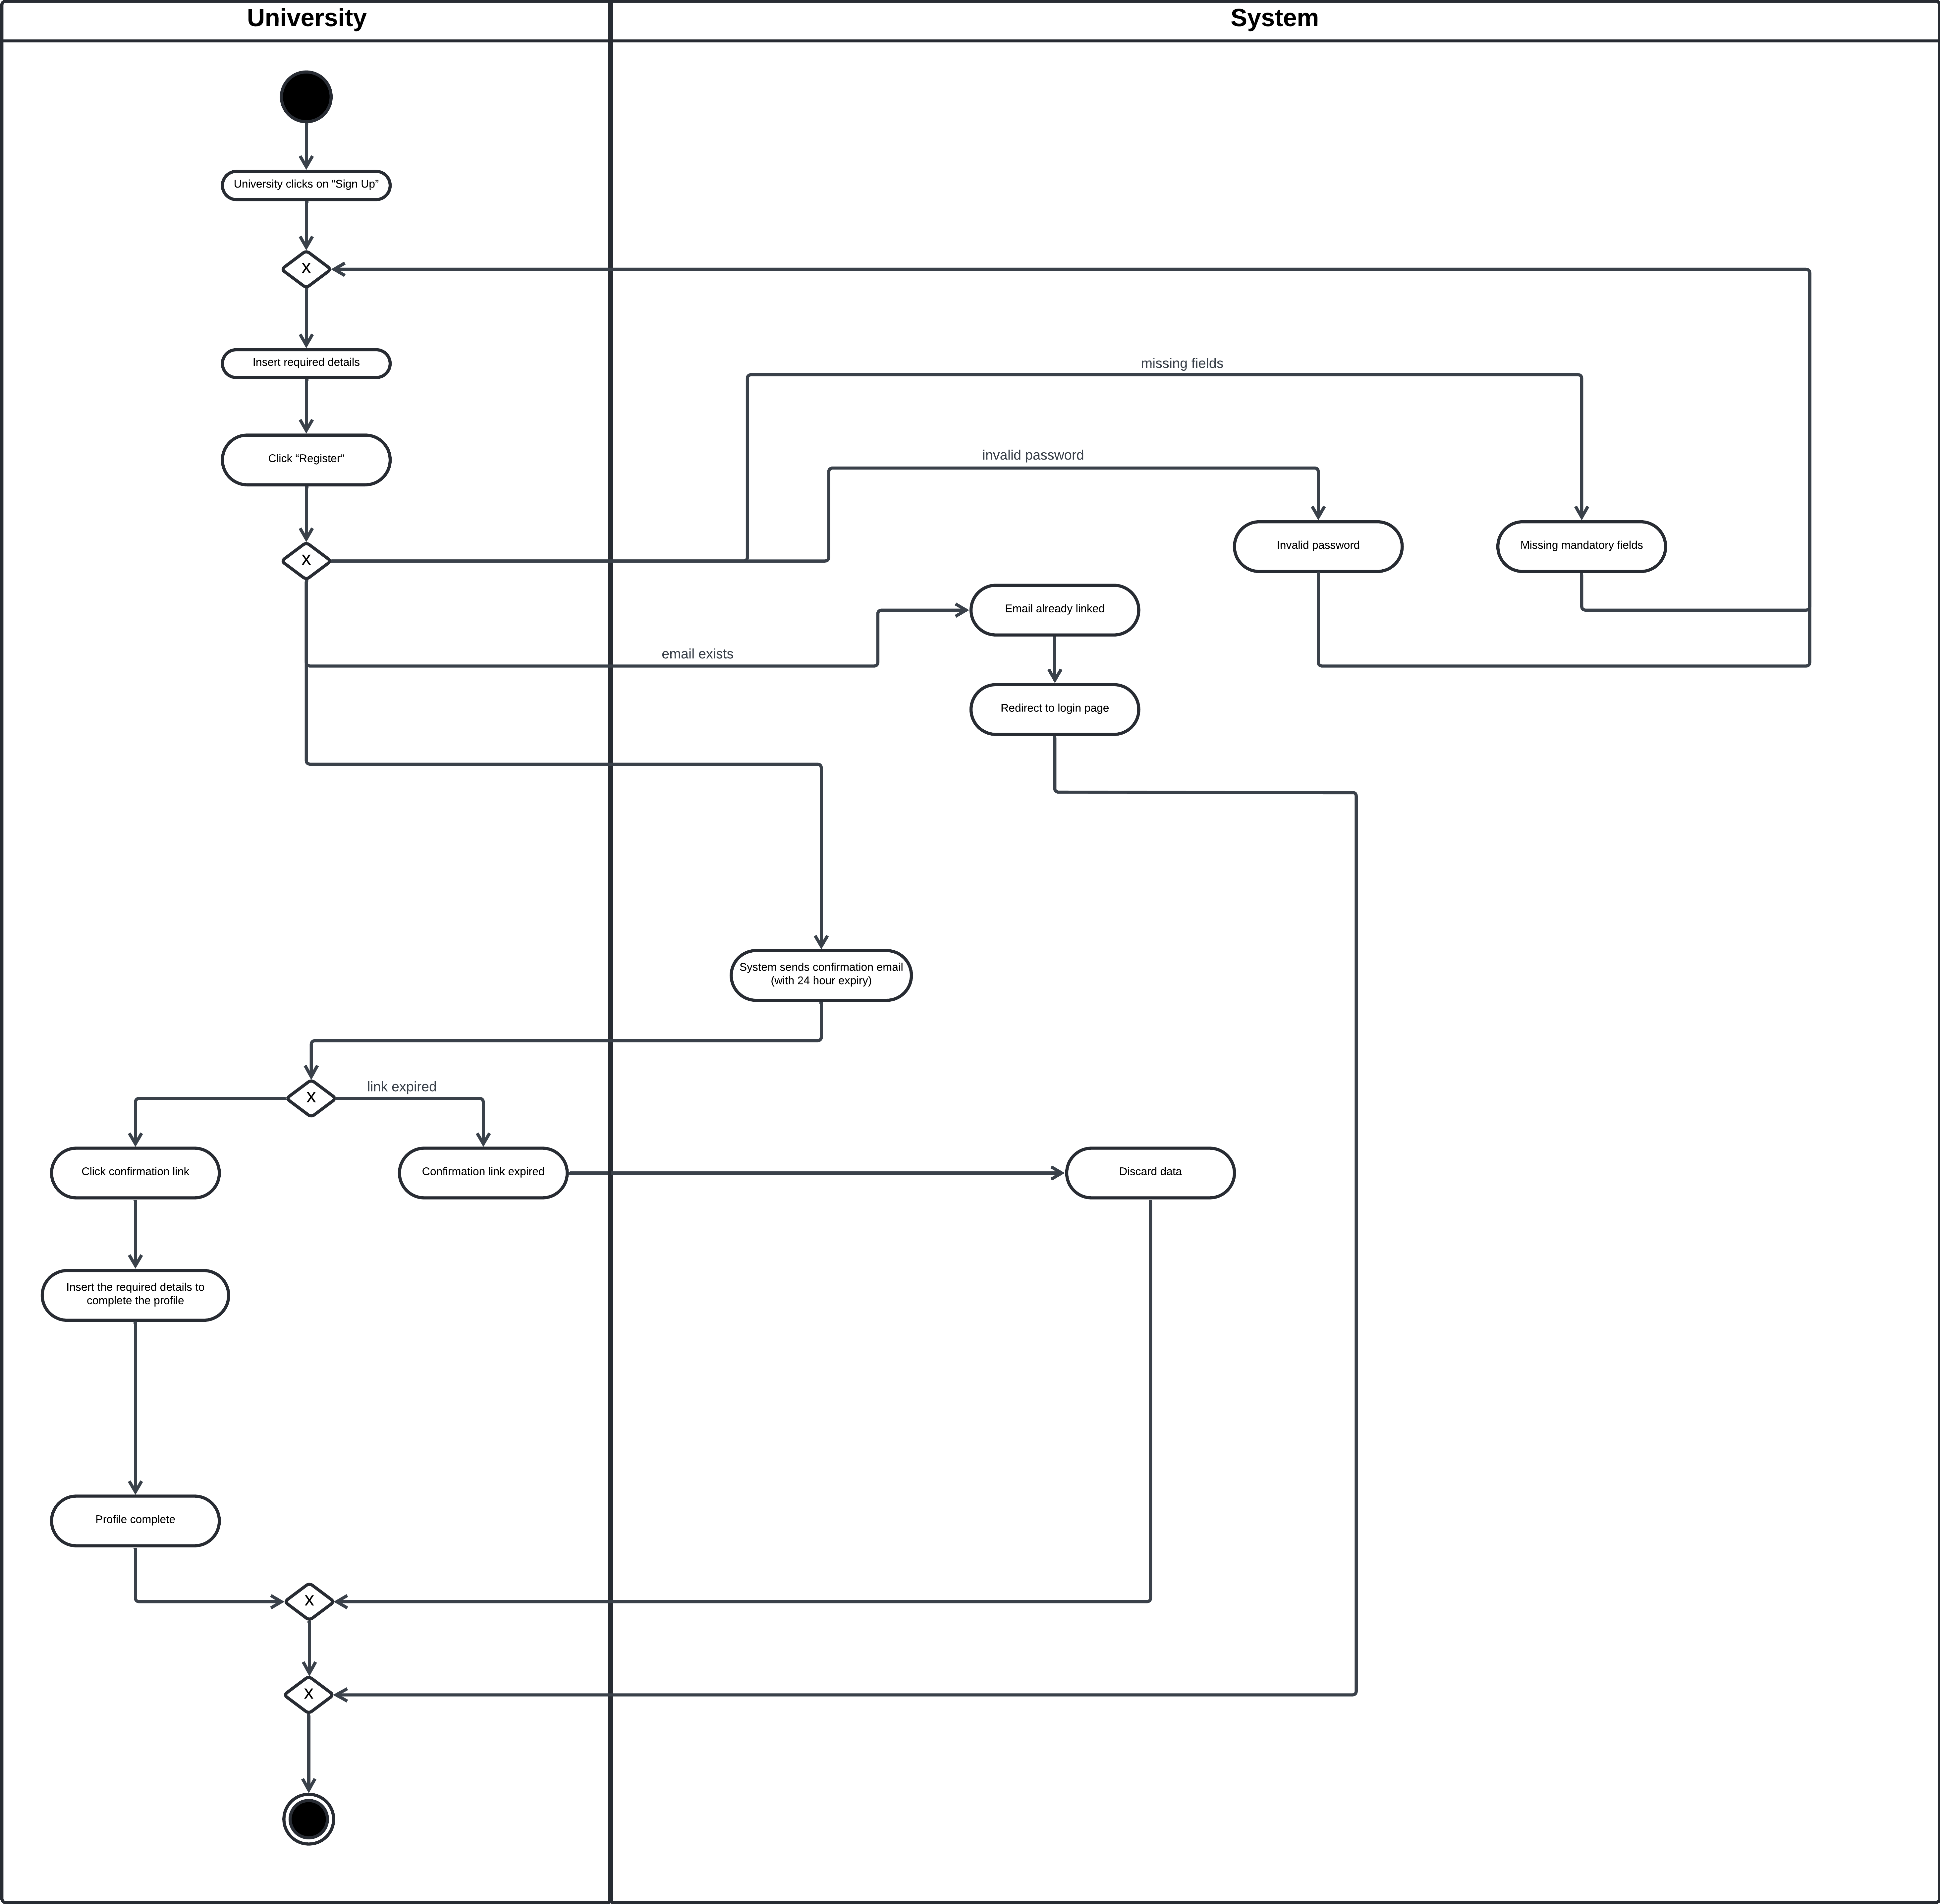
\includegraphics[width=1\linewidth]{LaTeXCode/images/activity diagram/UC3.png}
         \caption{Sign Up by a University}
         \label{fig:signup_university_ad}
     \end{center}
\end{figure}

\newpage

\subsubsection*{UC\cuc . Log In by a User}
\begin{center}
    \begin{longtable}{|l|p{0.75\linewidth}|}
        \hline
        \textbf{Actor}            & User (Student, Company or University) \\
        \hline
        \textbf{Entry Conditions} & The User is not already logged into the S\&C platform. \\
        \hline
        \textbf{Flow of Events}       
        & \cucsteps. On the homepage, the User clicks the "Login" button, which displays the login form. \\
        & \cucsteps. The User enters their email and password into the designated fields. \\
        & \cucsteps. The User clicks the "Login" button. \\
        & \cucsteps. The system validates the provided credentials. \\
        & \cucsteps. The system redirects the User to the dashboard page. \\
        \hline
        \textbf{Exit Conditions}   & The User is successfully logged in. \\       
        \hline
        \textbf{Exceptions}       & \begin{itemize}
            \item The inserted credentials are incorrect: the system displays an error message indicating that the credentials are invalid and the User remains on the login page.
            \item The account hasn't been verified yet: if the User has not confirmed their email and the confirmation link has not expired yet, the system shows a message requesting to complete the verification process.
            \item The profile of the logged User is incomplete: the User is redirected to the Update Profile page instead of the dashboard page.
        \end{itemize}\\
        \hline
    \end{longtable}
\end{center}

\begin{figure}[H]
    \begin{center}
         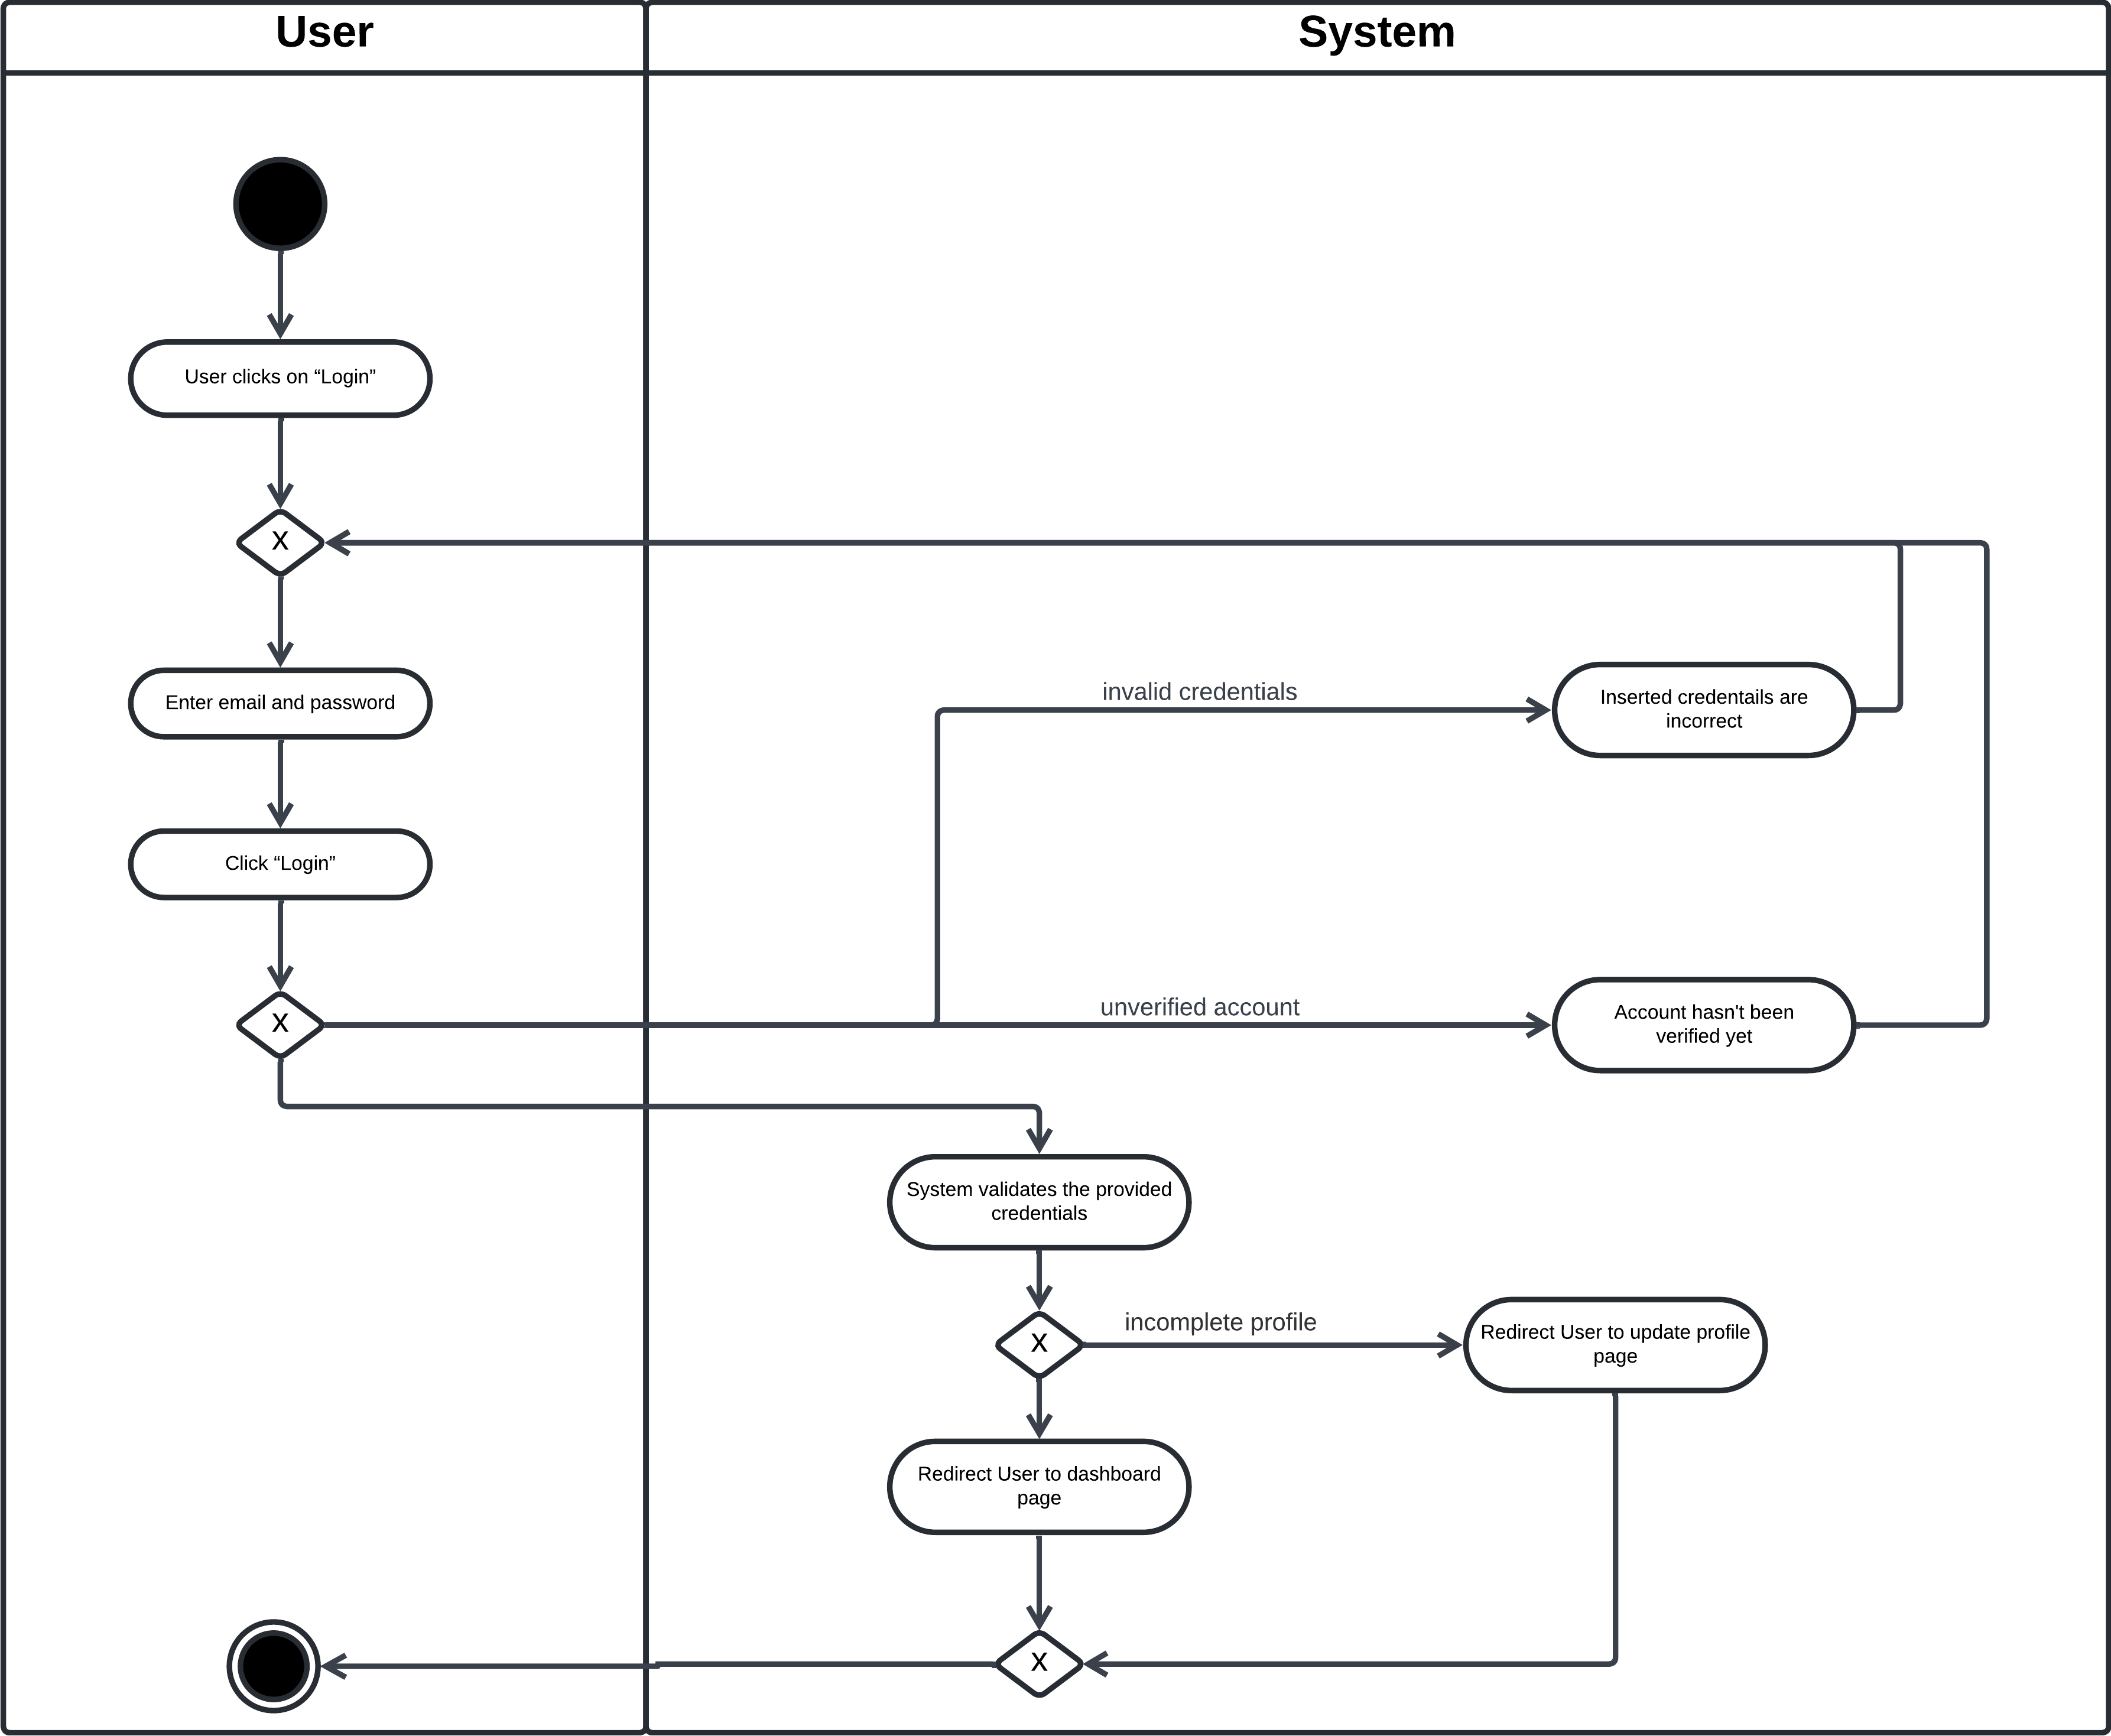
\includegraphics[width=1\linewidth]{LaTeXCode/images/activity diagram/UC4.png}
         \caption{Login by a User}
         \label{fig:login_user_ad}
     \end{center}
\end{figure}

\newpage

\subsubsection*{UC\cuc . Update User Profile}
\begin{center}
    \begin{longtable}{|l|p{0.75\linewidth}|}
        \hline
        \textbf{Actor}            & User\\
        \hline
        \textbf{Entry Conditions} & The User is logged into the S\&C platform.\\
        \hline
        \textbf{Flow of Events}   
        & \cucsteps. In their "Profile" section, the User clicks the "Edit" button. \\ 
        & \cucsteps. The User updates the desired details of its profile. \\
        & \cucsteps. The User confirms the applied changes by clicking the \newline "Apply Changes" button. \\
        & \cucsteps. If the User is a Student and the updated details are relevant, the system starts an instance of the process for identifying new recommendations via the \hyperref[subsec: generate_recommendations_uc]{\uline{UC. Generate Recommendations}} functionality. \\
        \hline
        \textbf{Exit Conditions}   & The User's profile is updated and its changes are recorded in the system. \\    
        \hline
        \textbf{Exceptions}       & \begin{itemize}
            \item Some mandatory fields are left empty: the system doesn't allow the User to complete the procedure until all the mandatory fields are filled out.
        \end{itemize}\\
        \hline
    \end{longtable}
\end{center}
\label{subsec: update_profile_uc}

\begin{figure}[H]
    \begin{center}
         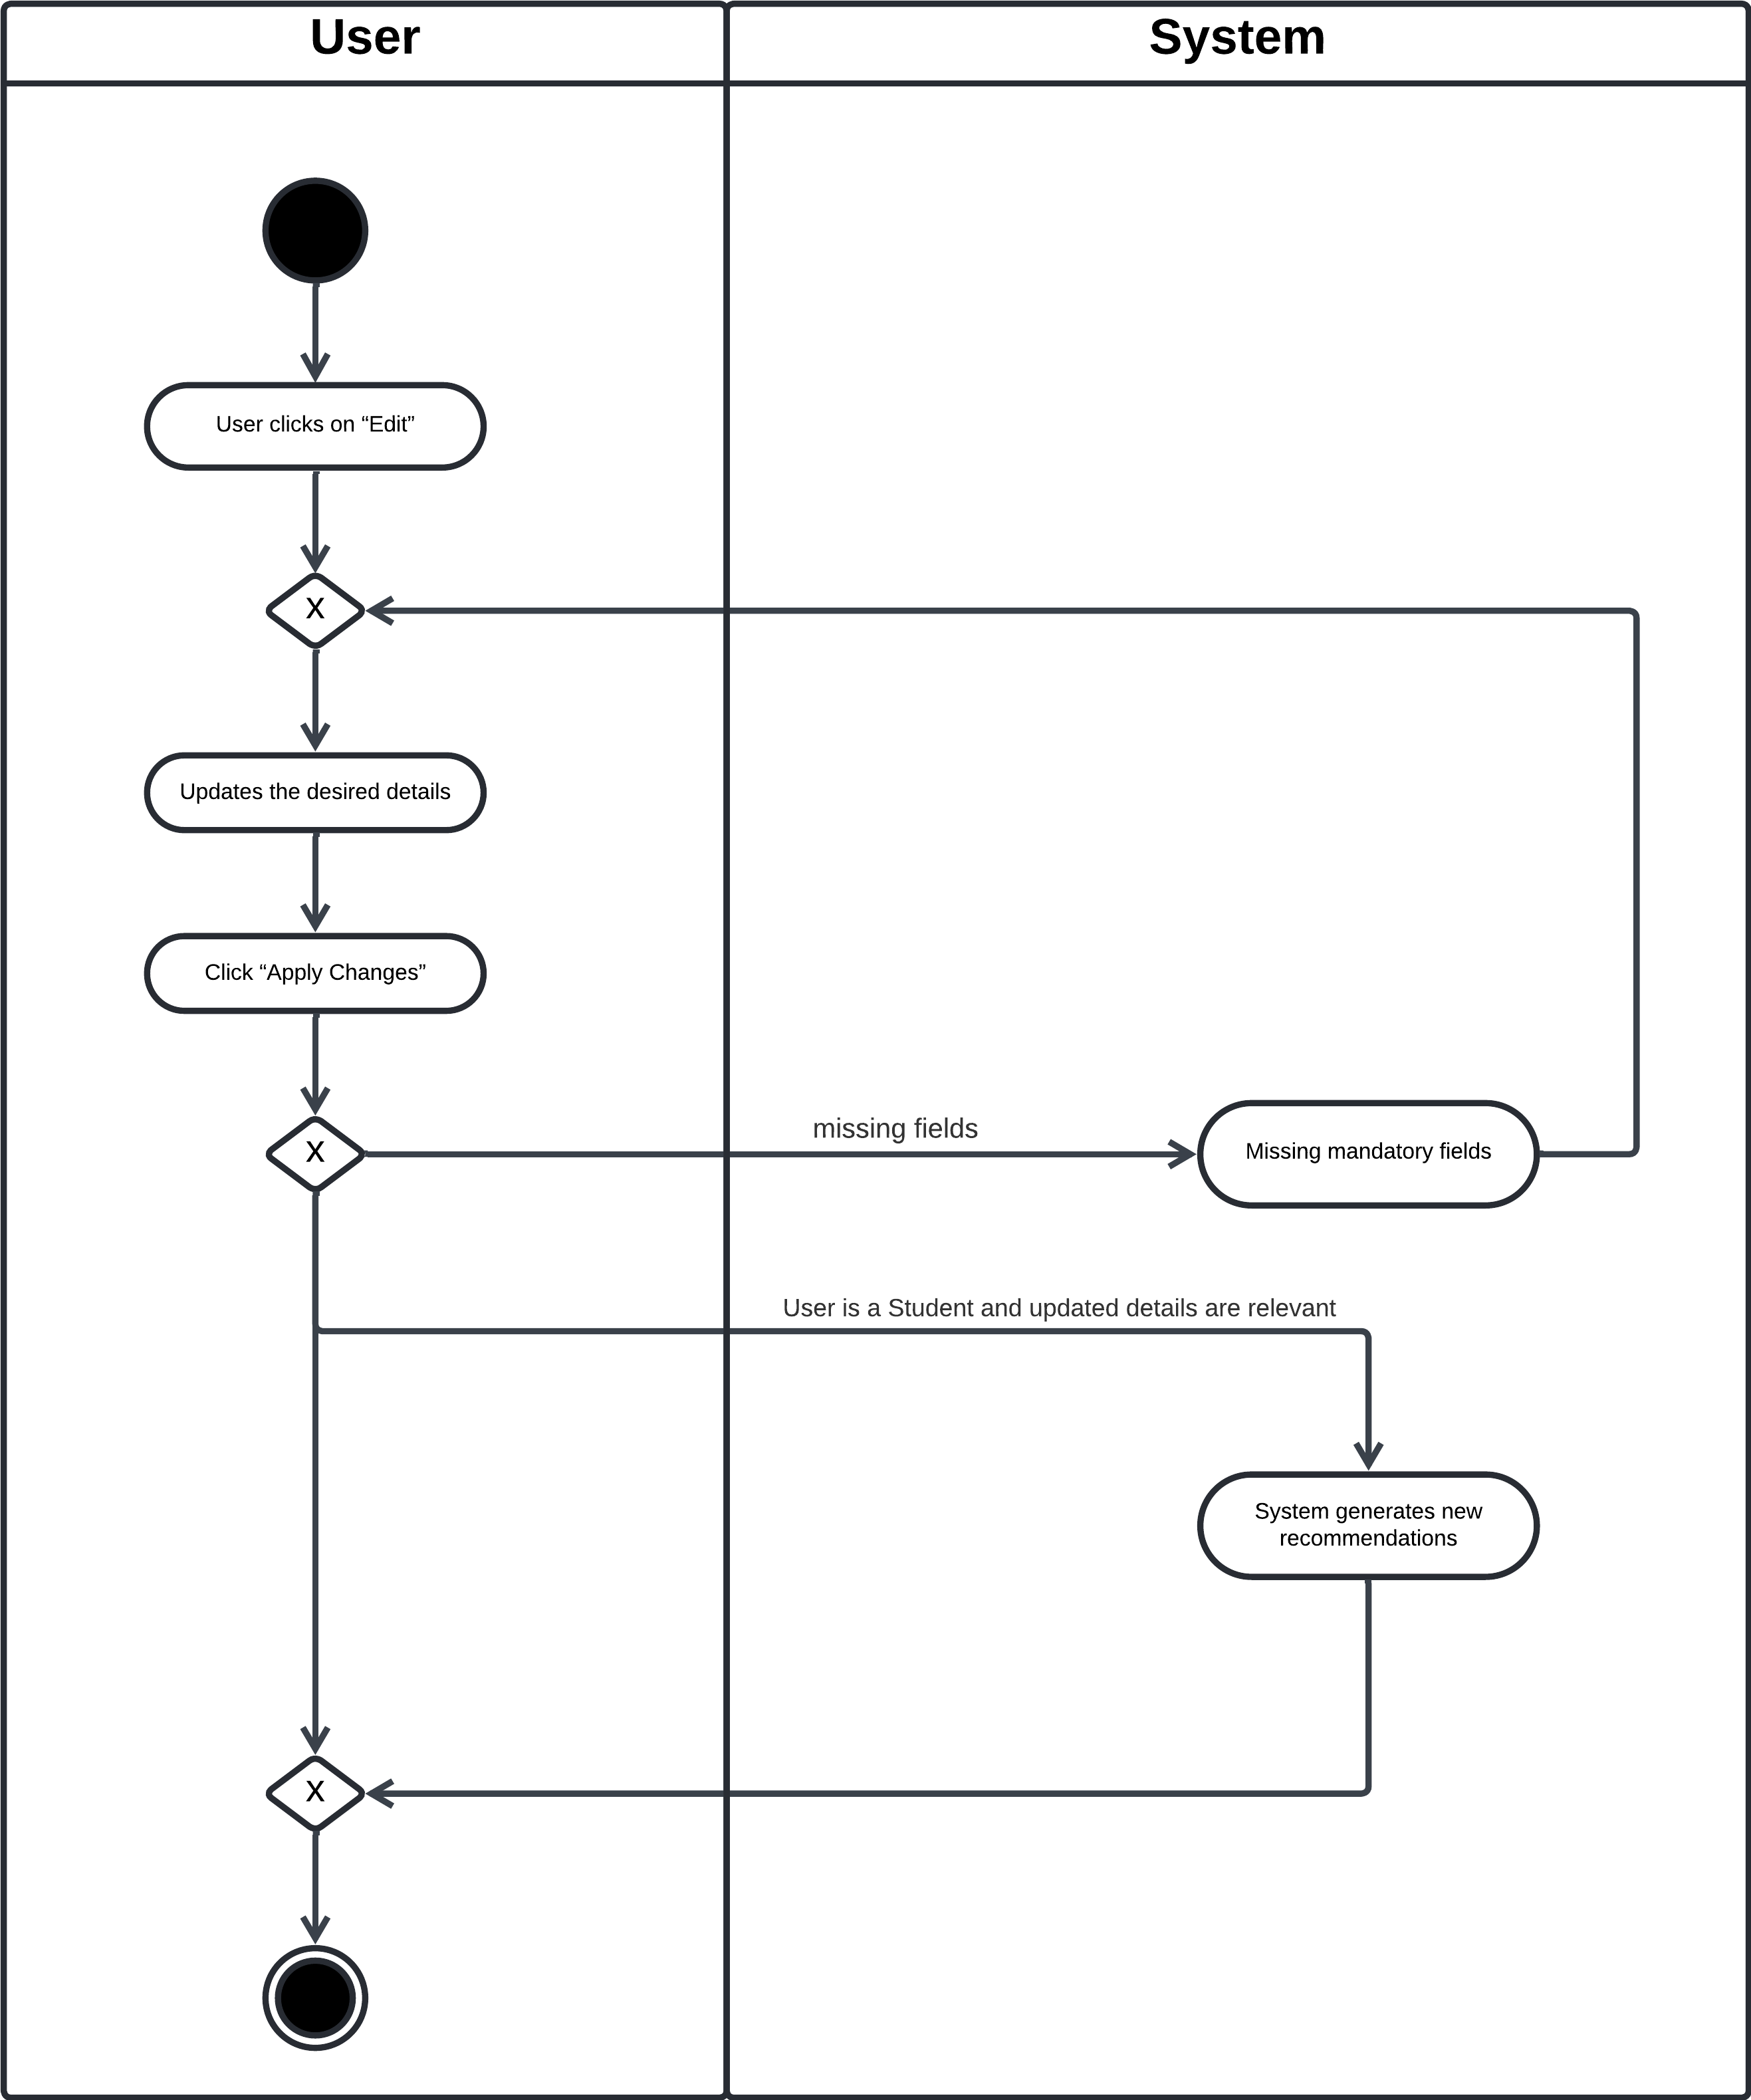
\includegraphics[width=1\linewidth]{LaTeXCode/images/activity diagram/UC5.png}
         \caption{Update User profile}
         \label{fig:update_profile_ad}
     \end{center}
\end{figure}

\newpage

\subsubsection*{UC\cuc . Publish an Internship Offer}
\begin{center}
    \begin{longtable}{|l|p{0.75\linewidth}|}
        \hline
        \textbf{Actor}            & Company \\
        \hline
        \textbf{Entry Conditions} & The Company is logged into the S\&C platform. \\
        \hline
        \textbf{Flow of Events}       
        & \cucsteps. In the dashboard, the Company clicks the "Create New Offer" button, entering the internship creation page. \\
        & \cucsteps. The Company fills out the internship creation form, inserting:
        \begin{itemize}
            \item Position
            \item Tasks to be performed
            \item Required skills
            \item Internship duration
            \item Compensation terms 
            \item Location (on-site, hybrid, or remote)
            \item Application deadline
        \end{itemize}\\
        & \cucsteps. The Company clicks the "Submit" button, waiting for the automatic data verification. \\
        & \cucsteps. The system verifies the provided data to ensure the provided information is compliant with platform guidelines, and the data is consistent and accurate. \\
        & \cucsteps. The system publishes the internship offer on the platform, making it visible to all students. \\
        & \cucsteps. The system confirms to the Company that its offer has been published. \\
        & \cucsteps. If the updated details are relevant, the system starts an instance of the process for identifying new recommendations via the \hyperref[subsec: generate_recommendations_uc]{\uline{UC. Generate Recommendations}} functionality. \\
        \hline
        \textbf{Exit Conditions}   & The internship offer is published on the platform and accessible to students. \\       
        \hline
        \textbf{Exceptions}       & \begin{itemize}
            \item Some mandatory fields are missing: the system doesn’t allow the Company to complete the procedure until all the mandatory fields are filled out.
            \item Some information is not compliant with platform guidelines: the system alerts the Company about the issue and requires revisions.
        \end{itemize} \\
        \hline
    \end{longtable}
\end{center}

\begin{figure}[H]
    \begin{center}
         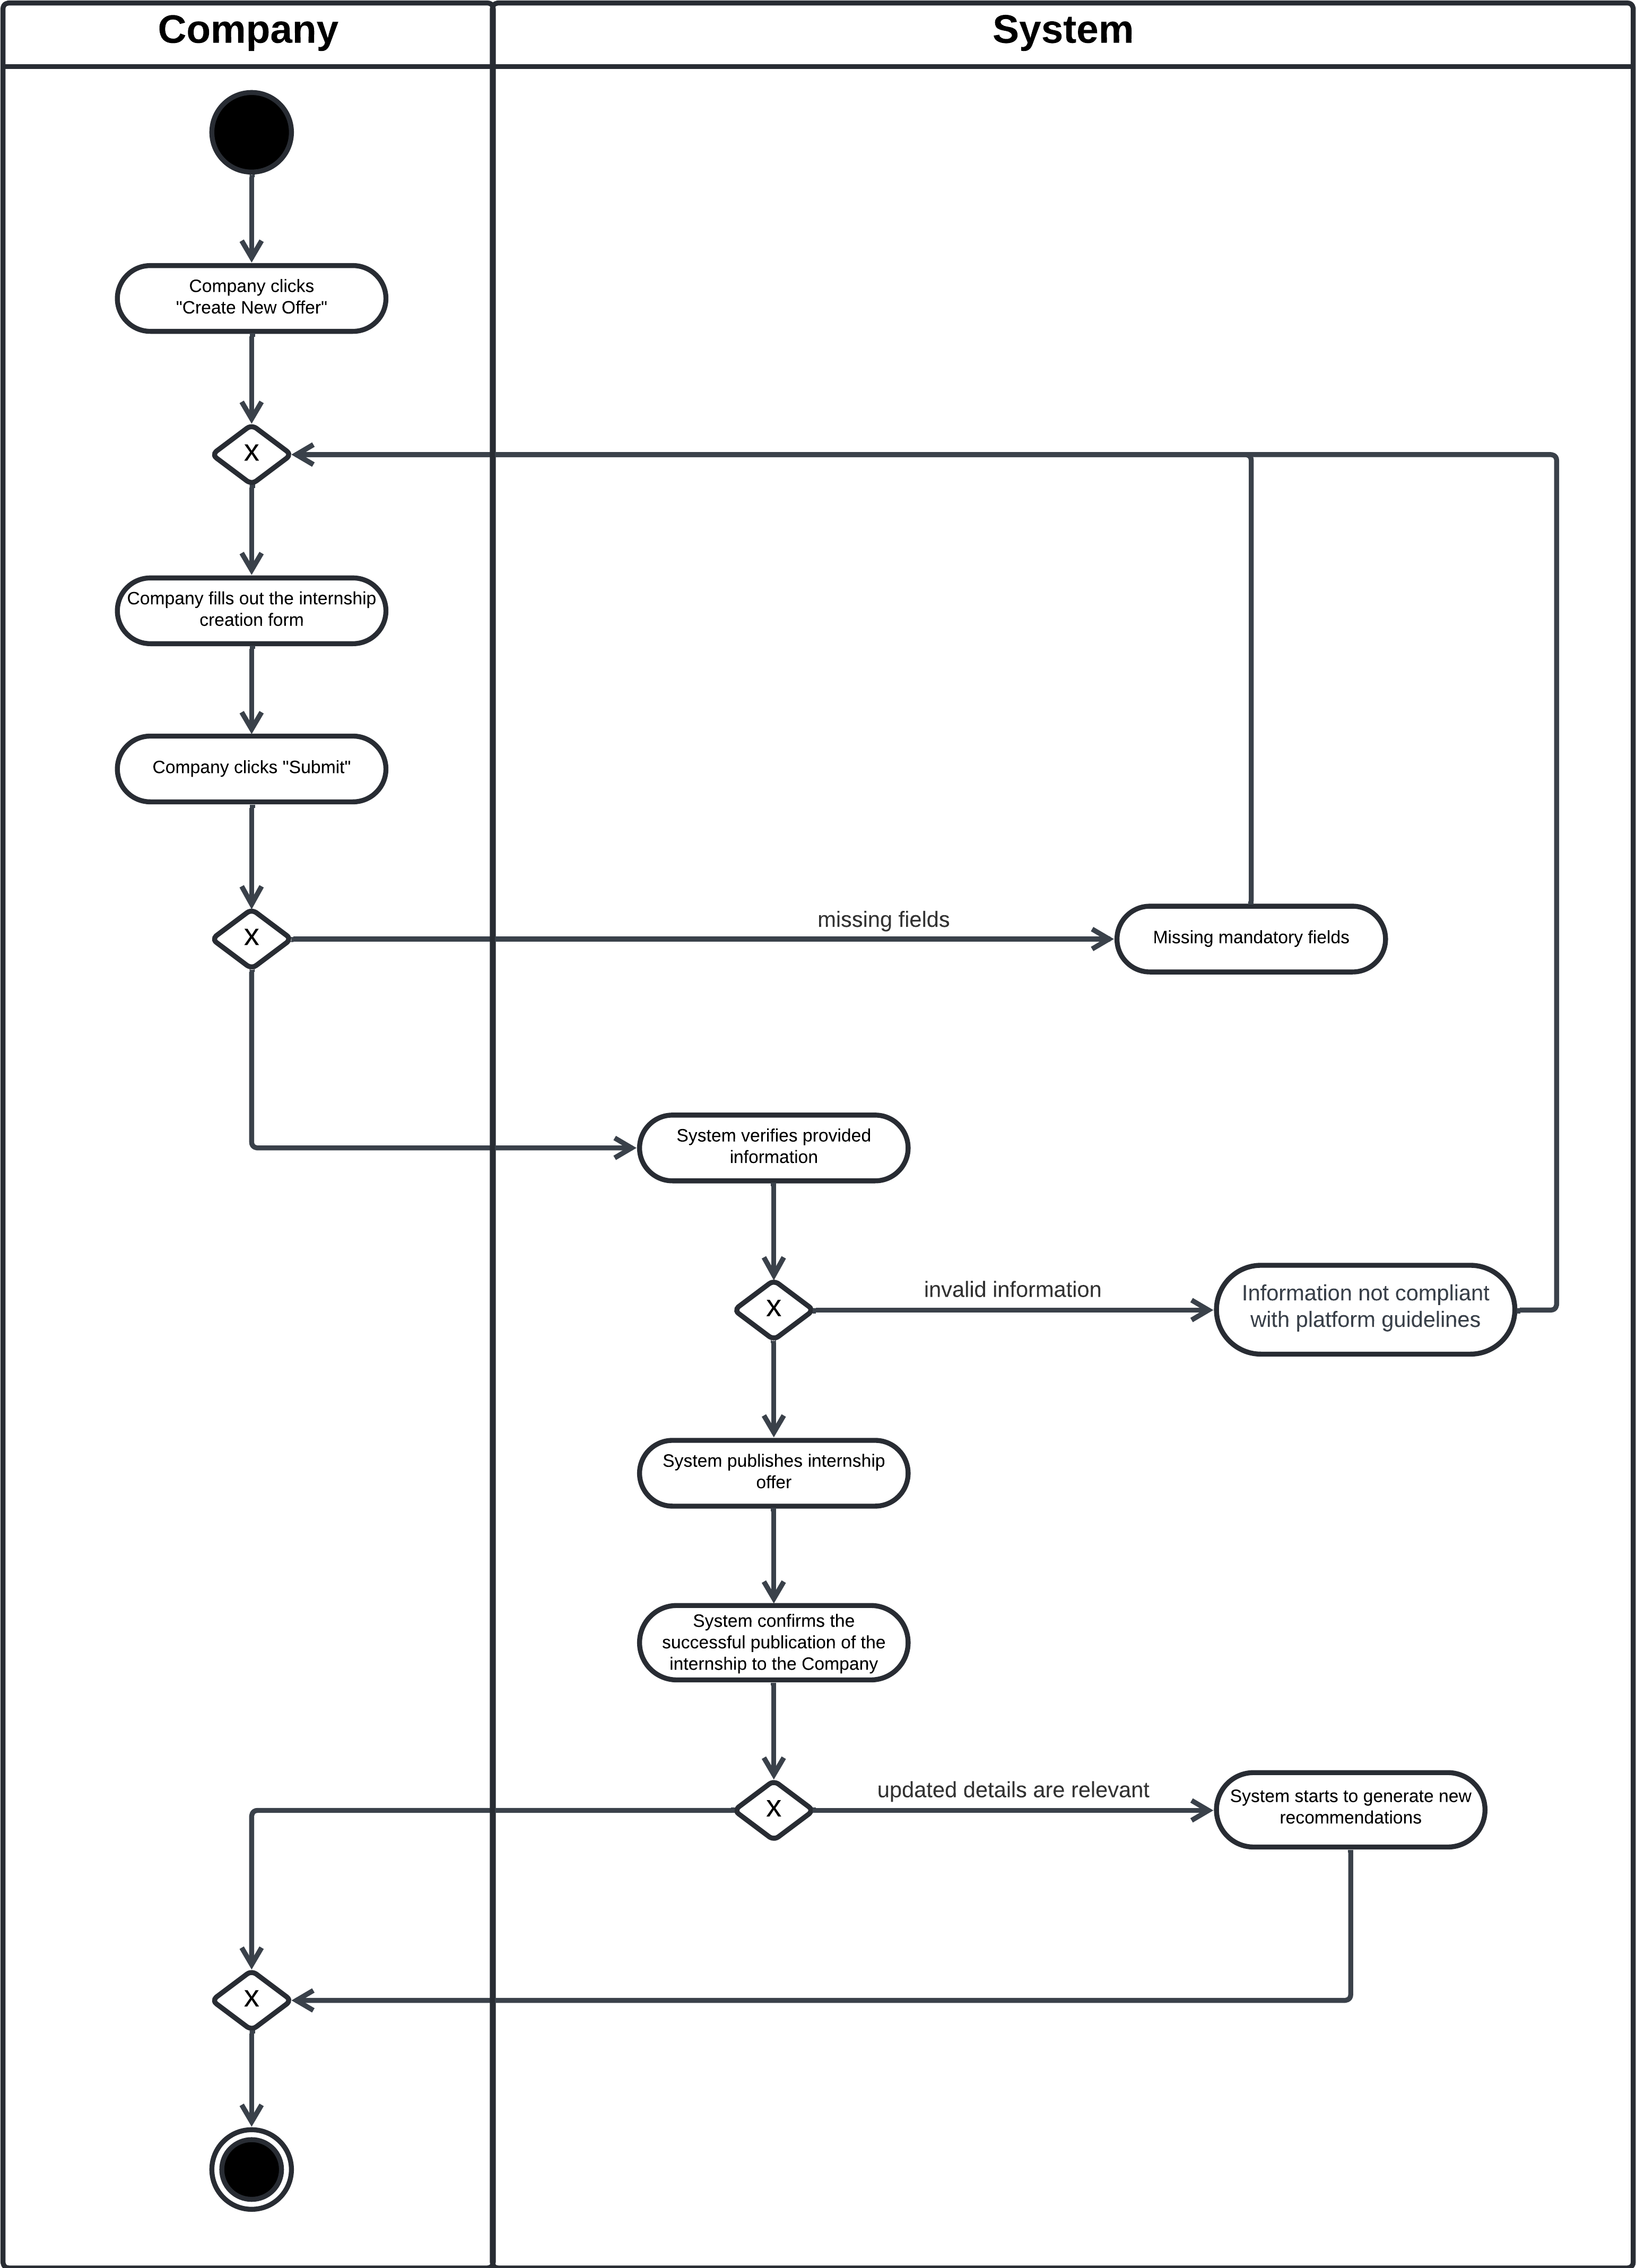
\includegraphics[width=1\linewidth]{LaTeXCode/images/activity diagram/UC6.png}
         \caption{Publish an Internship Offer}
         \label{fig:publish_offer_ad}
     \end{center}
\end{figure}

\newpage

\subsubsection*{UC\cuc . Update Internship Offer}
\begin{center}
    \begin{longtable}{|l|p{0.75\linewidth}|}
        \hline
        \textbf{Actor}            & Company\\
        \hline
        \textbf{Entry Conditions} & The Company is logged into the S\&C platform and the selected internship offer’s application deadline has not expired yet.\\
        \hline
        \textbf{Flow of Events}   
        & \cucsteps. On the selected internship offer's page, the Company clicks the "Edit" button. \\ 
        & \cucsteps. The Company updates the desired details of the internship offer or chooses to withdraw it entirely by clicking the "Withdraw Offer" button. \\
        & \theucsteps. The Company acts accordingly based on their decision: \\
        & \theucsteps.1. If the Company updates the details, it confirms the applied changes by clicking the "Apply Changes" button. \\
        & \cucsteps.2. If the Company chooses to withdraw the offer, a confirmation prompt appears, asking to finalize the withdrawal. Upon confirmation, the internship offer is marked as "Closed" and becomes inaccessible to students. \\
        & \theucsteps.1. If updates are confirmed, the system records the changes. \\
        & \cucsteps.2. If the offer is withdrawn, the system cancels all pending processes related to the offer, such as identifying new recommendations or managing applications. \\
        & \cucsteps. For an updated offer, the system starts an instance of the process for identifying new recommendations via the \hyperref[subsec: generate_recommendations_uc]{\uline{UC. Generate Recommendations}} functionality. \\
        \hline
        \textbf{Exit Conditions}   & The selected internship offer is updated and its changes are recorded in the system. \\    
        \hline
        \textbf{Exceptions}       & \begin{itemize}
            \item Some mandatory fields are missing: the system doesn't allow the Company to complete the procedure until all the mandatory fields are filled out.
            \item Some information is not compliant with platform guidelines: the system alerts the Company about the issue and requires revisions.
        \end{itemize}\\
        \hline
    \end{longtable}
\end{center}
\label{subsec: update_internship_offer_uc}

\begin{figure}[H]
    \begin{center}
         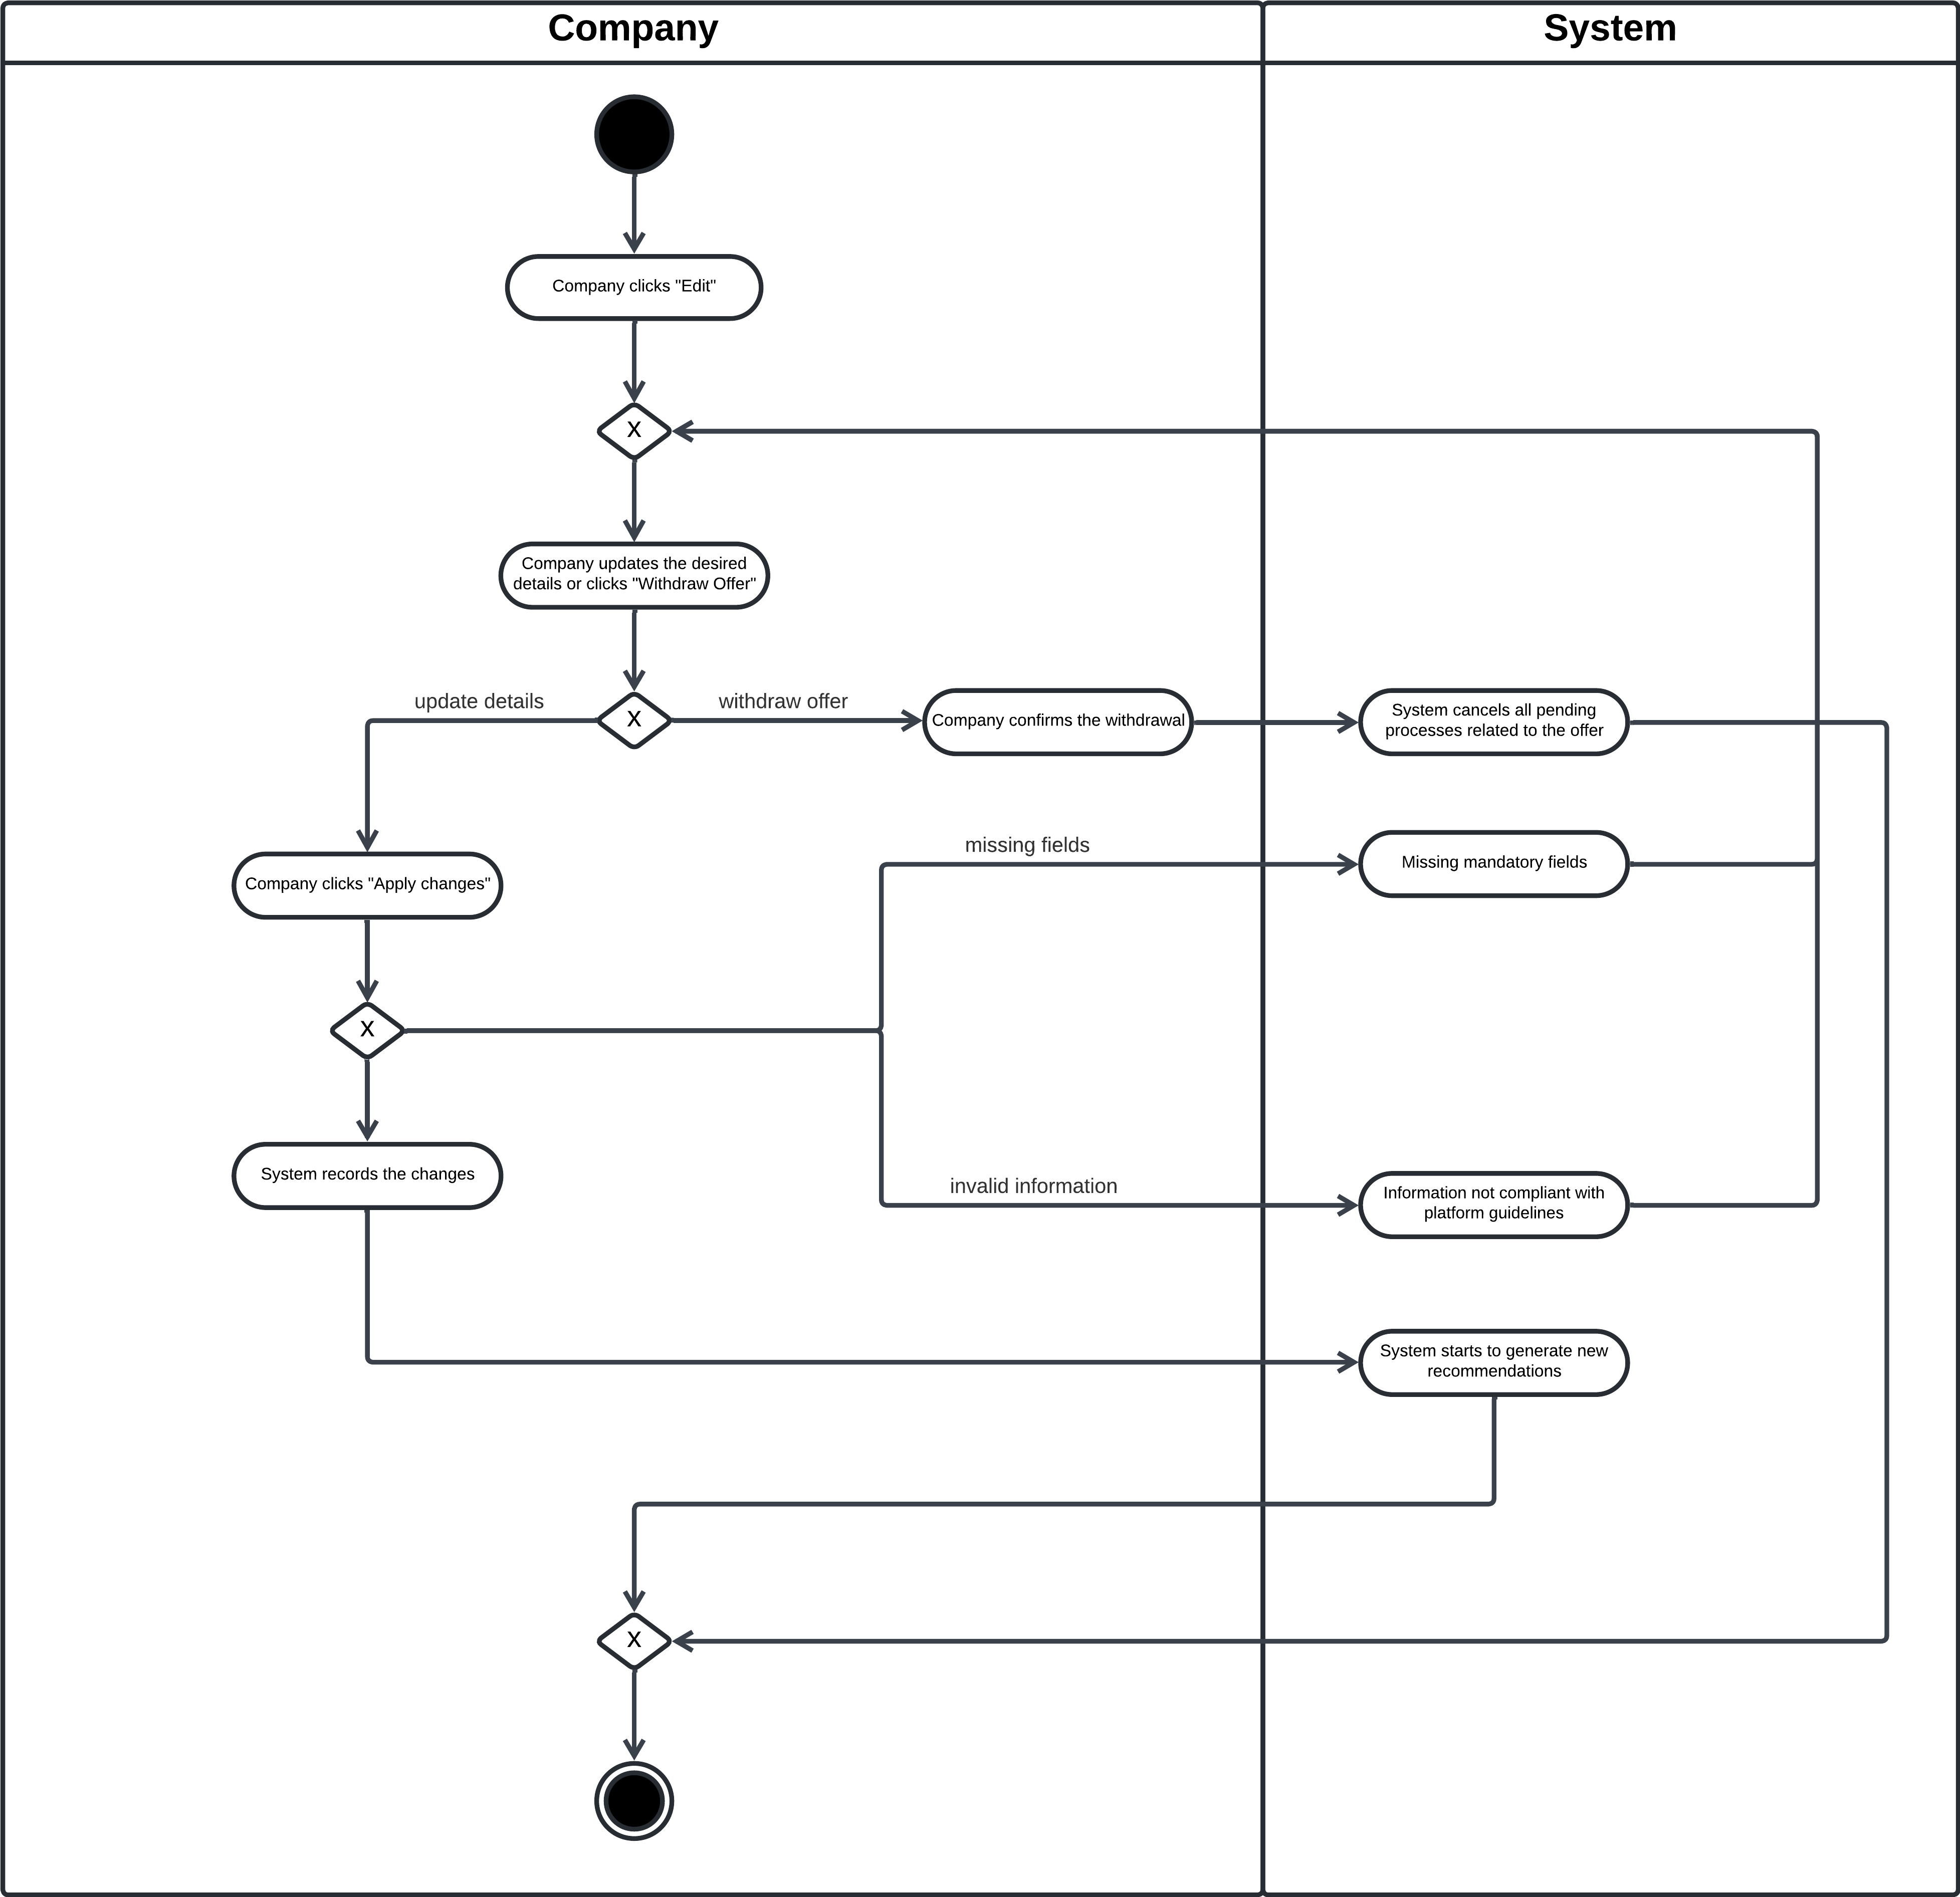
\includegraphics[width=1\linewidth]{LaTeXCode/images/activity diagram/UC7.png}
         \caption{Update Internship Offer}
         \label{fig:update_internship_offer_ad}
     \end{center}
\end{figure}

\newpage

\subsubsection*{UC\cuc . Search Internship Offers}
\begin{center}
    \begin{longtable}{|l|p{0.75\linewidth}|}
        \hline
        \textbf{Actor}            & Student \\
        \hline
        \textbf{Entry Conditions} & The Student is logged into the S\&C platform. \\
        \hline
        \textbf{Flow of Events}       
        & \cucsteps. In the dashboard, the Student navigates to the "Search Offers" section. \\
        & \cucsteps. The system displays a search interface which has the following optional filters:
        \begin{itemize}
            \item Domain of interest
            \item Location (on-site, hybrid, or remote)
            \item Internship duration
            \item Compensation terms
            \item Keywords (an offer matches a keyword if it contains that keyword or a semantically similar one in any of its fields).
        \end{itemize}\\
        & \cucsteps. The Student selects the desired filters and submits the query to the system. \\
        & \cucsteps. The system retrieves and displays a list of internship offers that match the selected criteria. \\
        & \cucsteps. Optionally, the Student applies one or more ordering criteria: newest, oldest, most relevant, or most number of applications, by selecting the desired ones from a drop-down list. \\
        \hline
        \textbf{Exit Conditions}   & The system displays the list of internship offers matching the given criteria. \\ 
        \hline
        \textbf{Exceptions}       & \begin{itemize}
            \item The system doesn't find any matching result: if none of the active internship offers matches the selected criteria, the system displays a message indicating it.
        \end{itemize}\\
        \hline
    \end{longtable}
\end{center}

\begin{figure}[H]
    \begin{center}
         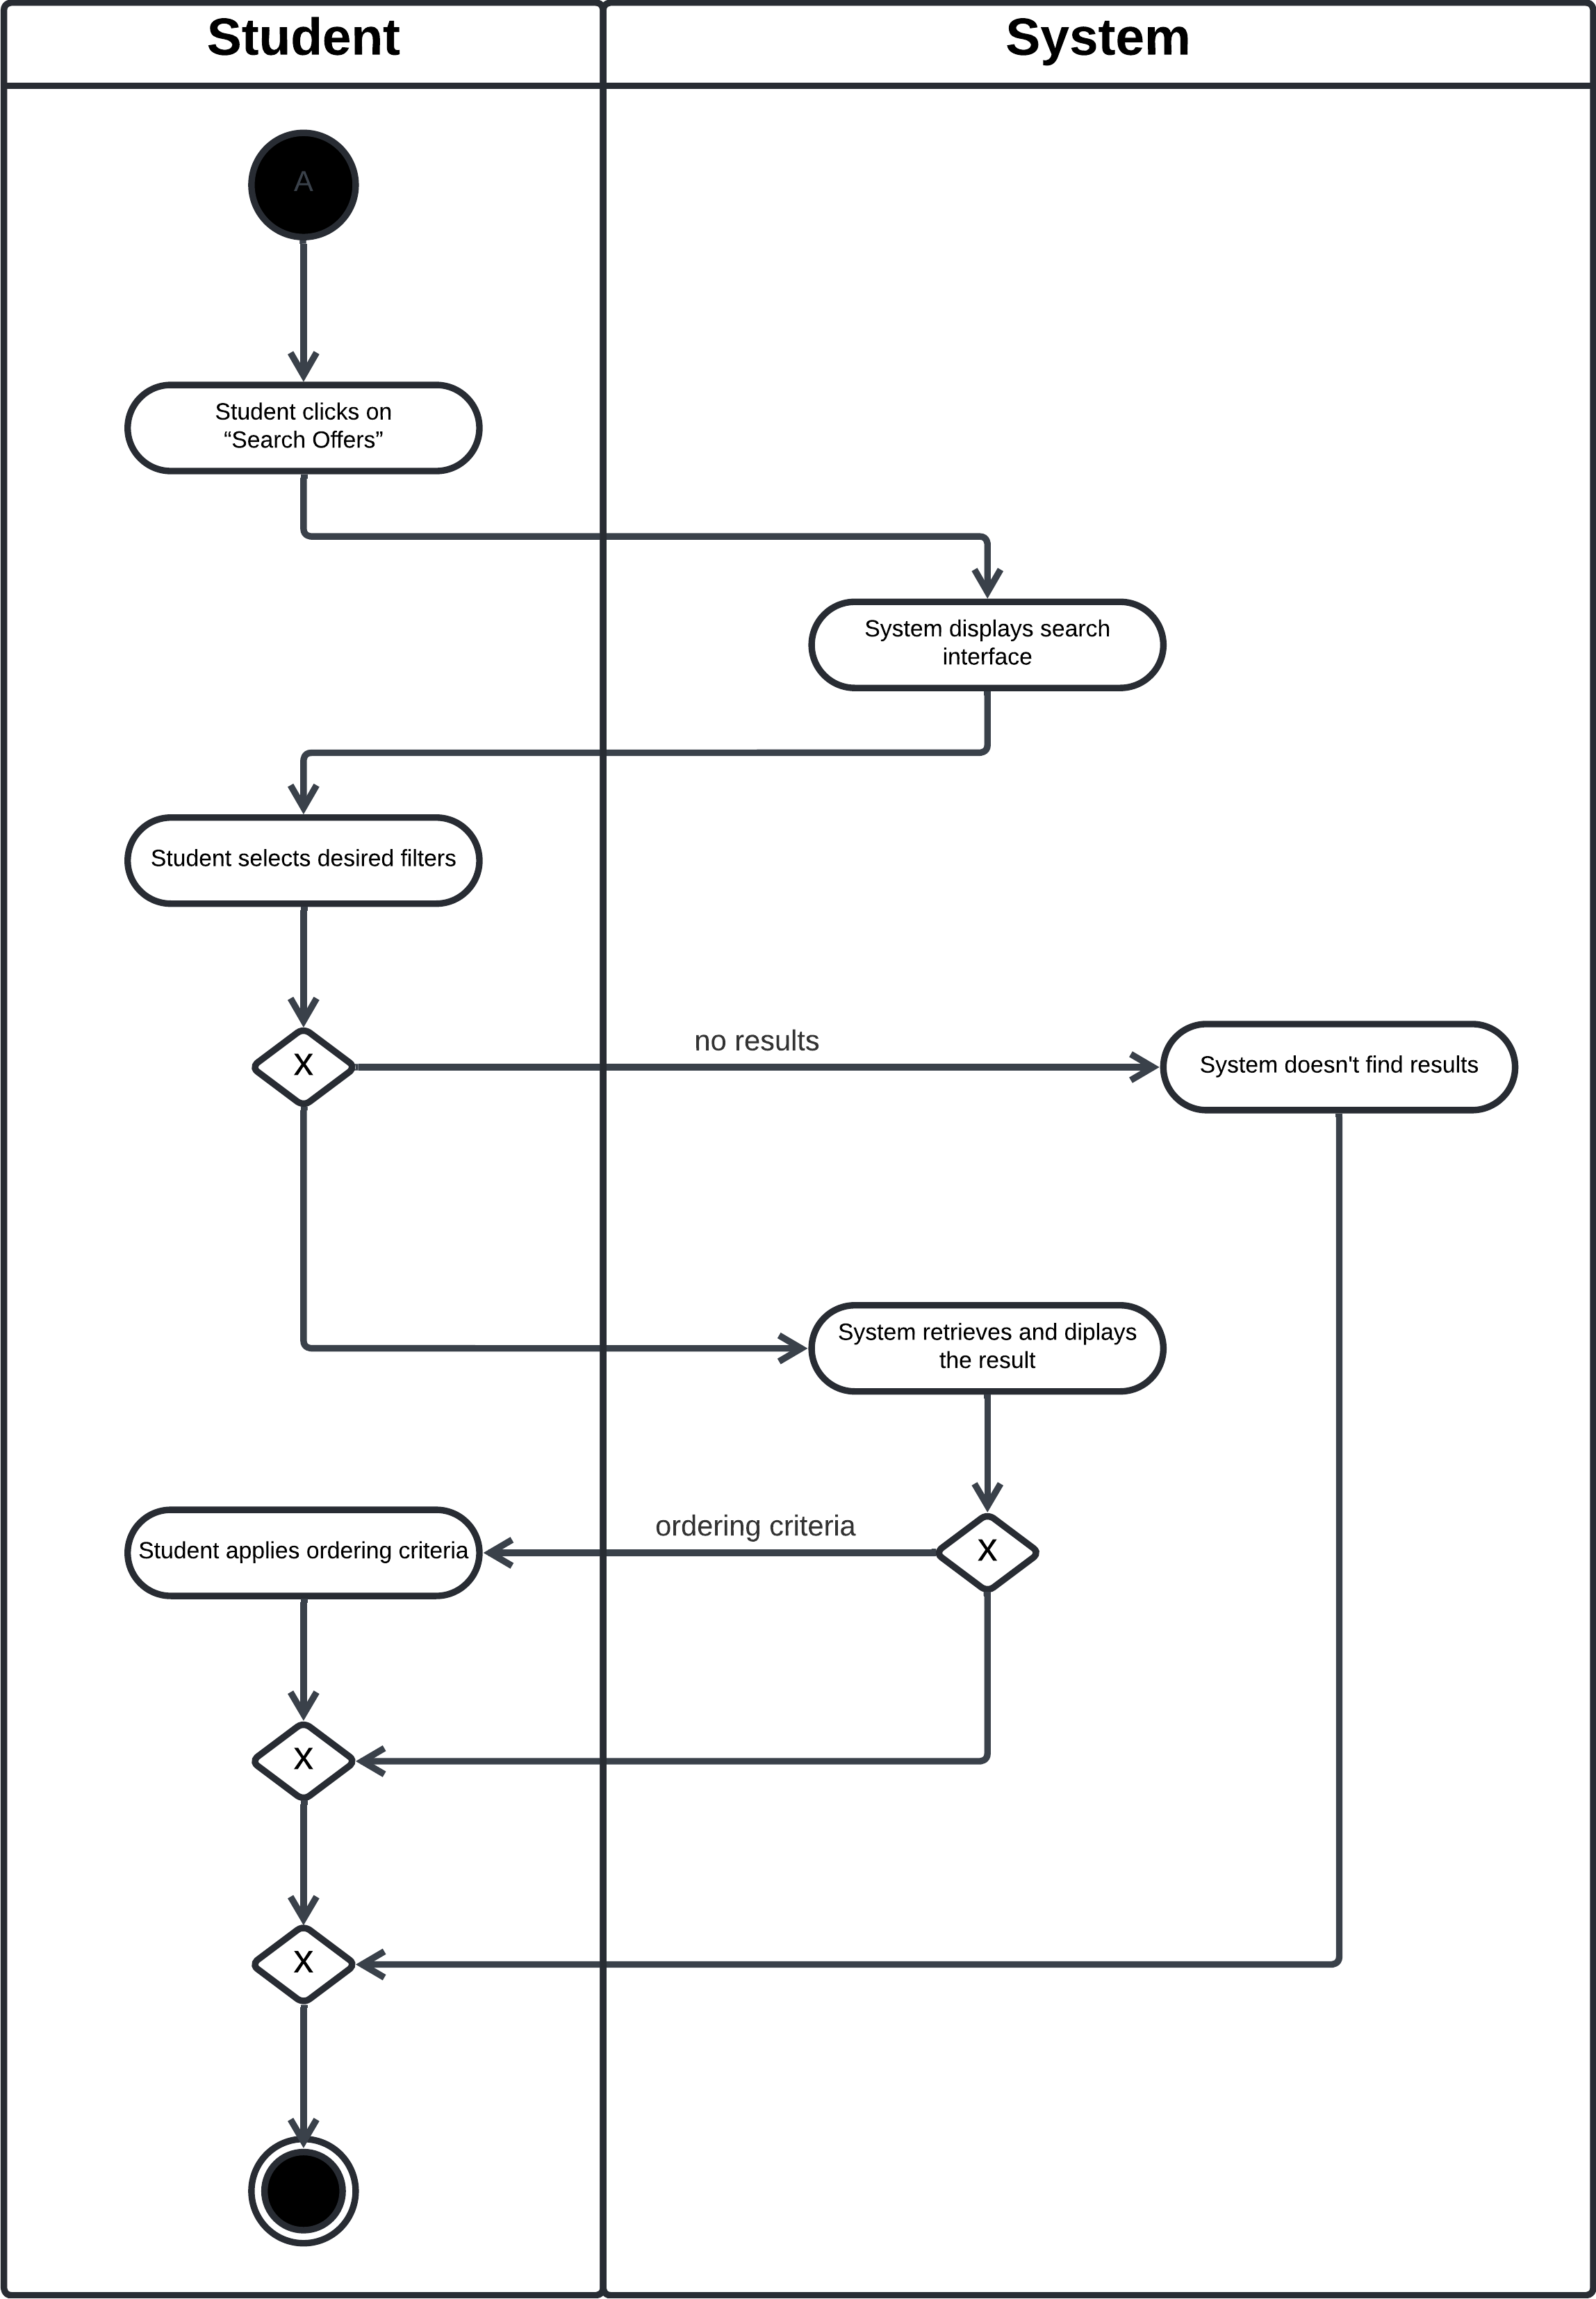
\includegraphics[width=1\linewidth]{LaTeXCode/images/activity diagram/UC8.png}
         \caption{Search Internship Offers}
         \label{fig:search_offer_ad}
     \end{center}
\end{figure}

\newpage

\subsubsection*{UC\cuc . Apply to an Internship Offer}
\begin{center}
    \begin{longtable}{|l|p{0.75\linewidth}|}
        \hline
        \textbf{Actor}            & Student \\
        \hline
        \textbf{Entry Conditions} & The Student is logged into the S\&C platform and is on the page of an internship offer. \\
        \hline
        \textbf{Flow of Events}       
        & \cucsteps. On the internship offer page, the Student clicks the "Apply" button. \\
        & \cucsteps. The system adds the application to the internship offer's candidates list. \\
        & \cucsteps. The system marks all the "Unhandled" recommendations of the Student about the selected internship offer as "Accepted" and discards all the "Unhandled" recommendations of the offering Company about them. \\
        & \cucsteps. The system confirms to the Student that the application has been successfully registered into the system. \\
        \hline
        \textbf{Exit Conditions}   & The Student has successfully made an application to an internship offer of his choice. \\
        \hline
        \textbf{Exceptions}       & \begin{itemize}
            \item The deadline for applying to the internship has expired: the "Apply" button cannot be clicked and the Student has to give up on applying.
        \end{itemize}\\
        \hline
    \end{longtable}
\end{center}
\label{subsec: apply_to_internships_uc}

\begin{figure}[H]
    \begin{center}
         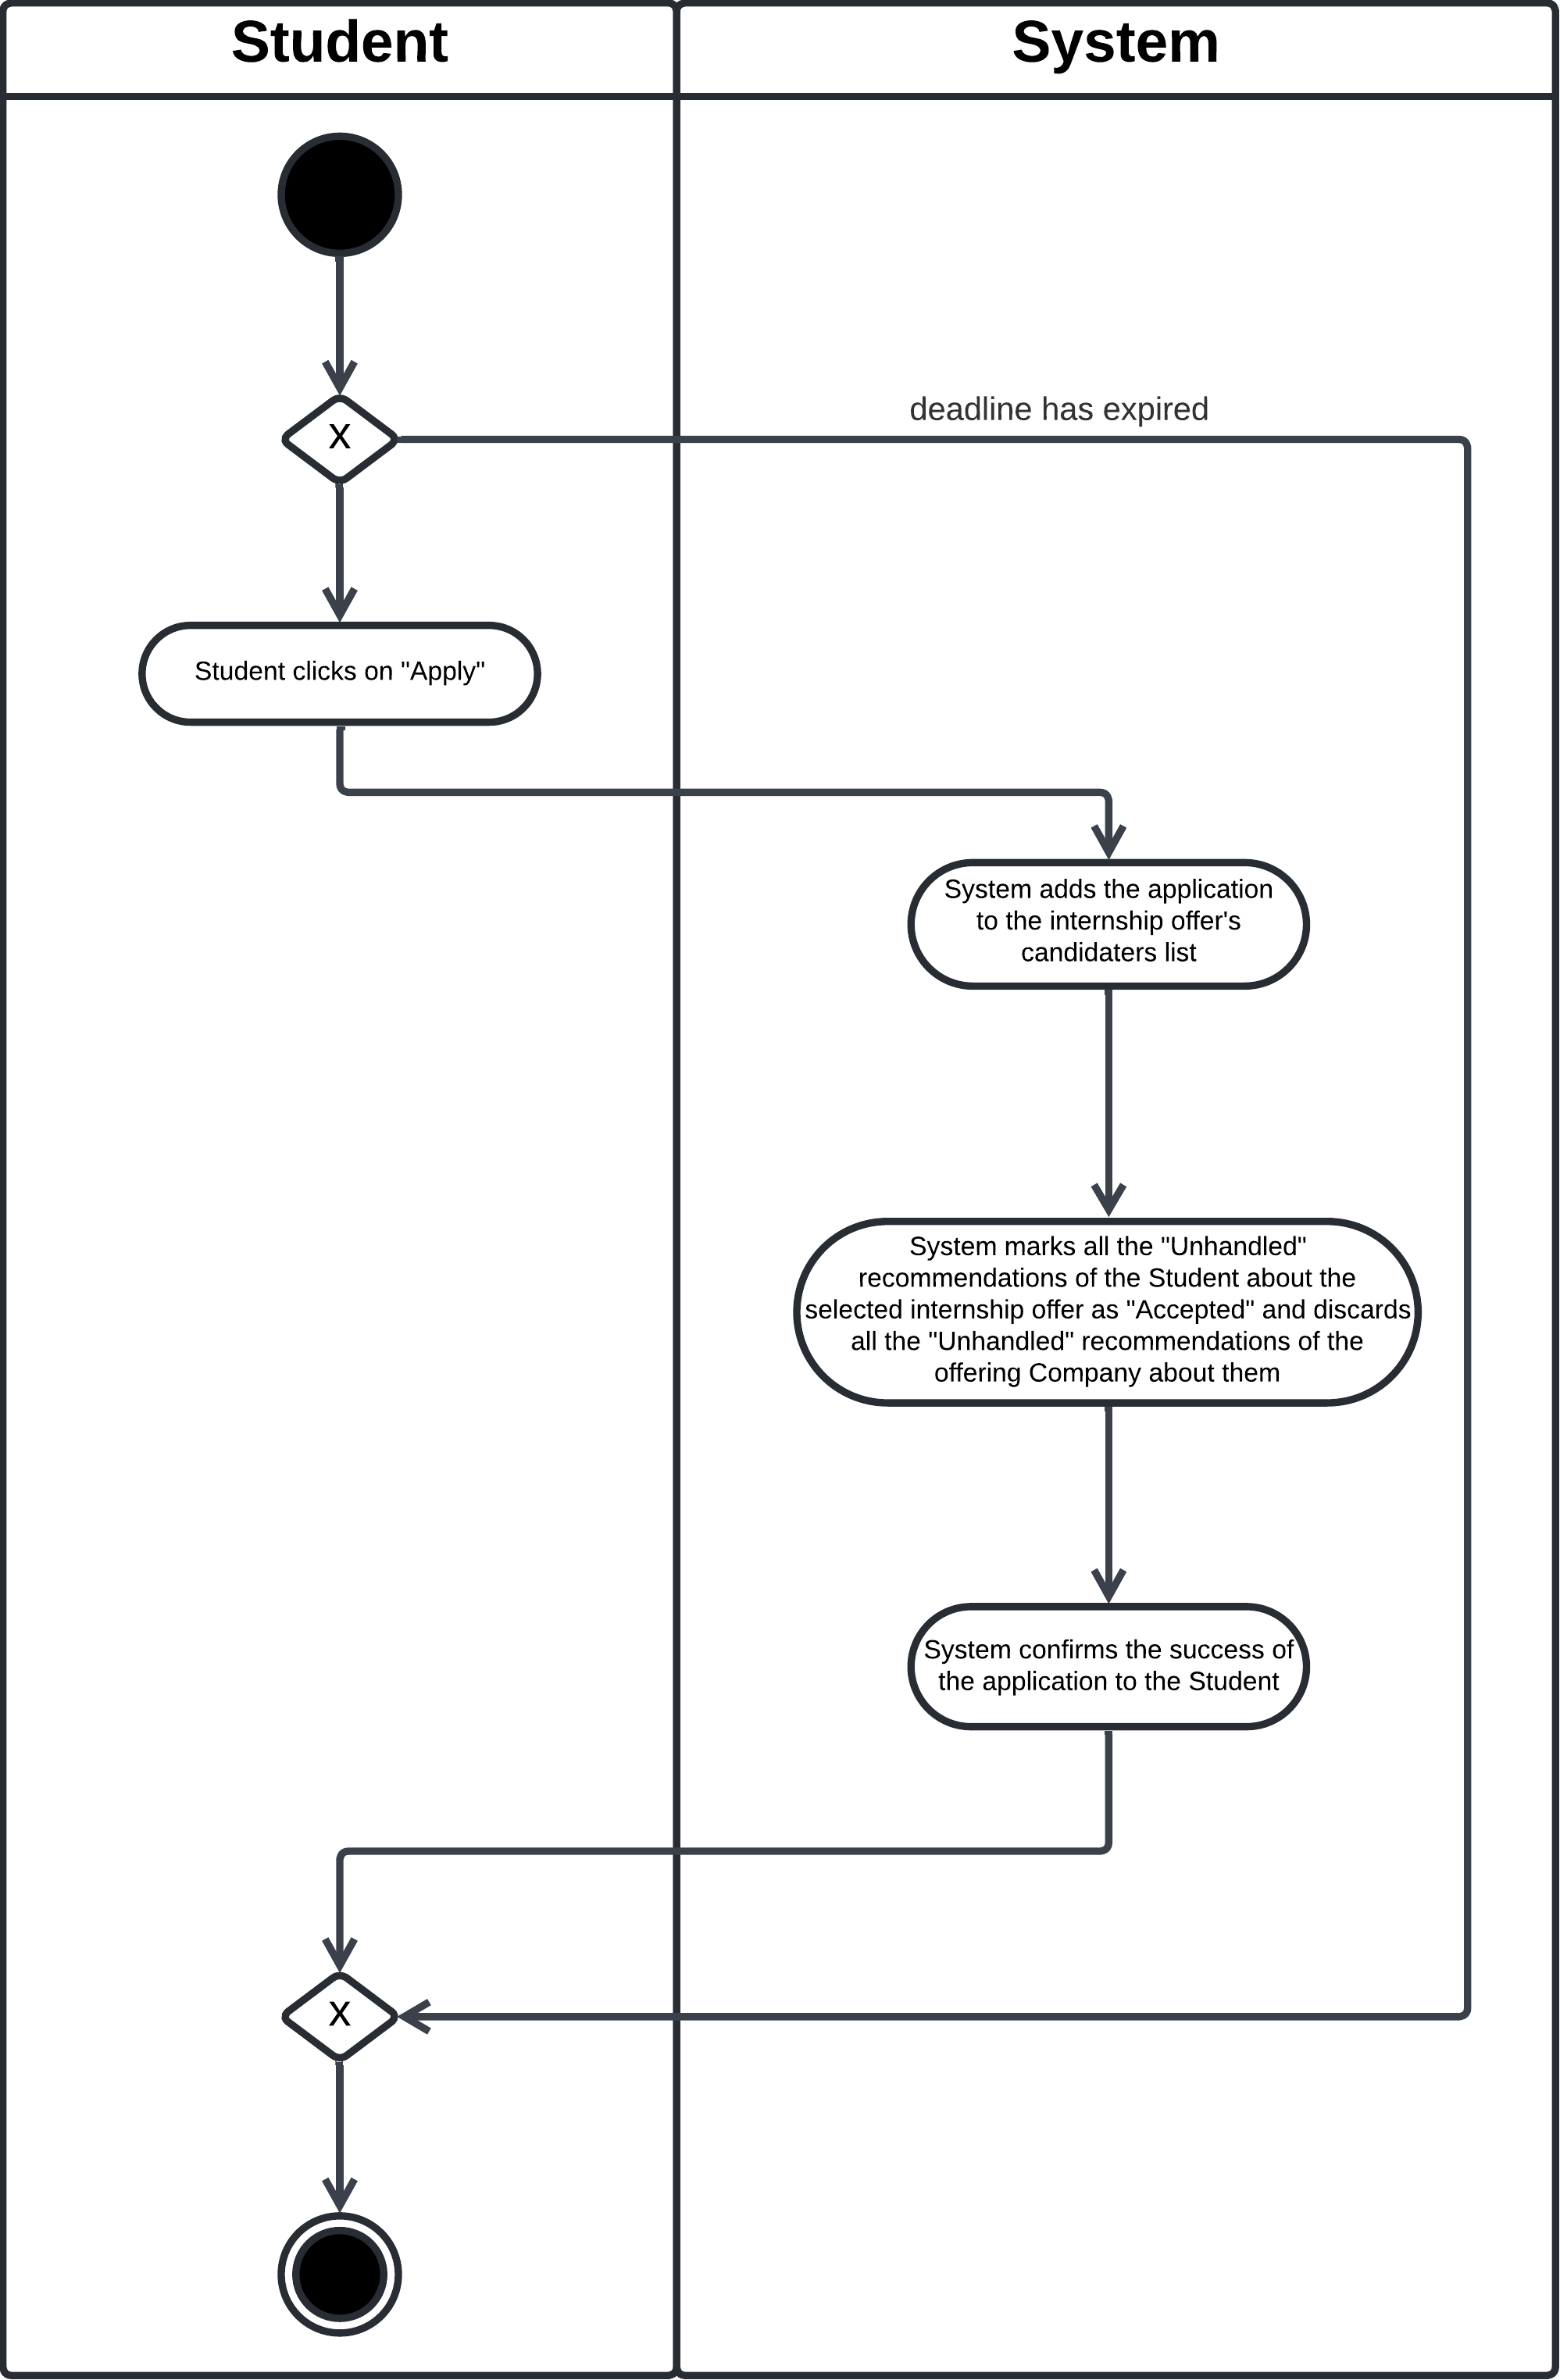
\includegraphics[width=0.9\linewidth]{LaTeXCode/images/activity diagram/UC9.png}
         \caption{Apply to an Internship Offer}
         \label{fig:apply_to_internships_ad}
     \end{center}
\end{figure}

\newpage

\subsubsection*{UC\cuc . Generate Recommendations}
\begin{center}
    \begin{longtable}{|l|p{0.75\linewidth}|}
        \hline
        \textbf{Actor}            & None\\
        \hline
        \textbf{Entry Conditions} & A relevant change in the system's information set has occurred, with the possibility of new matches between a Student and a Company emerging. \\
        \hline
        \textbf{Flow of Events}
        & \cucsteps. By taking into account the newly updated information and a subset of information from all the students, internship offers and companies, including feedback previously expressed by the parties on the platform, the system identifies every new potential match between a Student and an internship offer by a Company that has arisen as a consequence of the update of the information set and had never been identified before. In order to be considered, a match that had already been identified previously and subsequently discarded by a Party needs to have been generated by a substantial change in the information set (with the threshold possibly increasing). \\ 
        & \cucsteps. For every new match, the system generates a recommendation for the identified Parties, which could be only the Student, only the Company or both. Then, the system adds it to the list of recommendations of such Parties. \\
        \hline
        \textbf{Exit Condition}   & The generated recommendations have been posted on the respective Parties' dashboards. \\       
        \hline
        \textbf{Exceptions}       & \begin{itemize}
            \item The system doesn't find any match: it terminates the process silently. 
        \end{itemize}\\
        \hline
    \end{longtable}
\end{center}
\label{subsec: generate_recommendations_uc}

\begin{figure}[H]
    \begin{center}
         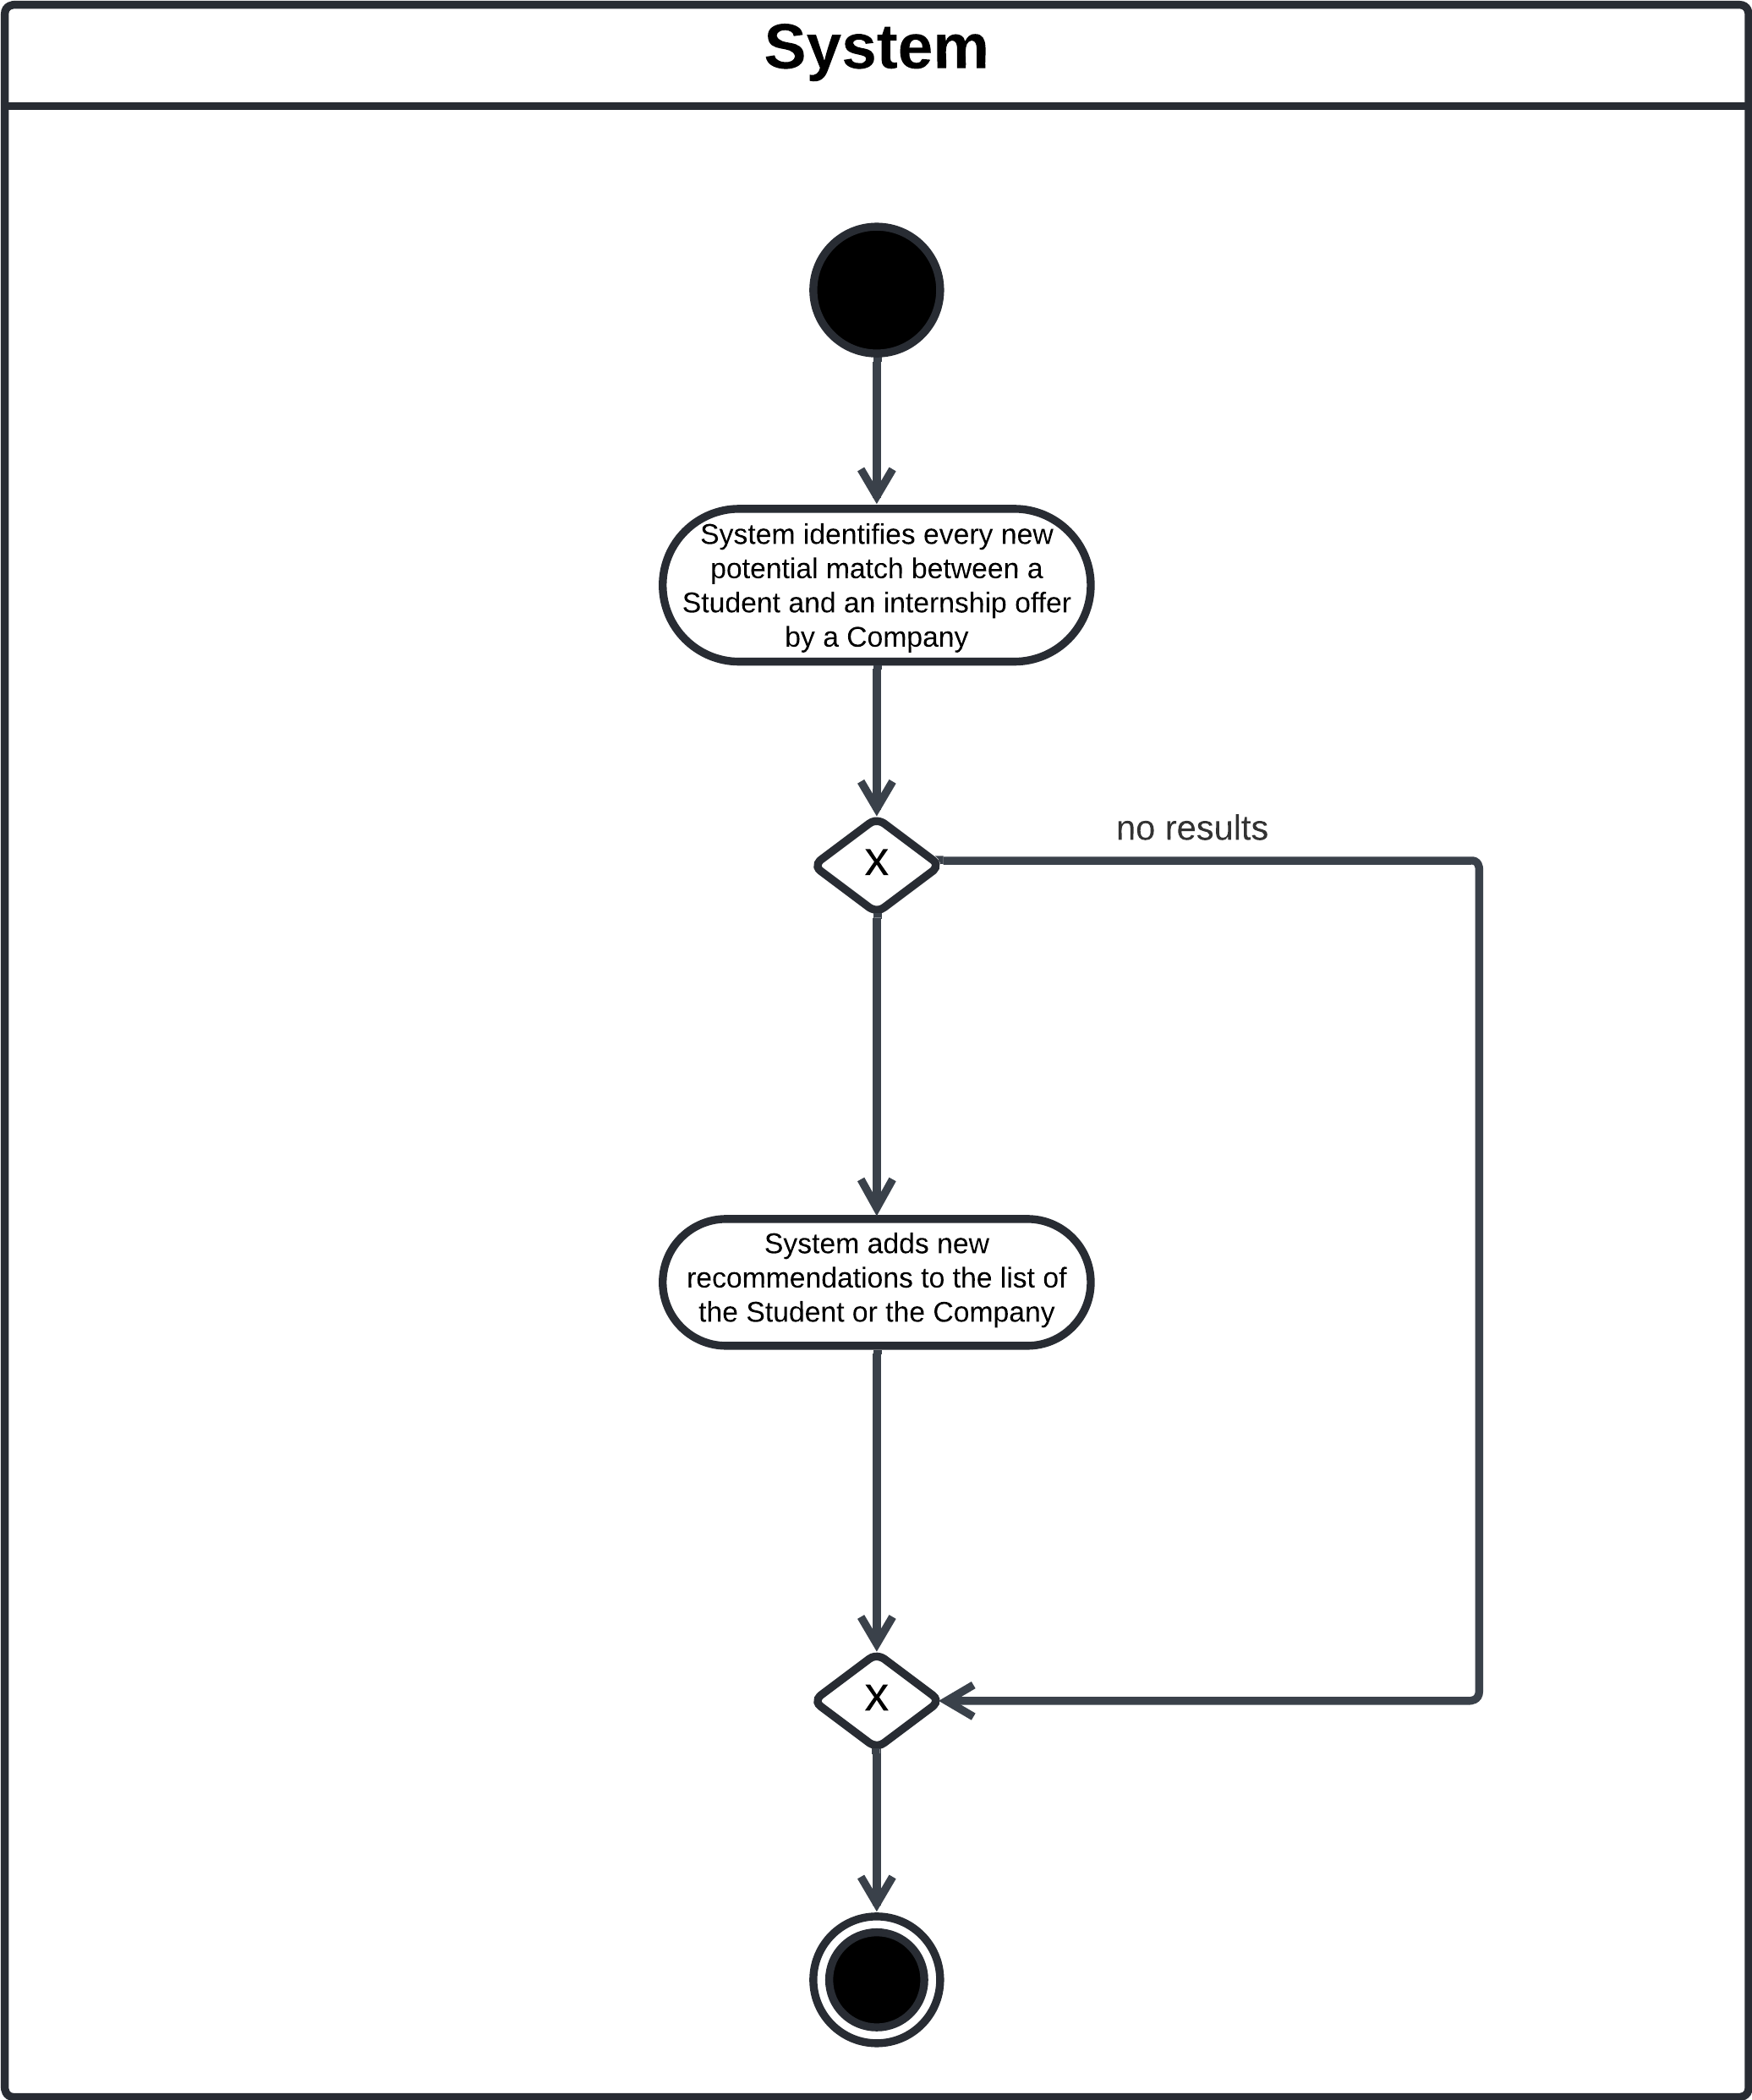
\includegraphics[width=0.9\linewidth]{LaTeXCode/images/activity diagram/UC10.png}
         \caption{Generate Recommendations}
         \label{fig:generate_recommendations_ad}
     \end{center}
\end{figure}

\newpage

\subsubsection*{UC\cuc . Manage Internship Recommendations}
\begin{center}
    \begin{longtable}{|l|p{0.75\linewidth}|}
        \hline
        \textbf{Actor}            & Student \\
        \hline
        \textbf{Entry Conditions} & The Student is logged in and has received at least one recommendation about an internship offer. \\
        \hline
        \textbf{Flow of Events} 
        & \cucsteps. In the dashboard, the Student navigates to the "Manage Recommendations" section. \\
        & \cucsteps. The system displays a list of recommended internship offers for the Student, along with their and the offering Company's information. \\
        & \cucsteps. The Student reviews the list of recommended internship offers, evaluating them. \\
        & \cucsteps. The Student selects a specific recommendation, which expands showing the internship offer details. \\
        & \theucsteps. The student can perform one of the following actions: accept, reject, or postpone the decision. \\
        & \theucsteps.1. If the Student accepts the recommendation, the system automatically performs an "Apply" operation via the \hyperref[subsec: apply_to_internships_uc]{\uline{UC. Apply to an Internship Offer}} to the corresponding internship offer; the system also removes the recommendation from visualization. \\
        & \theucsteps.2. If the Student rejects the recommendation, the latter is simply removed from visualization by the system. \\
        & \cucsteps.3. If the Student chooses to postpone the decision, the system doesn't perform any operation.\\
        & \cucsteps. The Student may repeat this process until there are no pending recommendations.\\
        \hline
        \textbf{Exit Conditions}   & The decision on the selected recommendations is recorded, and the internship offers' statuses are updated accordingly in the system. \\
        \hline
        \textbf{Exceptions}       & None \\
        \hline
    \end{longtable}
\end{center}

\begin{figure}[H]
    \begin{center}
         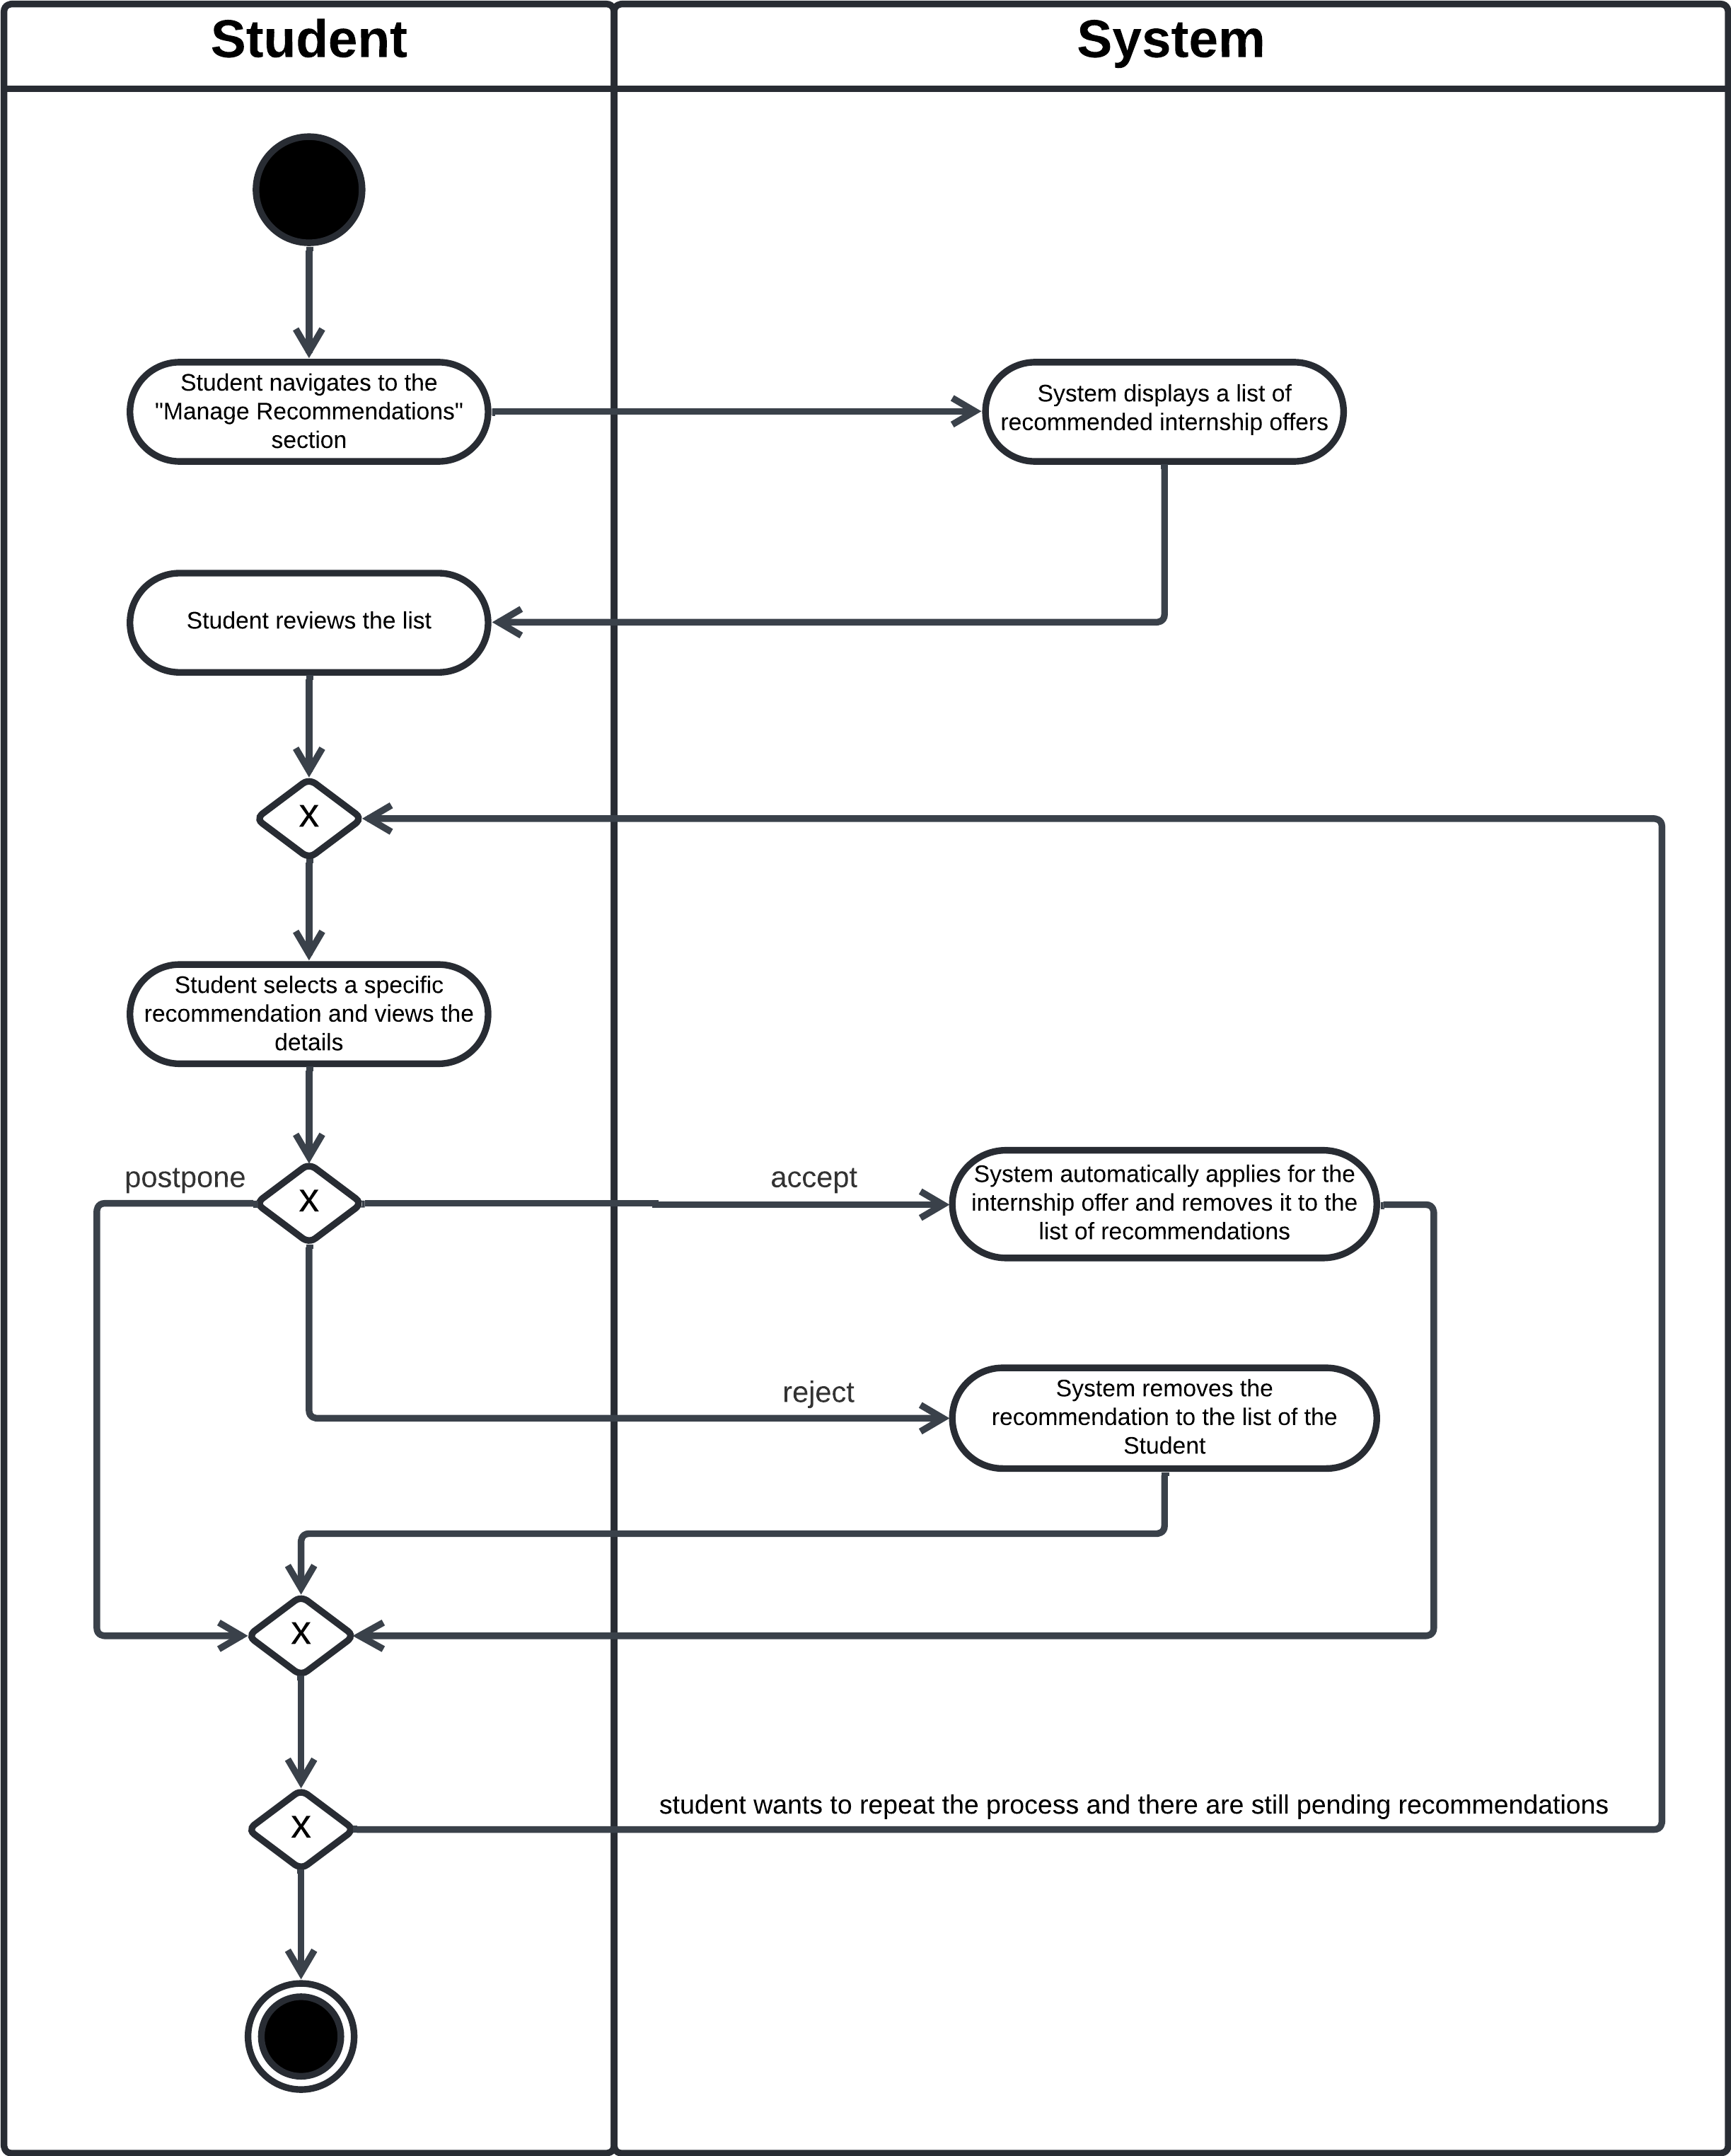
\includegraphics[width=1\linewidth]{LaTeXCode/images/activity diagram/UC11.png}
         \caption{Manage Internship Recommendations}
         \label{fig:manage_internship_recommendations_ad}
     \end{center}
\end{figure}

\newpage

\subsubsection*{UC\cuc . Manage Students Recommendations}
\begin{center}
    \begin{longtable}{|l|p{0.75\linewidth}|}
        \hline
        \textbf{Actor}            & Company \\
        \hline
        \textbf{Entry Conditions} & The Company is logged in and has received at least one recommendation about a Student for any of their internship offers. \\
        \hline
        \textbf{Flow of Events} 
        & \cucsteps. In the dashboard, the Company navigates to the "Manage Recommendations" section. \\
        & \cucsteps. The system displays a list of recommended students for the available internship offers, along with their profile information. \\
        & \cucsteps. The Company reviews the list of recommended students, evaluating them. \\
        & \cucsteps. The Company selects a specific recommendation, which expands showing the student's profile. \\
        & \theucsteps. The Company can perform one of the following actions: accept, reject, or postpone the decision.\\
        & \theucsteps.1. If the Company accepts the recommendation, the system marks it as "Selected" and the corresponding Student receives a dual recommendation, on which they will be able to decide; the system also removes the recommendation from visualization. \\
        & \theucsteps.2. If the Company rejects the recommendation, the latter is simply removed from visualization by the system. \\
        & \cucsteps.3. If the Company chooses to postpone the decision, the system doesn't perform any operation.\\
        & \cucsteps. The Company may repeat this process until there are no pending recommendations.\\
        \hline
        \textbf{Exit Conditions}   & The decision on the selected recommendations is recorded, and the students' statuses are updated accordingly in the system. \\
        \hline
        \textbf{Exceptions}       & None \\
        \hline
    \end{longtable}
\end{center}

\begin{figure}[H]
    \begin{center}
         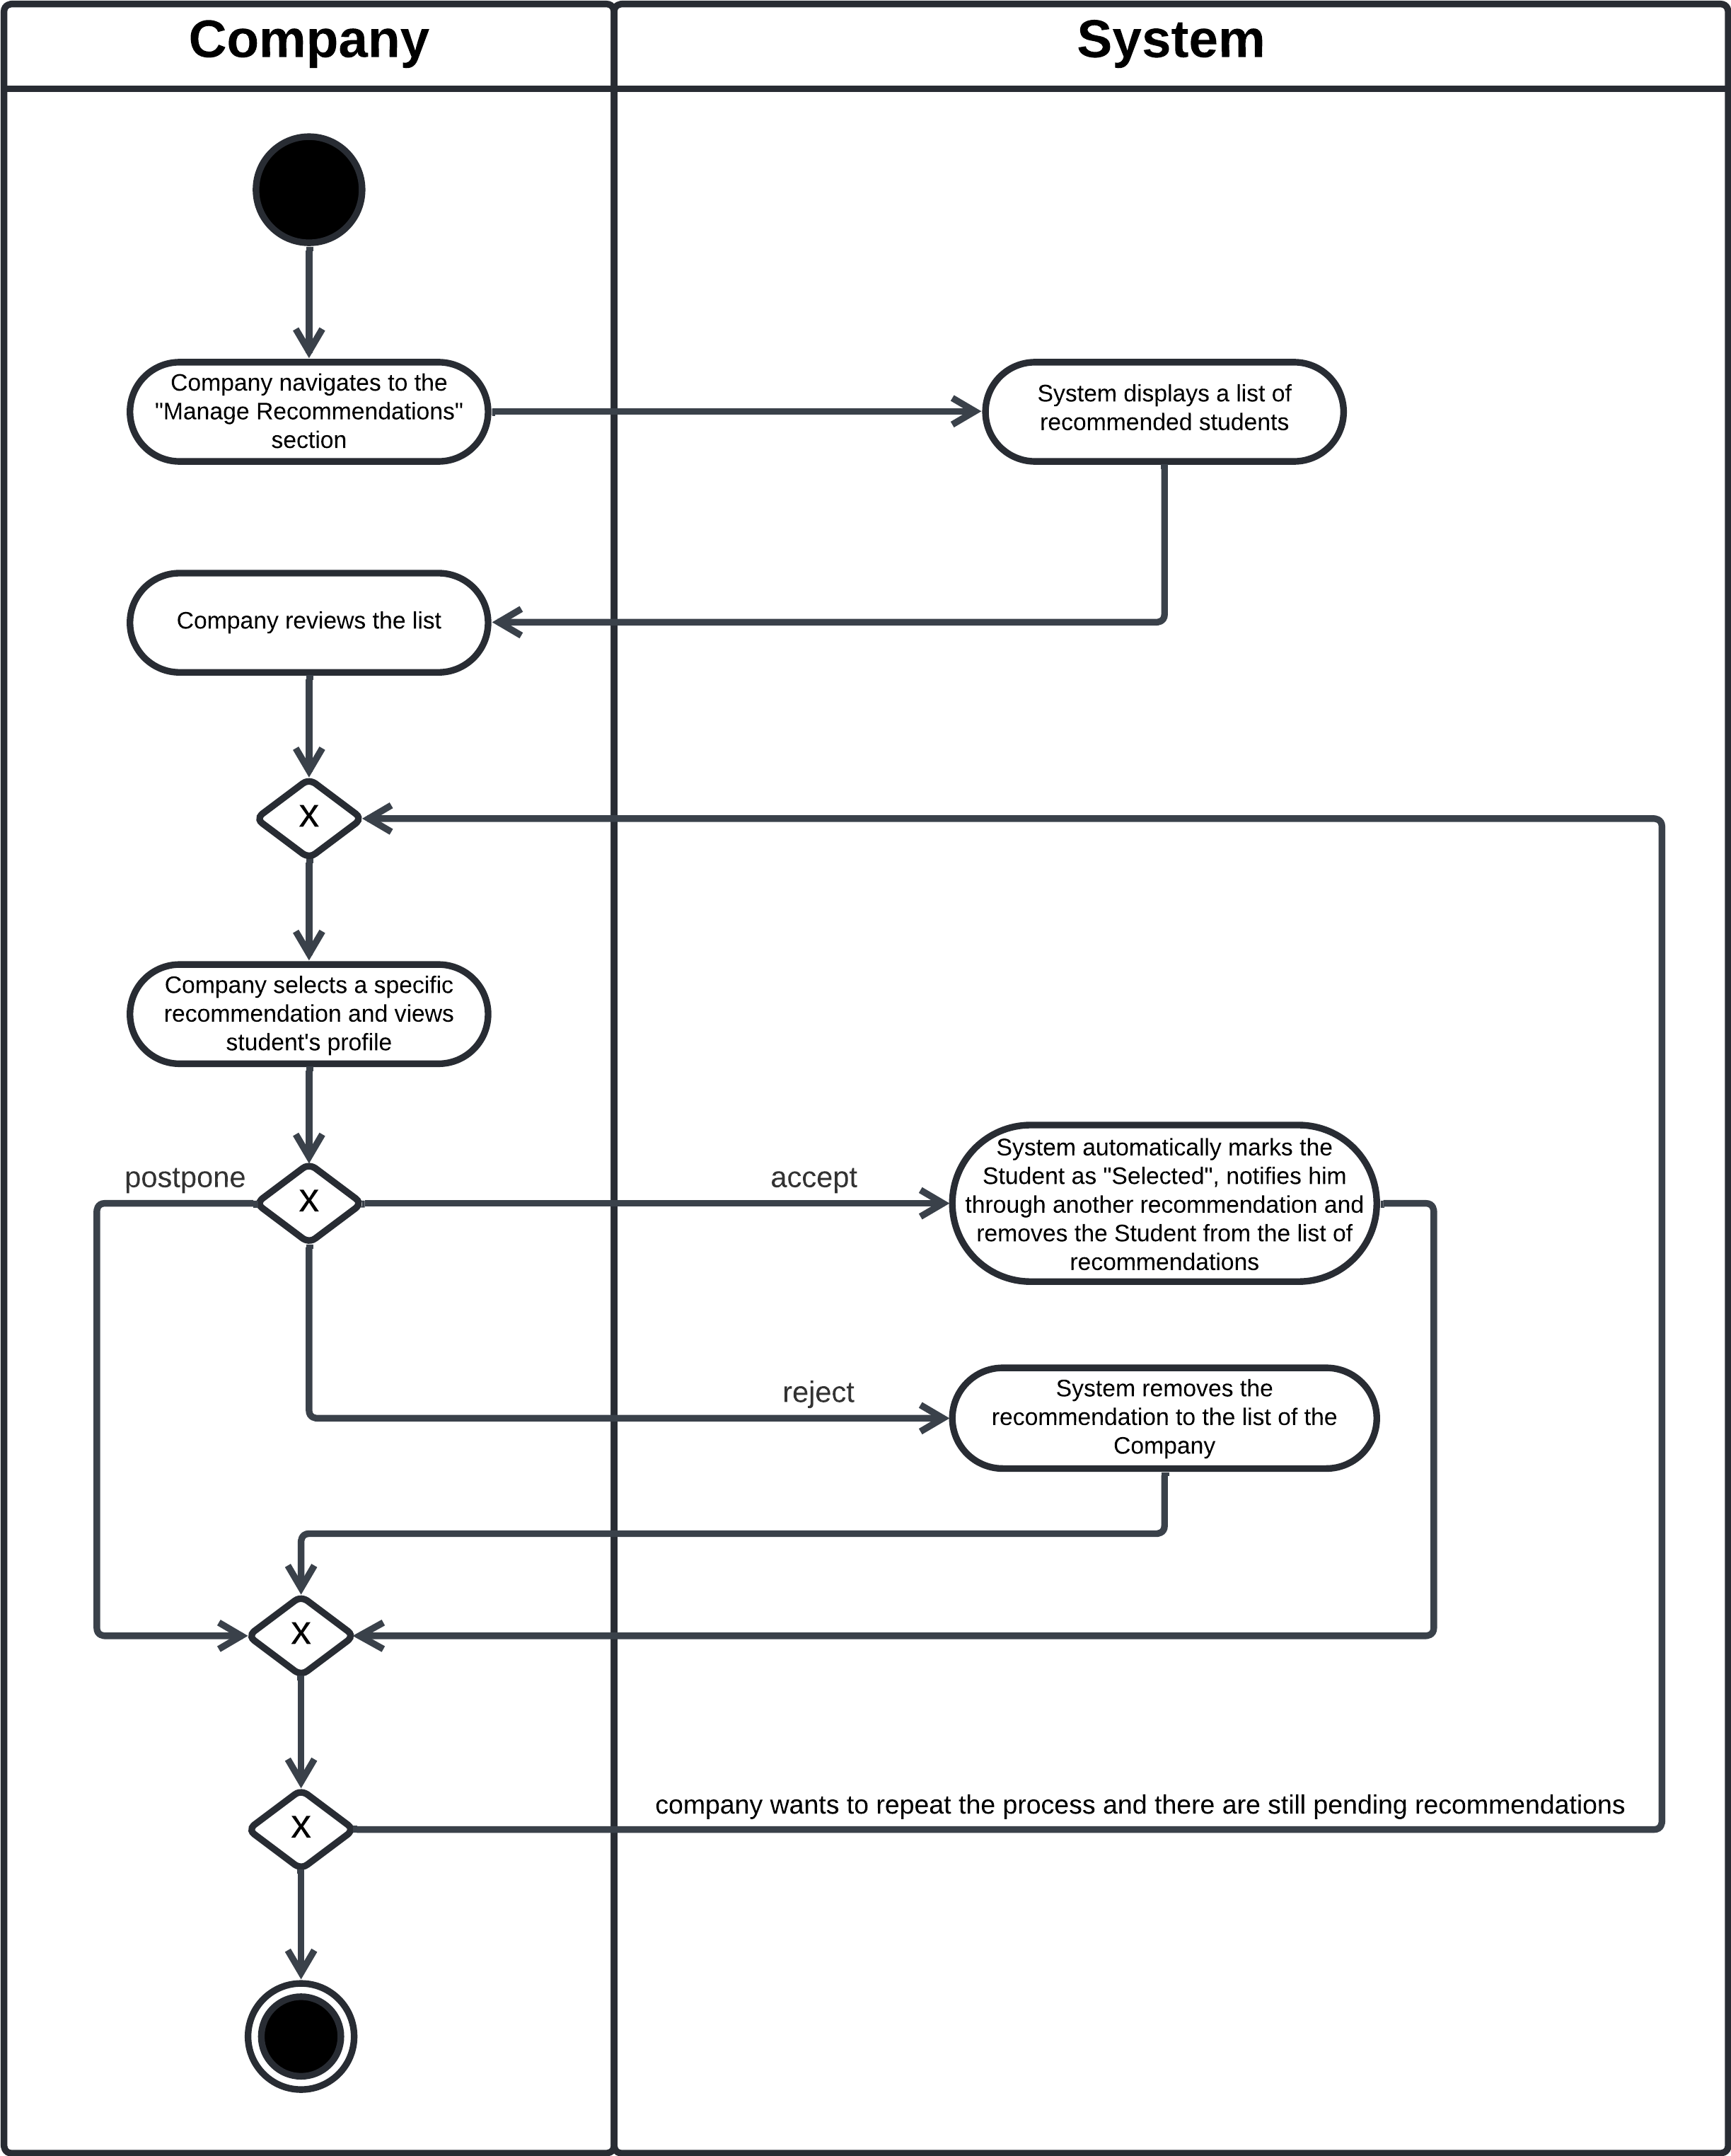
\includegraphics[width=1\linewidth]{LaTeXCode/images/activity diagram/UC12.png}
         \caption{Manage Students Recommendations}
         \label{fig:manage_students_recommendations_ad}
     \end{center}
\end{figure}

\newpage

\subsubsection*{UC\cuc . Manage an Interview}
\begin{center}
    \begin{longtable}{|l|p{0.75\linewidth}|}
        \hline
        \textbf{Actor}            & Company, Student\\
        \hline
        \textbf{Entry Conditions} & The application deadline for a specific internship offer has expired and the Company has accepted at least one application to that offer, establishing a contact with the accepted Student.\\
        \hline
        \textbf{Flow of Events}       
        & \cucsteps. From the dashboard page, the Company navigates to the page of one of its internship offers.\\
        & \cucsteps. On the internship offer page, the Company selects a Student from the list of candidates for that offer, opening a new page to arrange the interview. \\ 
        & \cucsteps. The Company creates an interview invitation to the Student, specifying the date, time, format (in-platform or in-person) and an optional text description with more details. \\
        & \cucsteps. The Company reviews and forwards the interview invitation by confirming its information through the "Confirm" button. \\
        & \cucsteps. The Student receives the invitation to the interview on the corresponding section of its dashboard page and navigates to the platform to review the invitation details. \\
        & \theucsteps. The Student accepts or declines the interview invitation, confirming their preference. If declining, he is able to provide a reason behind the choice, so that the Company may reschedule the interview.\\
        & \theucsteps.1. If the Student accepts the invitation, the interview is conducted according to the specified details, enabling the Company to assess the student's suitability for the internship either by sharing multiple questions through the platform or by interviewing the candidate in person and later recording the results on the system.\\
        & \cucsteps.2. If the Student declines the invitation, the system marks the interview as declined. The Company sees the rejection and can decide whether to reschedule based on the given reason. \\
        & \cucsteps. After the interview, the Company provides an evaluation of the student’s performance, inserting strengths, weaknesses, and suitability for the role, and submits the results through the platform.\\
        & \cucsteps. The system records the evaluation and updates the student’s status in the selection process: "Interview Completed", "Selected" or "Rejected". \\
        \hline
        \textbf{Exit Conditions}   & The interview is completed, and the Student’s status in the selection process is updated in the system, becoming available for consulting. \\       
        \hline
        \textbf{Exceptions}       & None \\
        \hline
    \end{longtable}
\end{center}

\begin{figure}[H]
    \begin{center}
         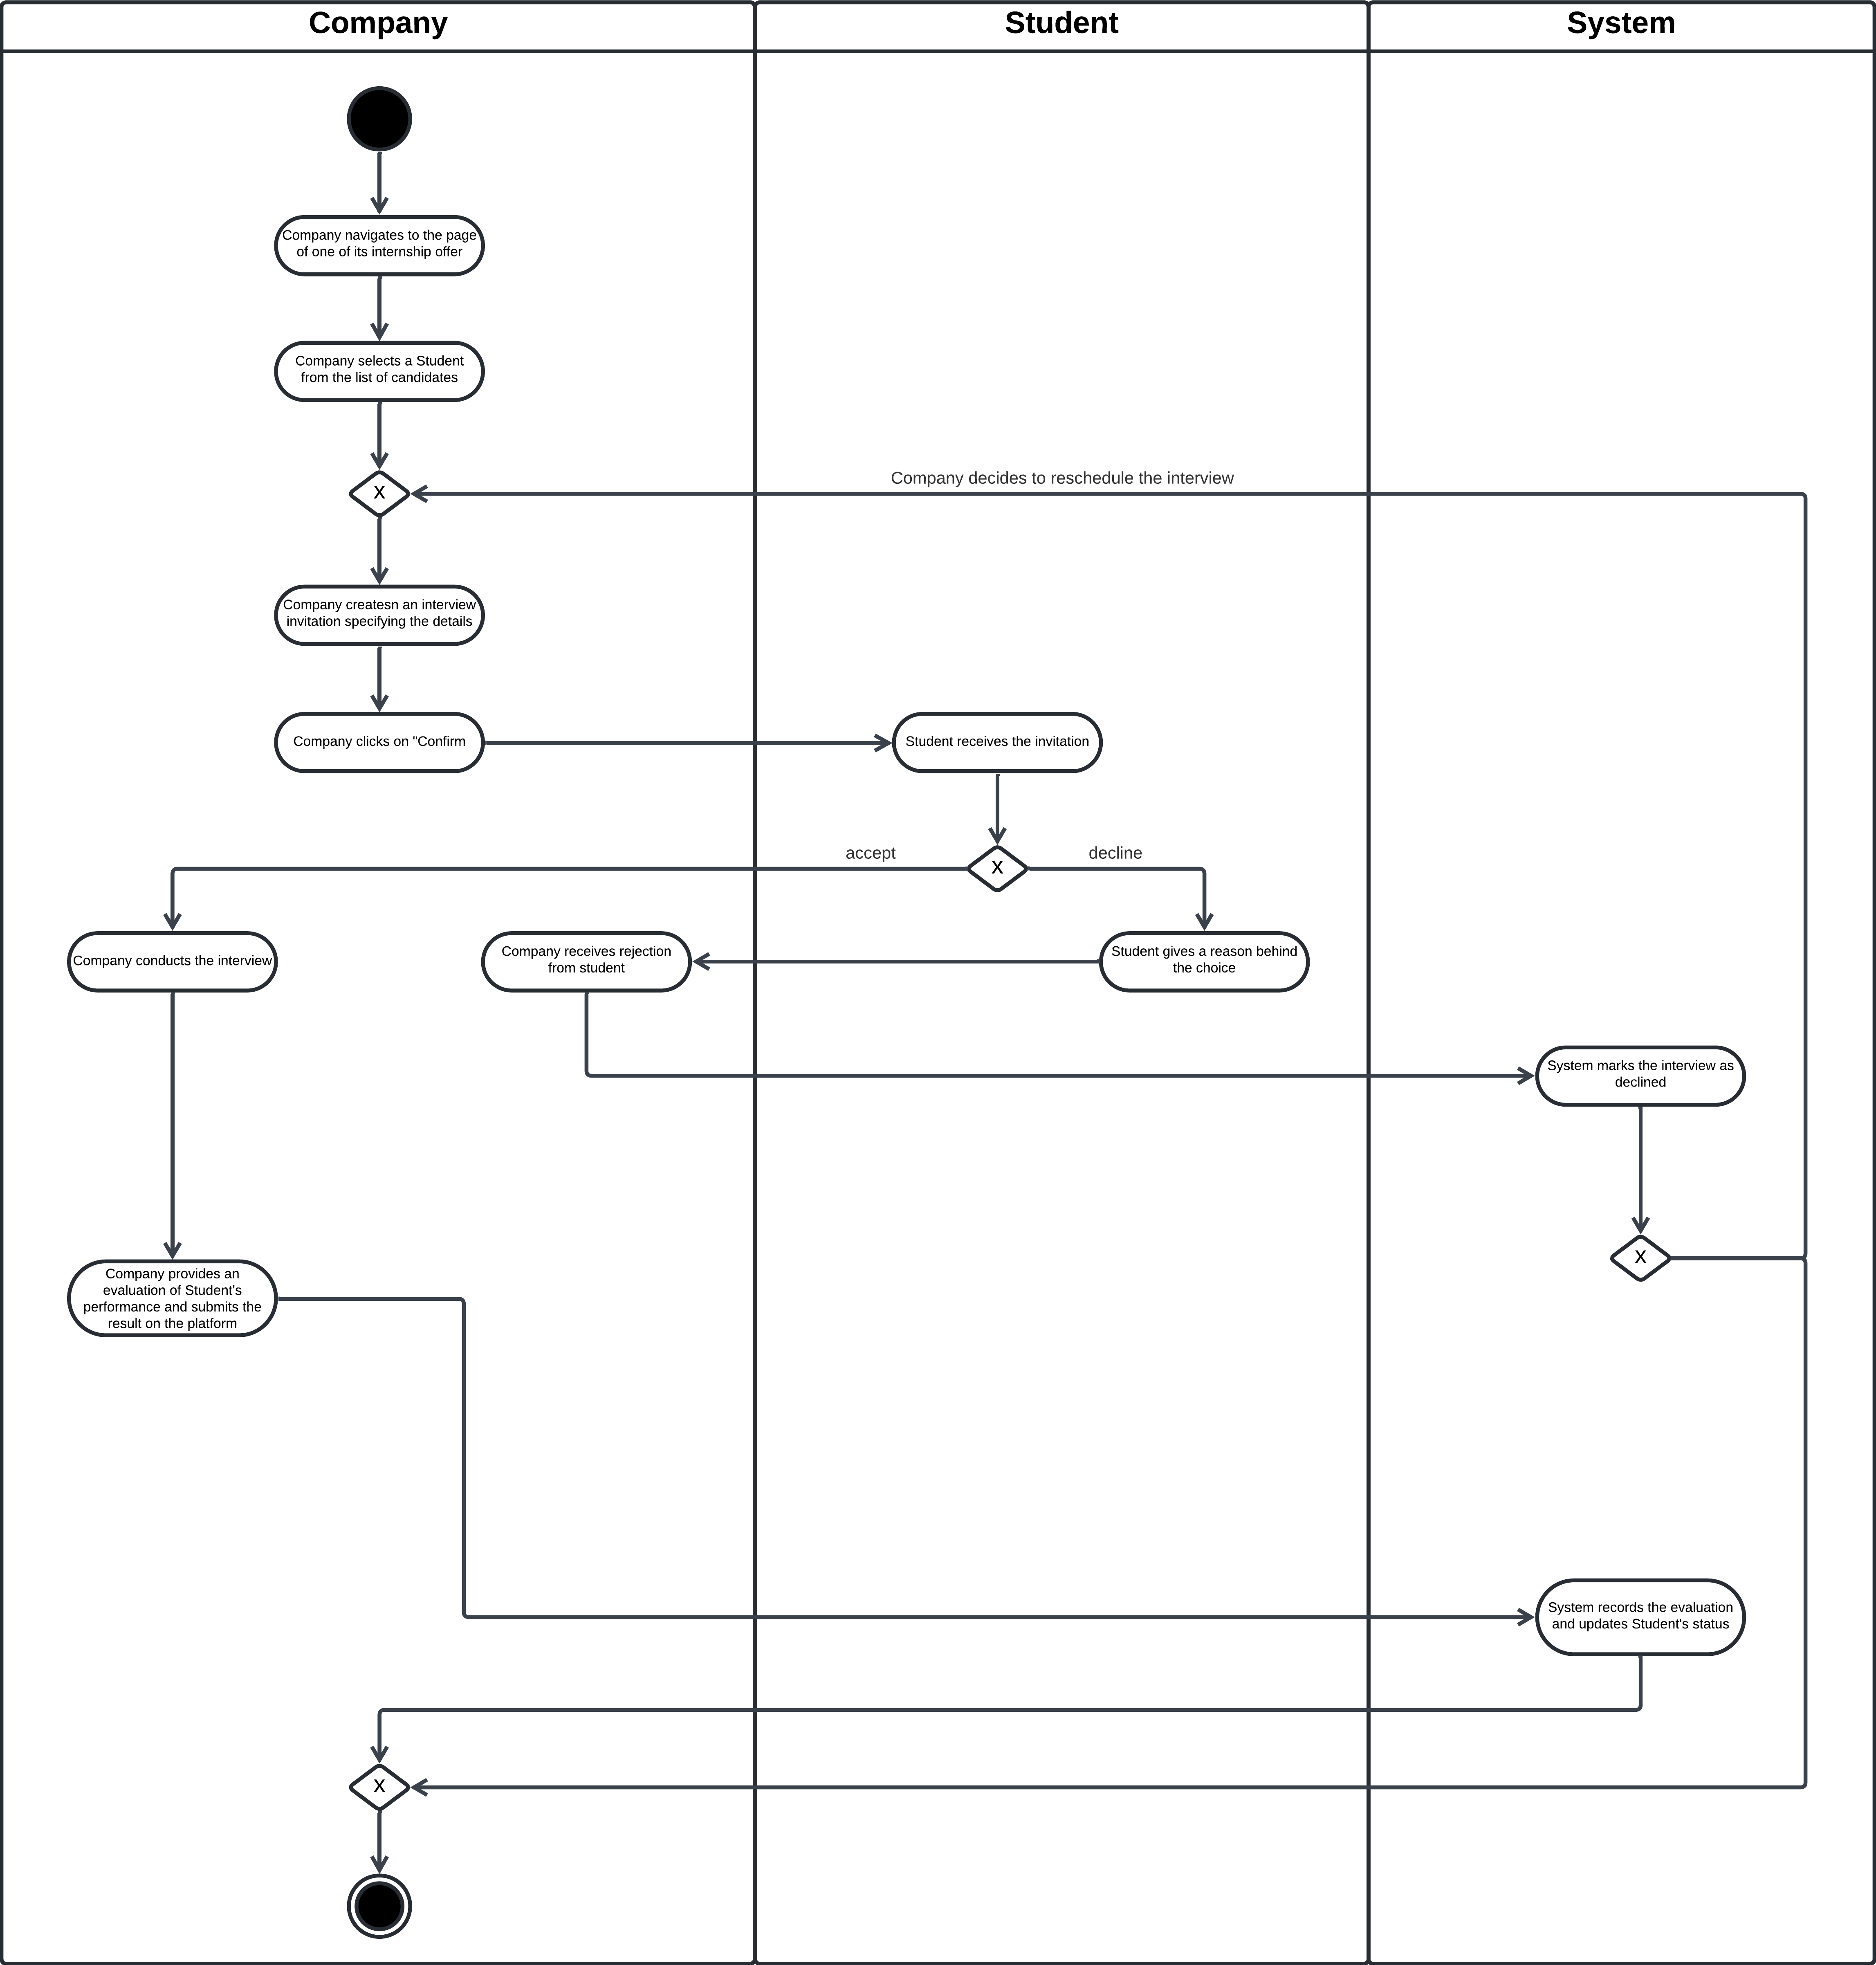
\includegraphics[width=1\linewidth]{LaTeXCode/images/activity diagram/UC13.png}
         \caption{Manage an Interview}
         \label{fig:manage_interview_ad}
     \end{center}
\end{figure}

\newpage

\subsubsection*{UC\cuc . Provide Information for an ongoing Internship}
\begin{center}
    \begin{longtable}{|l|p{0.75\linewidth}|}
        \hline
        \textbf{Actor}            & Party (Student or Company)\\
        \hline
        \textbf{Entry Conditions} & The Party is logged into the S\&C platform, is actively involved in the selected ongoing internship and has identified new information about it to be provided.\\
        \hline
        \textbf{Flow of Events}   
        & \cucsteps. On the ongoing internship's page, the Party clicks the "Post information" button. \\ 
        & \cucsteps. The Party provides new information about the selected ongoing internship in the given text field. \\
        & \cucsteps. The Party confirms the information provided by clicking the confirmation button. \\
        & \cucsteps. The system records the new information inserted and posts it on the ongoing internship's page. \\
        \hline
        \textbf{Exit Conditions}   & The ongoing internship's page is updated and those changes are recorded in the system. \\    
        \hline
        \textbf{Exceptions}       & \begin{itemize}
            \item The Party closes the page without completing the process: the system doesn't record any information and displays the Party's dashboard.
        \end{itemize} \\
        \hline 
    \end{longtable}
\end{center}
\label{subsec: provide_information_ongoing_uc}

\begin{figure}[H]
    \begin{center}
         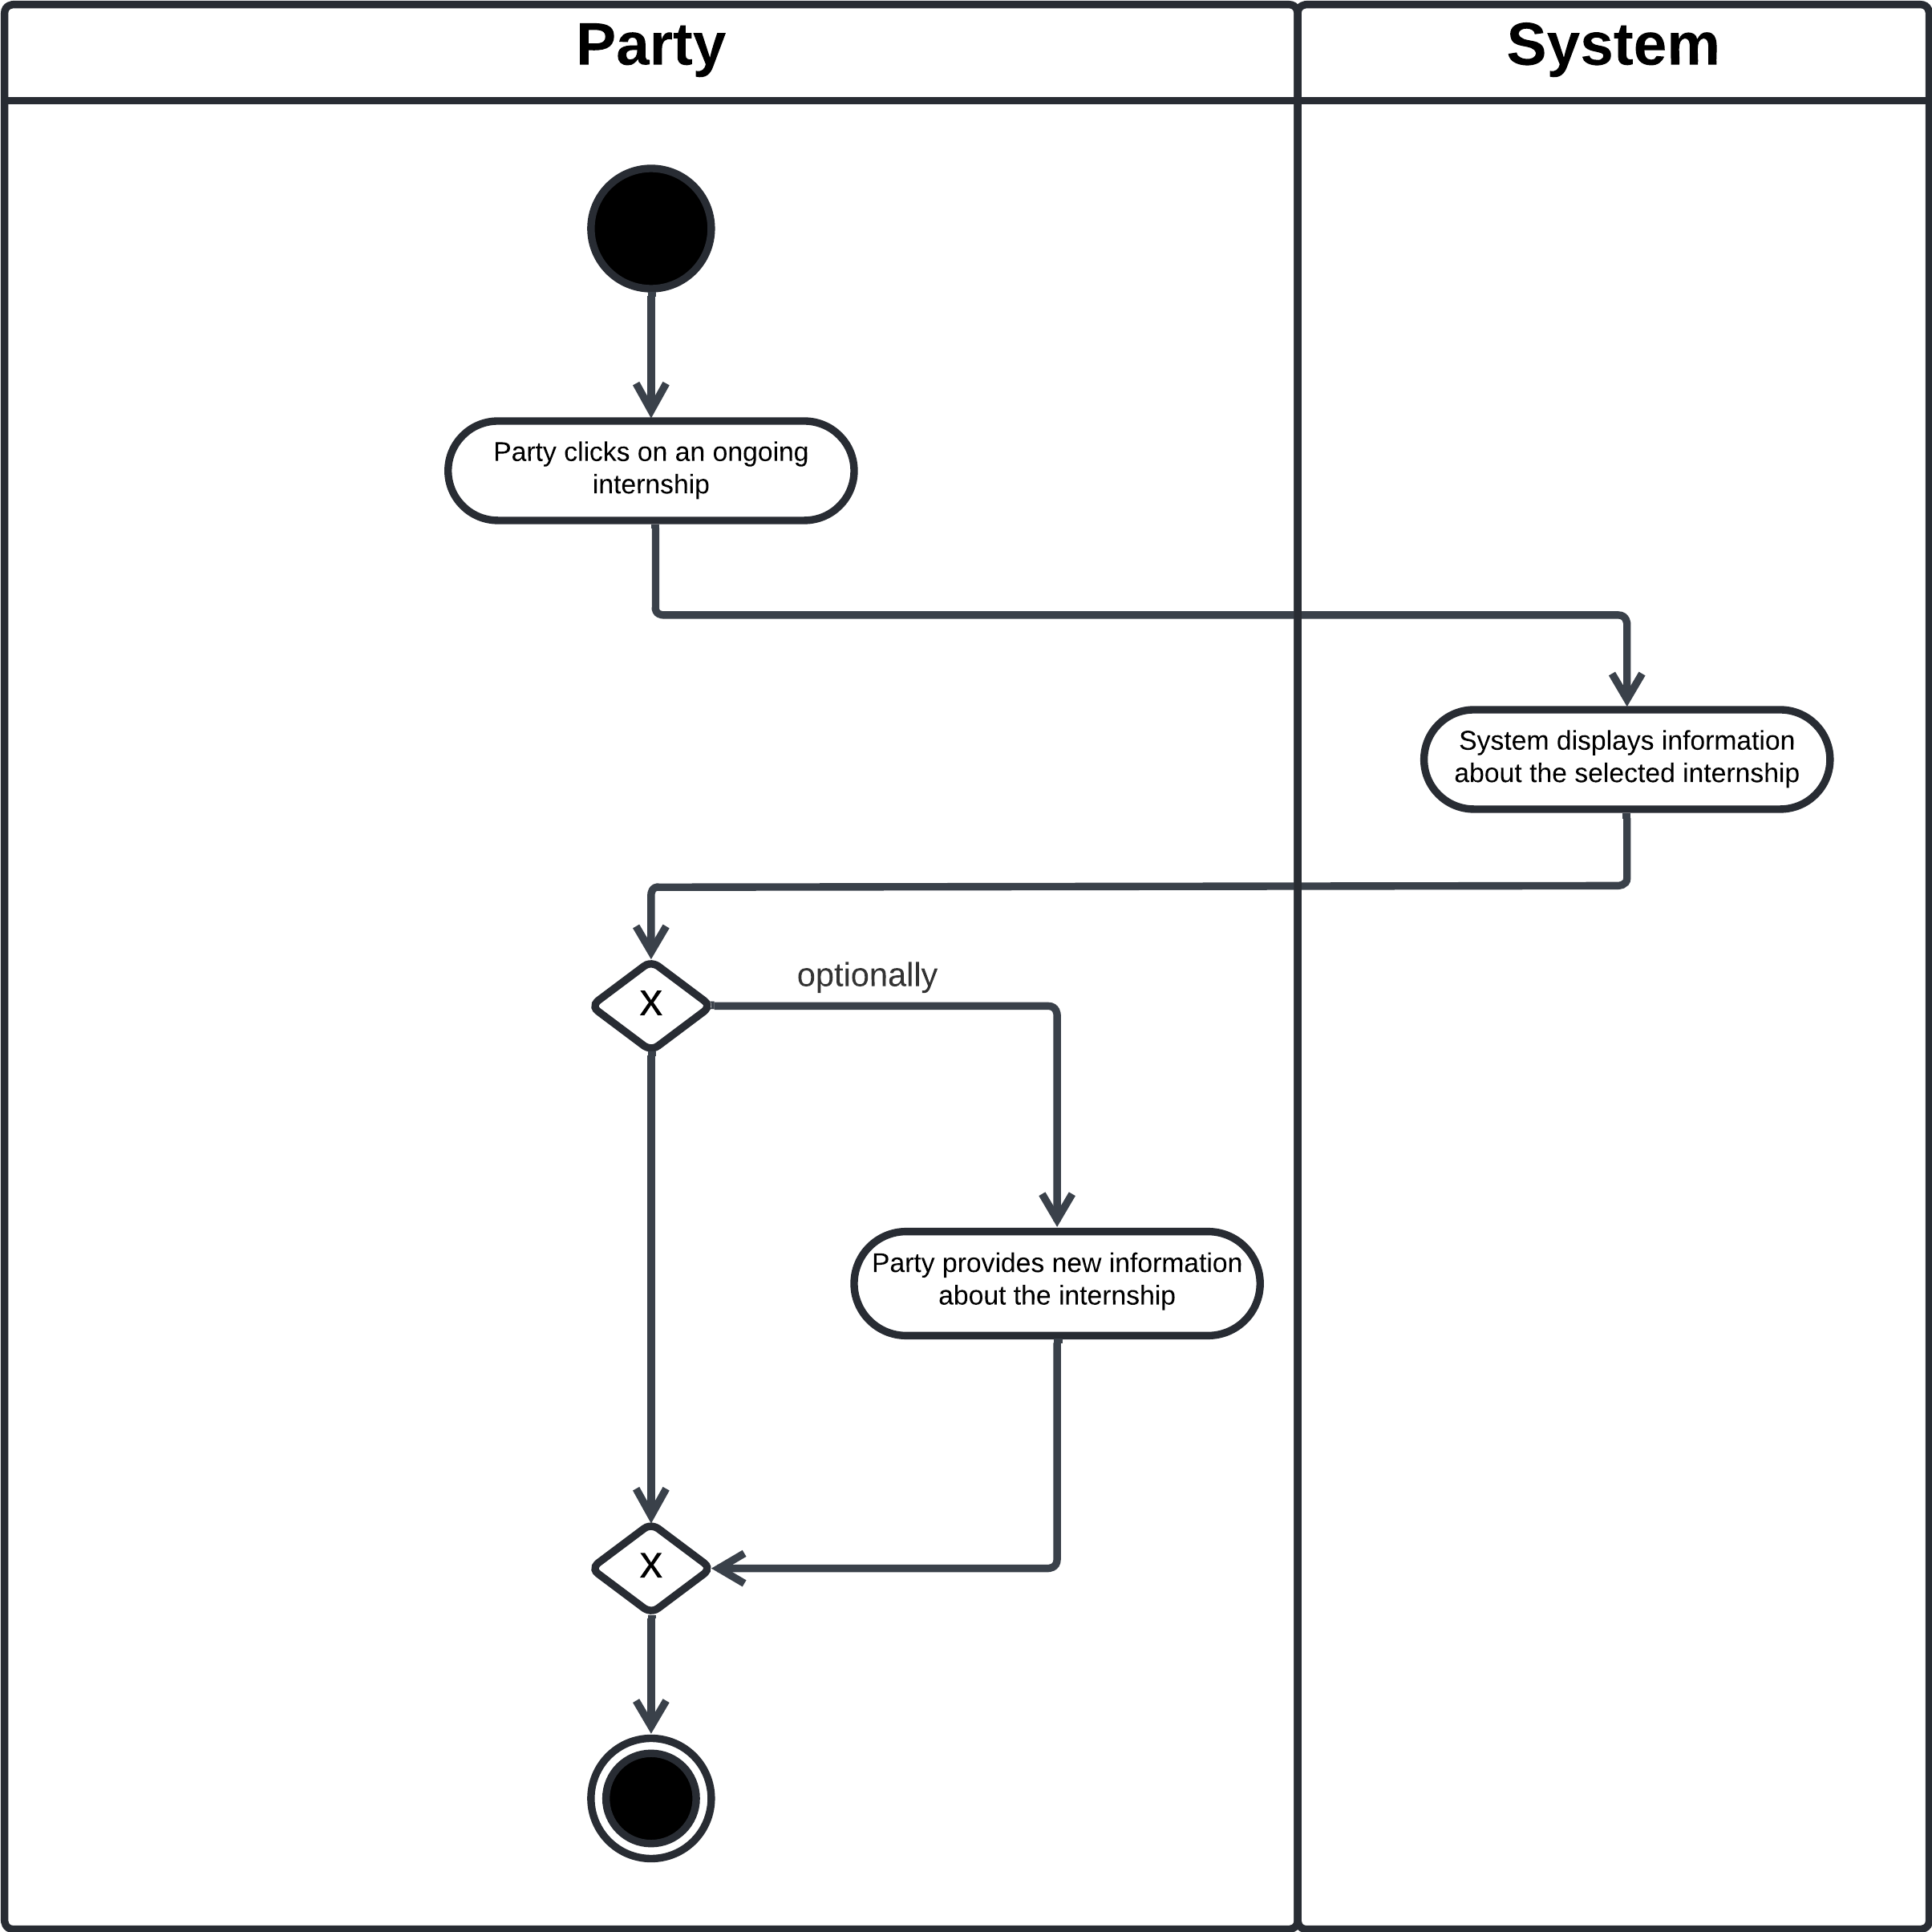
\includegraphics[width=1\linewidth]{LaTeXCode/images/activity diagram/UC15.png}
         \caption{Provide Information for an ongoing Internship}
         \label{fig:provide_information_ongoing_ad}%
     \end{center}
\end{figure}

\newpage

\subsubsection*{UC\cuc . Monitor an ongoing Internship}
\begin{center}
    \begin{longtable}{|l|p{0.75\linewidth}|}
        \hline
        \textbf{Actor}            & Party \\
        \hline
        \textbf{Entry Conditions} & The Party is logged into the S\&C platform and is actively involved in at least an ongoing internship. \\
        \hline
        \textbf{Flow of Events}       
        & \cucsteps. In the dashboard, the Party clicks on an ongoing internship offer in which it is actively participating, entering that internship's page. \\
        & \cucsteps. The system displays all the information about the selected internship. \\
        & \cucsteps. Optionally, the Party provides new information about the internship offer via the \hyperref[subsec: provide_information_ongoing_uc]{\uline{UC. Provide Information for an ongoing Internship}} functionality. \\
        \hline
        \textbf{Exit Conditions}   & The system displays all the information about the selected ongoing internship. \\
        \hline
        \textbf{Exceptions}       & None \\
        \hline
    \end{longtable}
\end{center}

\begin{figure}[H]
    \begin{center}
         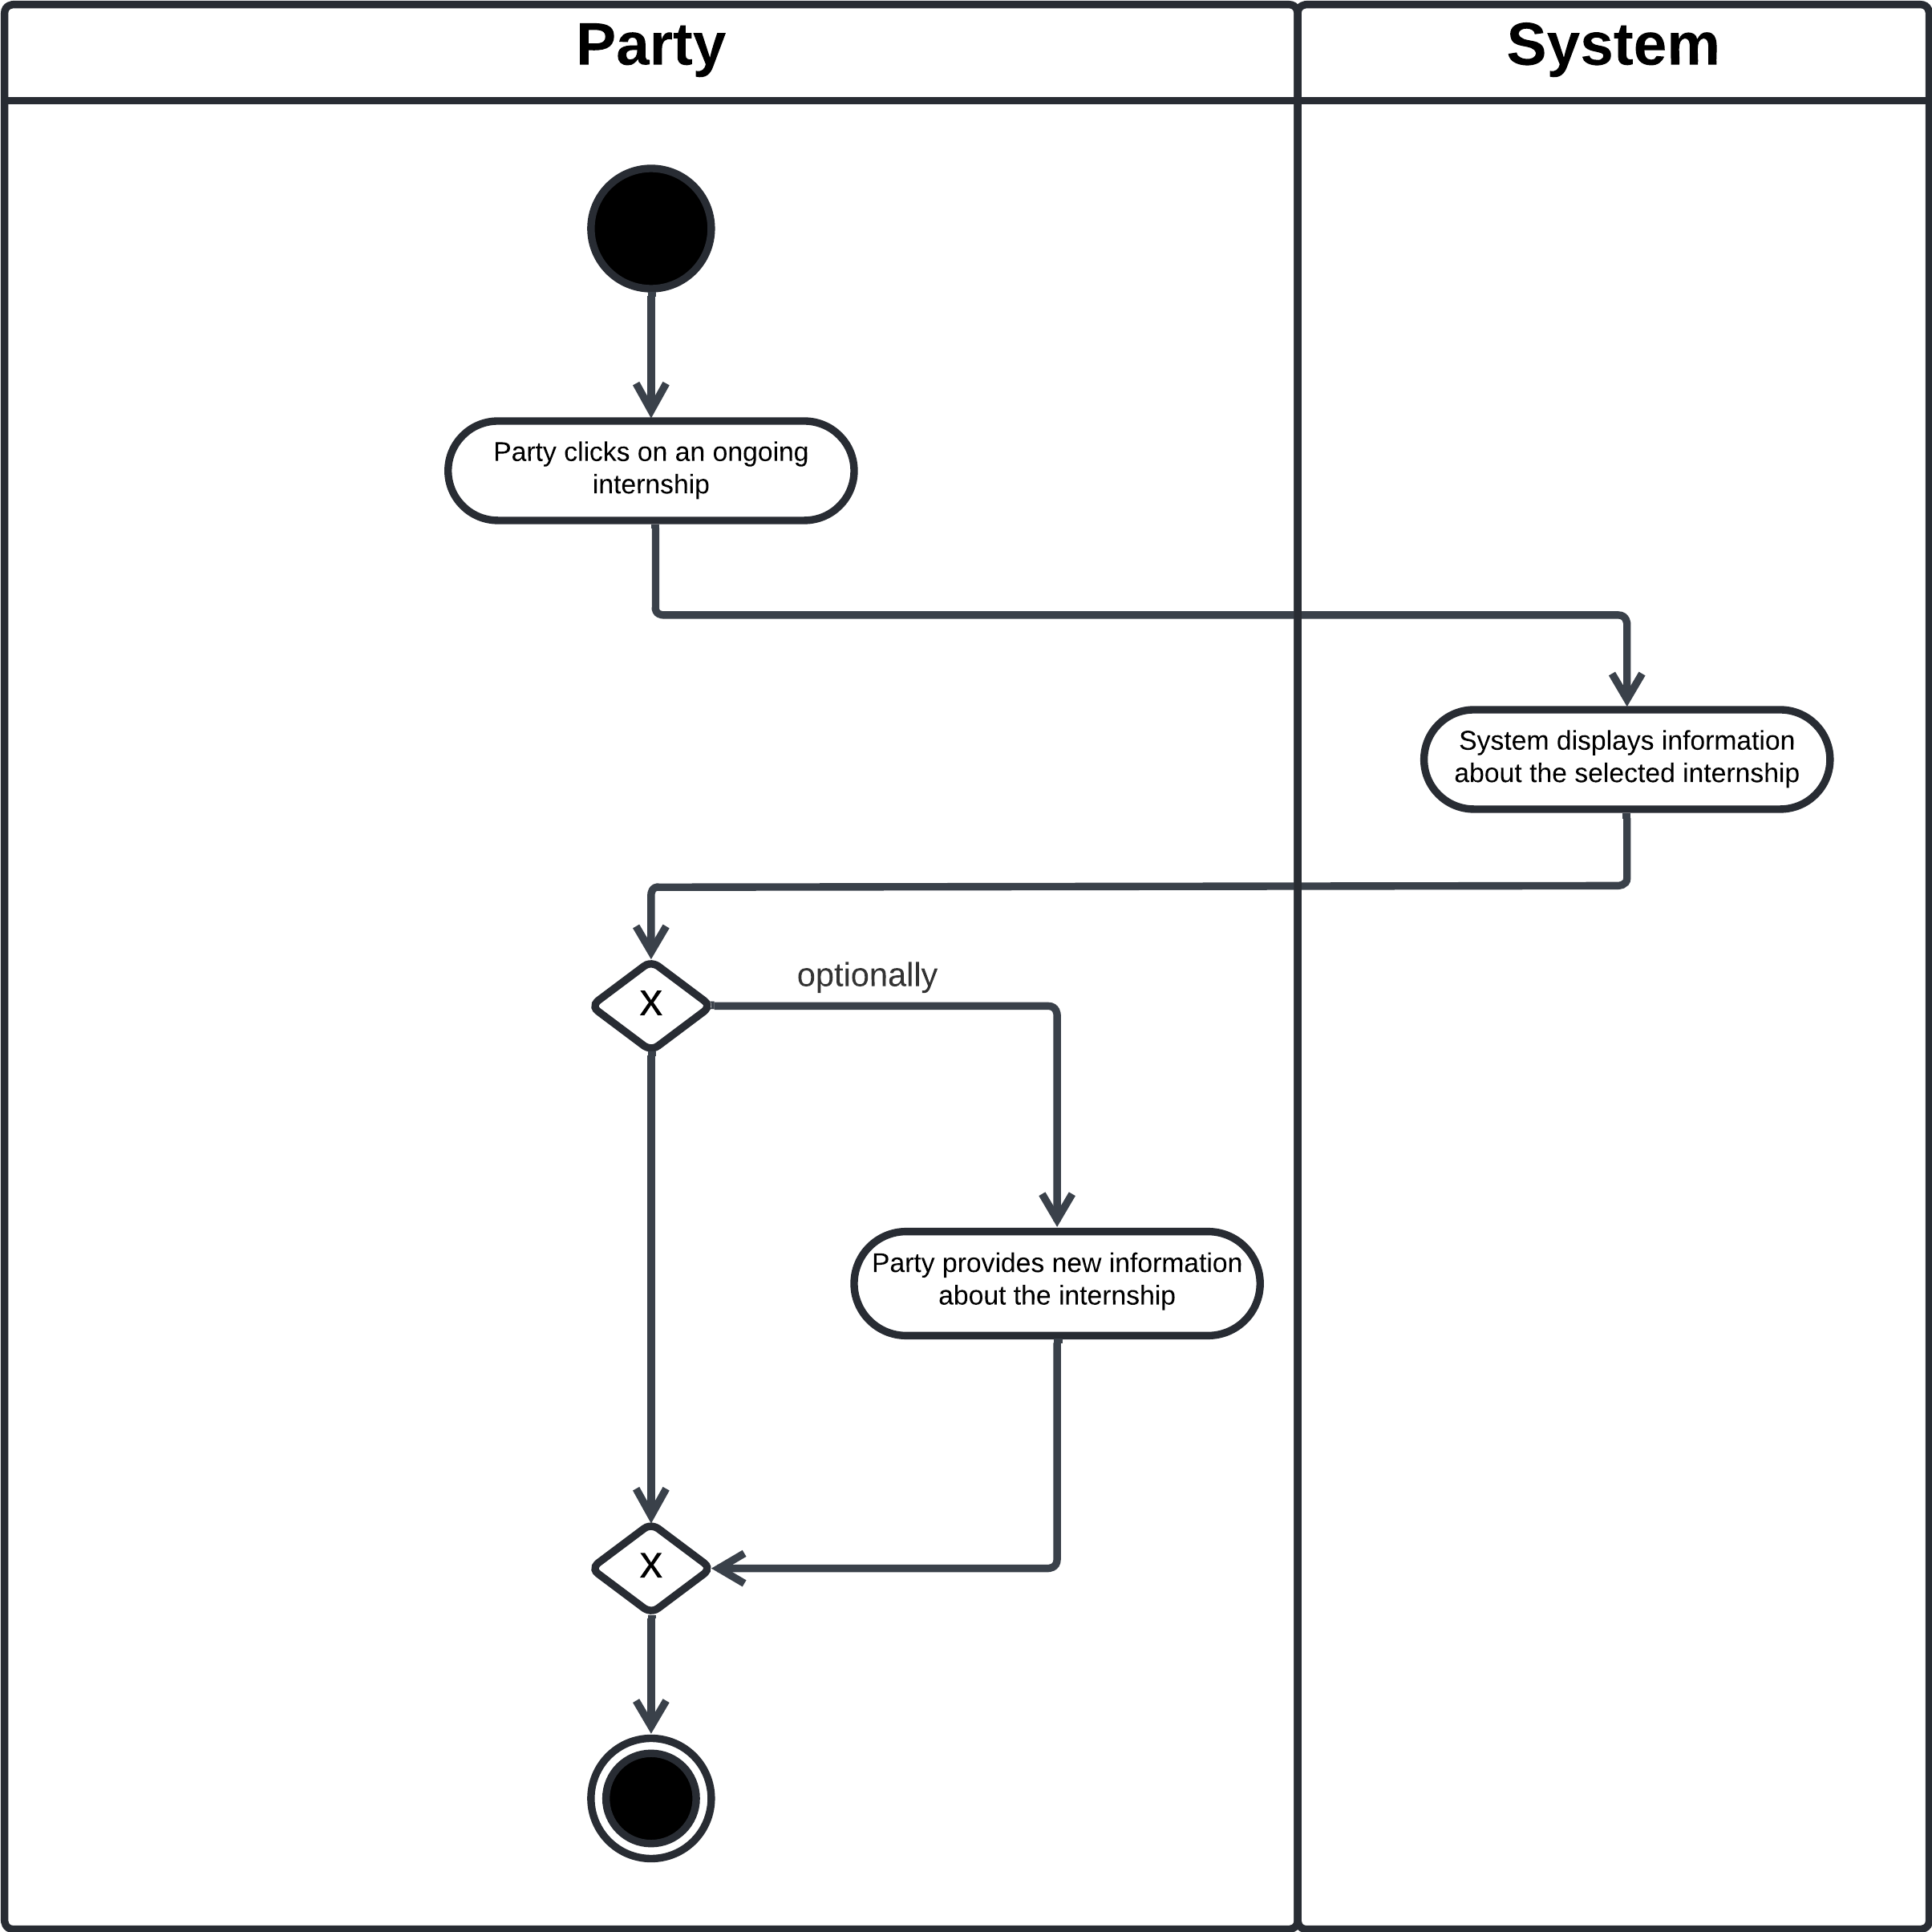
\includegraphics[width=1\linewidth]{LaTeXCode/images/activity diagram/UC15.png}
         \caption{Monitor an ongoing Internship}
         \label{fig:monitor_internship_ad}%
     \end{center}
\end{figure}

\newpage

\subsubsection*{UC\cuc . Report Problems during an Internship}
\begin{center}
    \begin{longtable}{|l|p{0.75\linewidth}|}
        \hline
        \textbf{Actor}            & Party (Student or Company) \\
        \hline
        \textbf{Entry Conditions} & The Party is logged into the S\&C platform, is actively involved in an internship and has identified an issue requiring intervention. \\
        \hline
        \textbf{Flow of Events}       
        & \cucsteps. In the dashboard, the Party navigates to the "Report Problems" section.\\ 
        & \cucsteps. The Party provides a detailed description of the issue, providing:
        \begin{itemize}
            \item Nature of the problem.
            \item Relevant details about when and how the issue occurred.
            \item Optionally, attachments as images or documents to further describe the problem.
        \end{itemize} \\
        & \cucsteps. The Party submits the problem report by clicking the "Report" button.\\ 
        & \cucsteps. The system forwards the Party's report to the Student's University. \\ 
        \hline
        \textbf{Exit Conditions}   & The issue reported by the Party is registered in the system and made available to the University. \\       
        \hline
        \textbf{Exceptions}       & \begin{itemize}
            \item Some mandatory fields are missing: the system doesn't allow the Party to complete the procedure until all the mandatory fields are filled out.
        \end{itemize} \\
        \hline
    \end{longtable}
\end{center}

\begin{figure}[H]
    \begin{center}
         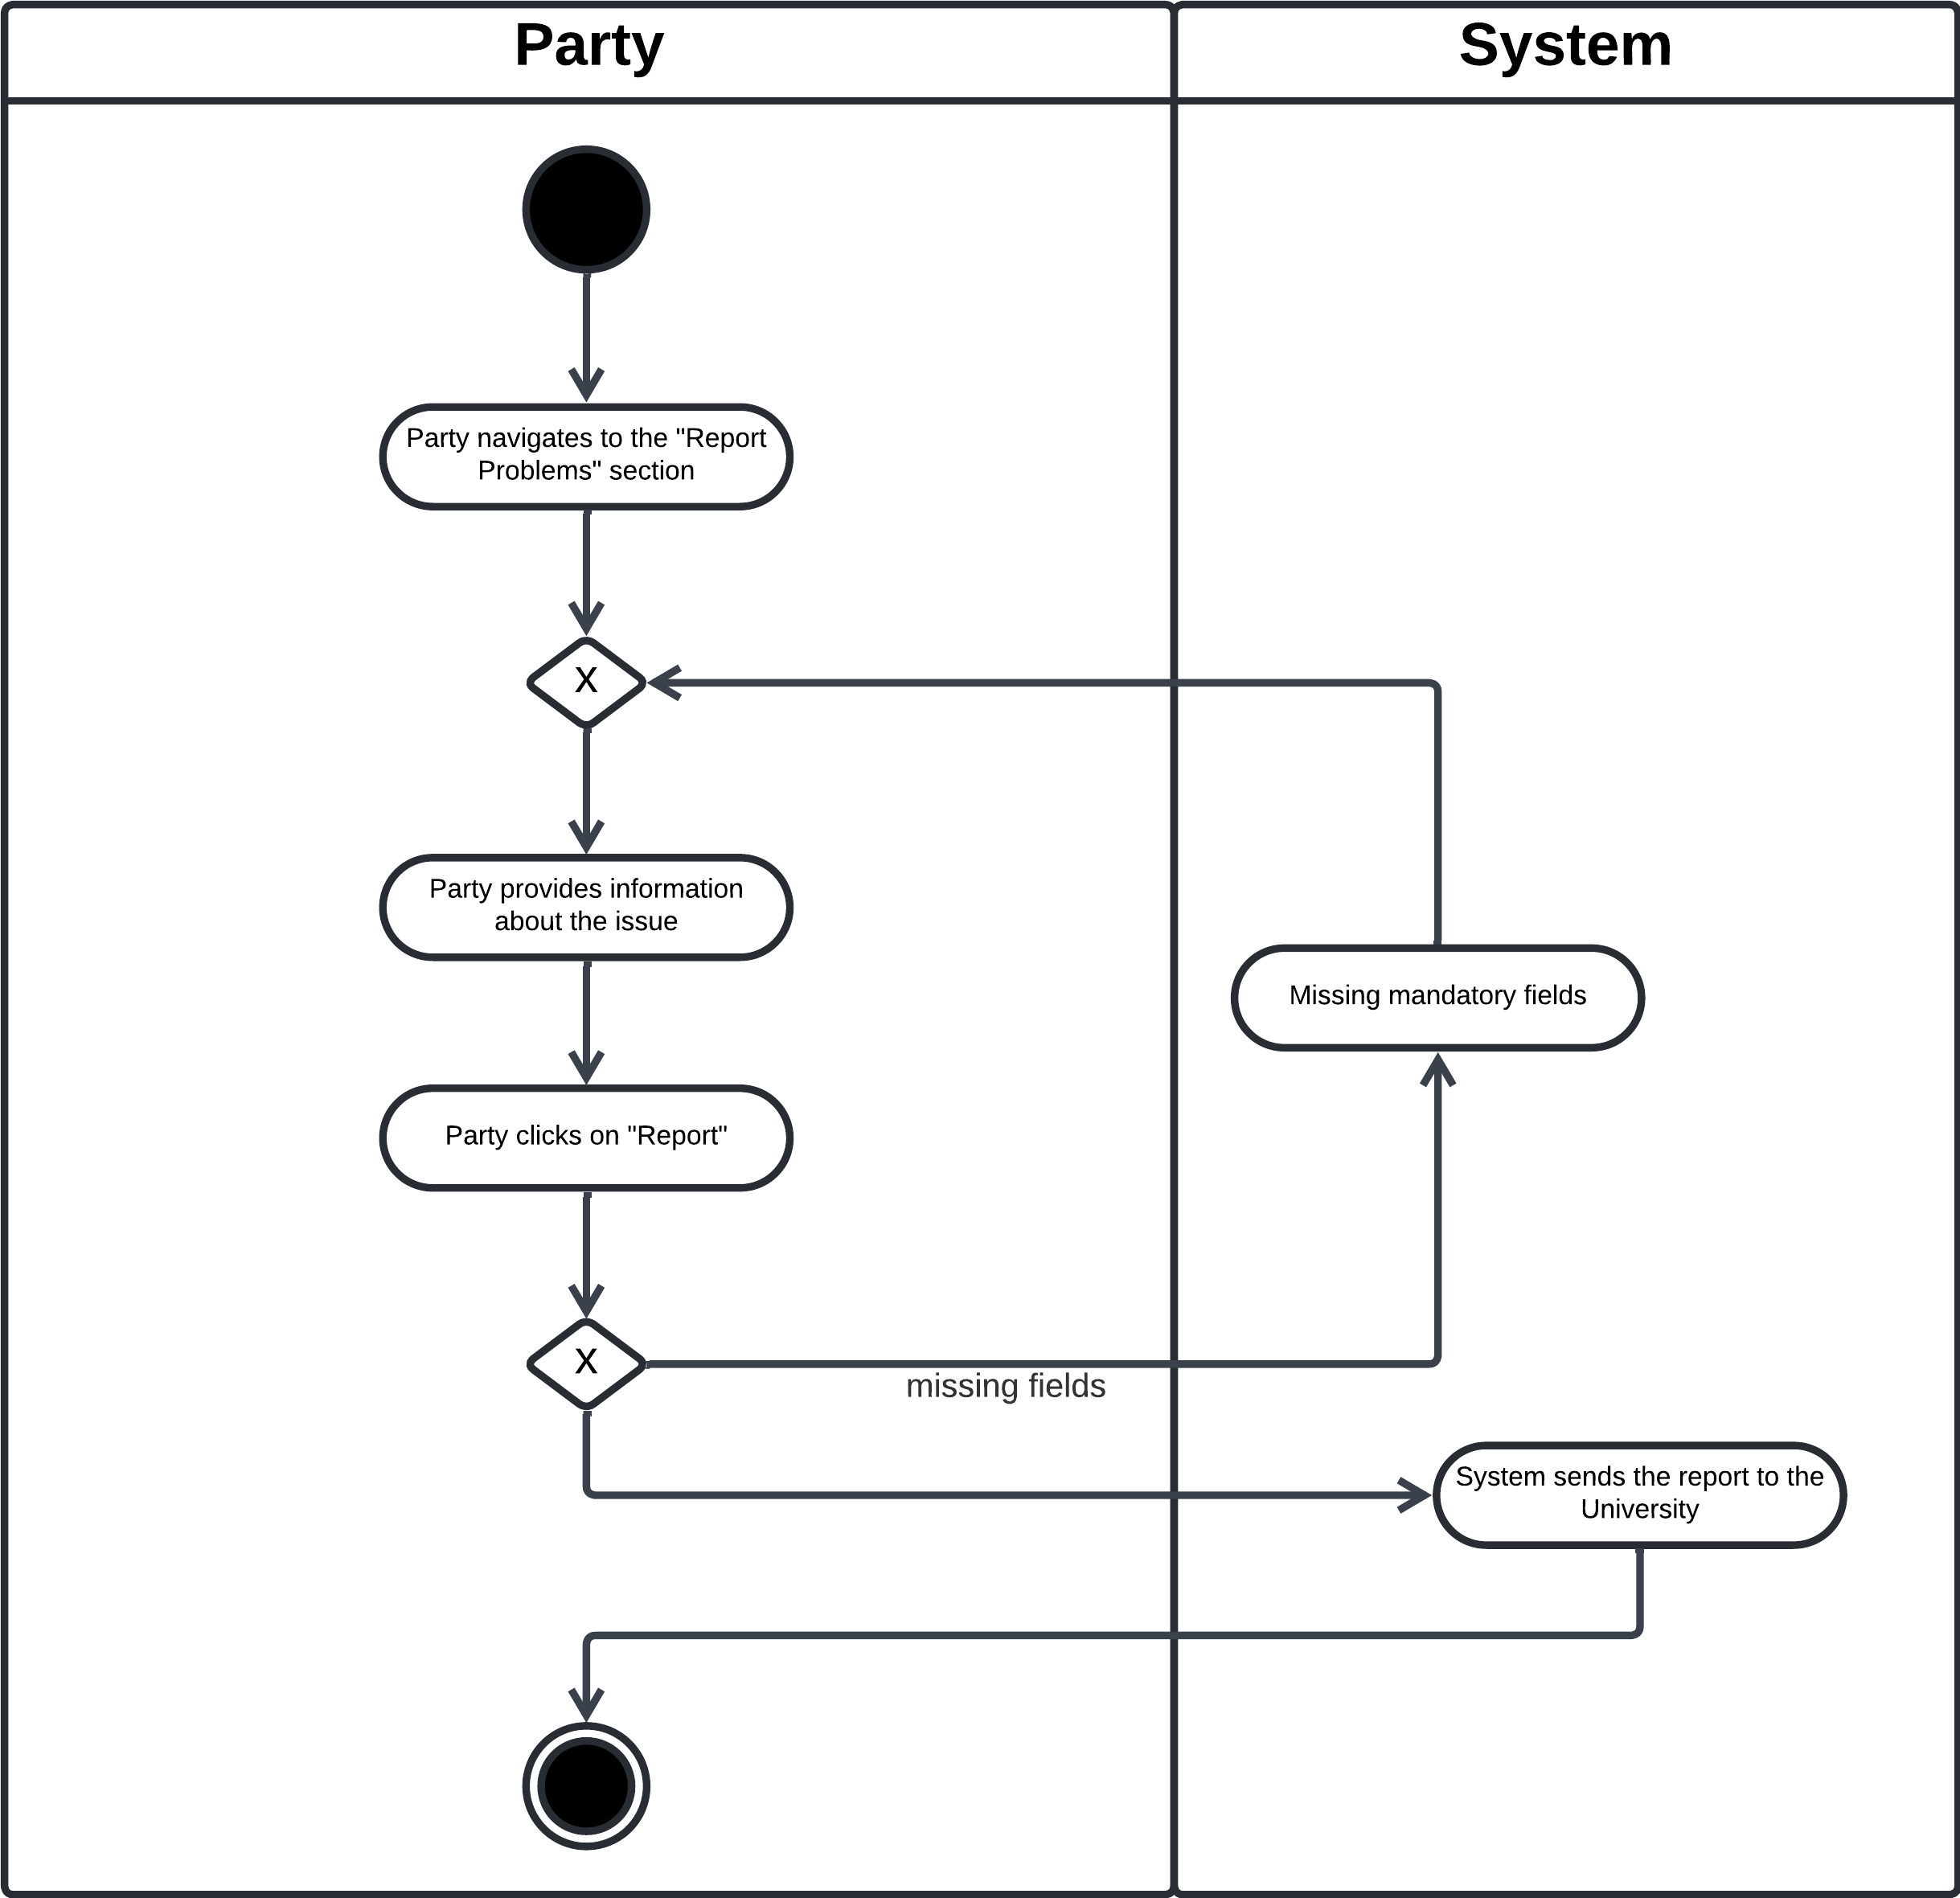
\includegraphics[width=1\linewidth]{LaTeXCode/images/activity diagram/UC16.png}
         \caption{Report Problems during an Internship}
         \label{fig:report_problems_ad}
     \end{center}
\end{figure}

\newpage

\subsubsection*{UC\cuc . Handle Problems during an Internship}
\begin{center}
    \begin{longtable}{|l|p{0.75\linewidth}|}
        \hline
        \textbf{Actor}            & University\\
        \hline
        \textbf{Entry Conditions} & The University is logged into the S\&C platform and one of the Parties involved in an internship concerning one of their students has reported a problem. \\
        \hline
        \textbf{Flow of Events}       
        & \cucsteps. In the dashboard, the University navigates to the "Complaint Management" section. \\ 
        & \cucsteps. The University selects a specific problem report and reviews the details to understand the problem, also visualizing the attached media. \\
        & \cucsteps. The University updates the status of the reported problem in the system, marking it as "In Progress".\\
        & \cucsteps. The University communicates outside the platform with the involved Parties to gather additional information and work collaboratively to resolve the issue. \\
        & \cucsteps. Based on the outcome, the University writes an update associated with the reported problem in the system.\\
        & \cucsteps. The University updates the status of the reported problem in the system, marking it as "Solved".\\
        & \cucsteps. Optionally, the University hides the reported problem in the system, cleaning the unnecessary clutter.\\
        \hline
        \textbf{Exit Conditions}   & The issue previously reported by the Party is formally addressed by the University and the report is updated accordingly in the system. \\       
        \hline
        \textbf{Exceptions}       & None \\
        \hline
    \end{longtable}
\end{center}

\begin{figure}[H]
    \begin{center}
         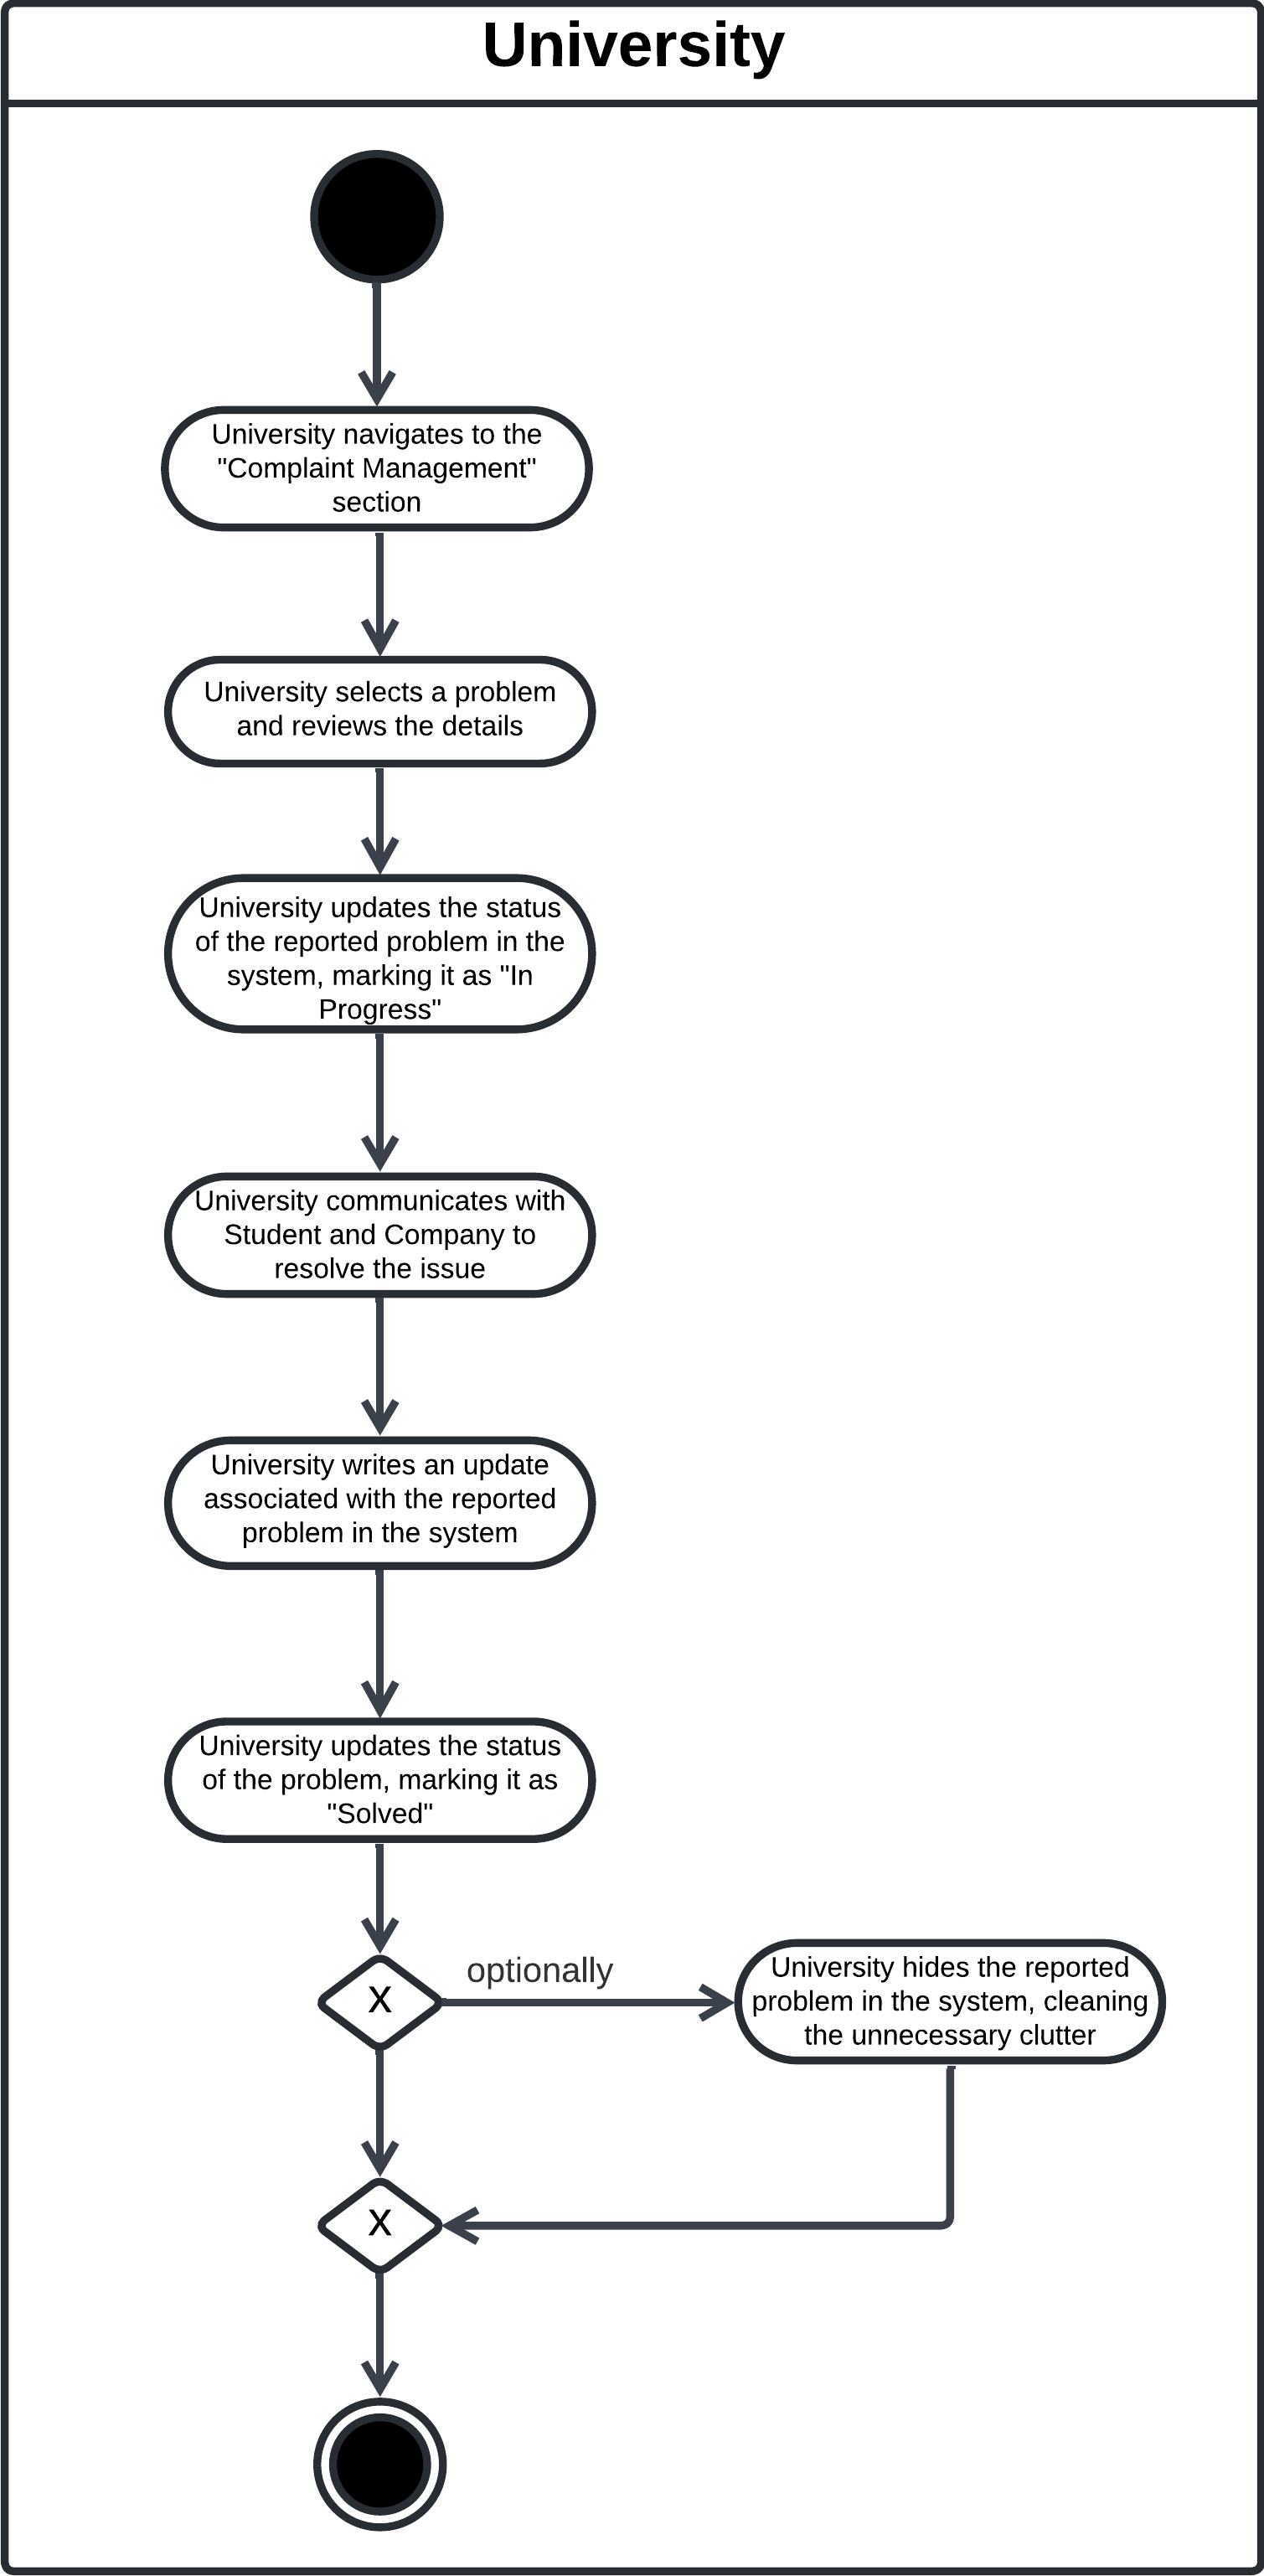
\includegraphics[width=0.65\linewidth]{LaTeXCode/images/activity diagram/UC17.png}
         \caption{Handle Problems during an Internship}
         \label{fig:handle_problems_ad}
     \end{center}
\end{figure}

\newpage

\subsubsection*{UC\cuc . Report Feedback after an Internship}
\begin{center}
    \begin{longtable}{|l|p{0.75\linewidth}|}
        \hline
        \textbf{Actor}            & Party (Student or Company) \\
        \hline
        \textbf{Entry Conditions} & The Party is logged into the S\&C platform and they have been actively involved in a finished internship. \\
        \hline
        \textbf{Flow of Events}       
        & \cucsteps. A non-mandatory survey appears in the Party's dashboard, asking to provide detailed information about the internship to feed the statistical analysis and improve the recommendation algorithm. \\ 
        & \cucsteps. The Party fills out the survey replying to each question. \\
        & \cucsteps. The Party submits the report by clicking the "Submit" button. \\ 
        \hline
        \textbf{Exit Conditions}   & The feedback provided by the Party is processed for improving the recommendation algorithm and recorded in the system. \\       
        \hline
        \textbf{Exceptions}       & \begin{itemize}
            \item The Party closes the survey without completing it: the system doesn't record any information and displays the Party's dashboard.
        \end{itemize} \\
        \hline
    \end{longtable}
\end{center}

\begin{figure}[H]
    \begin{center}
         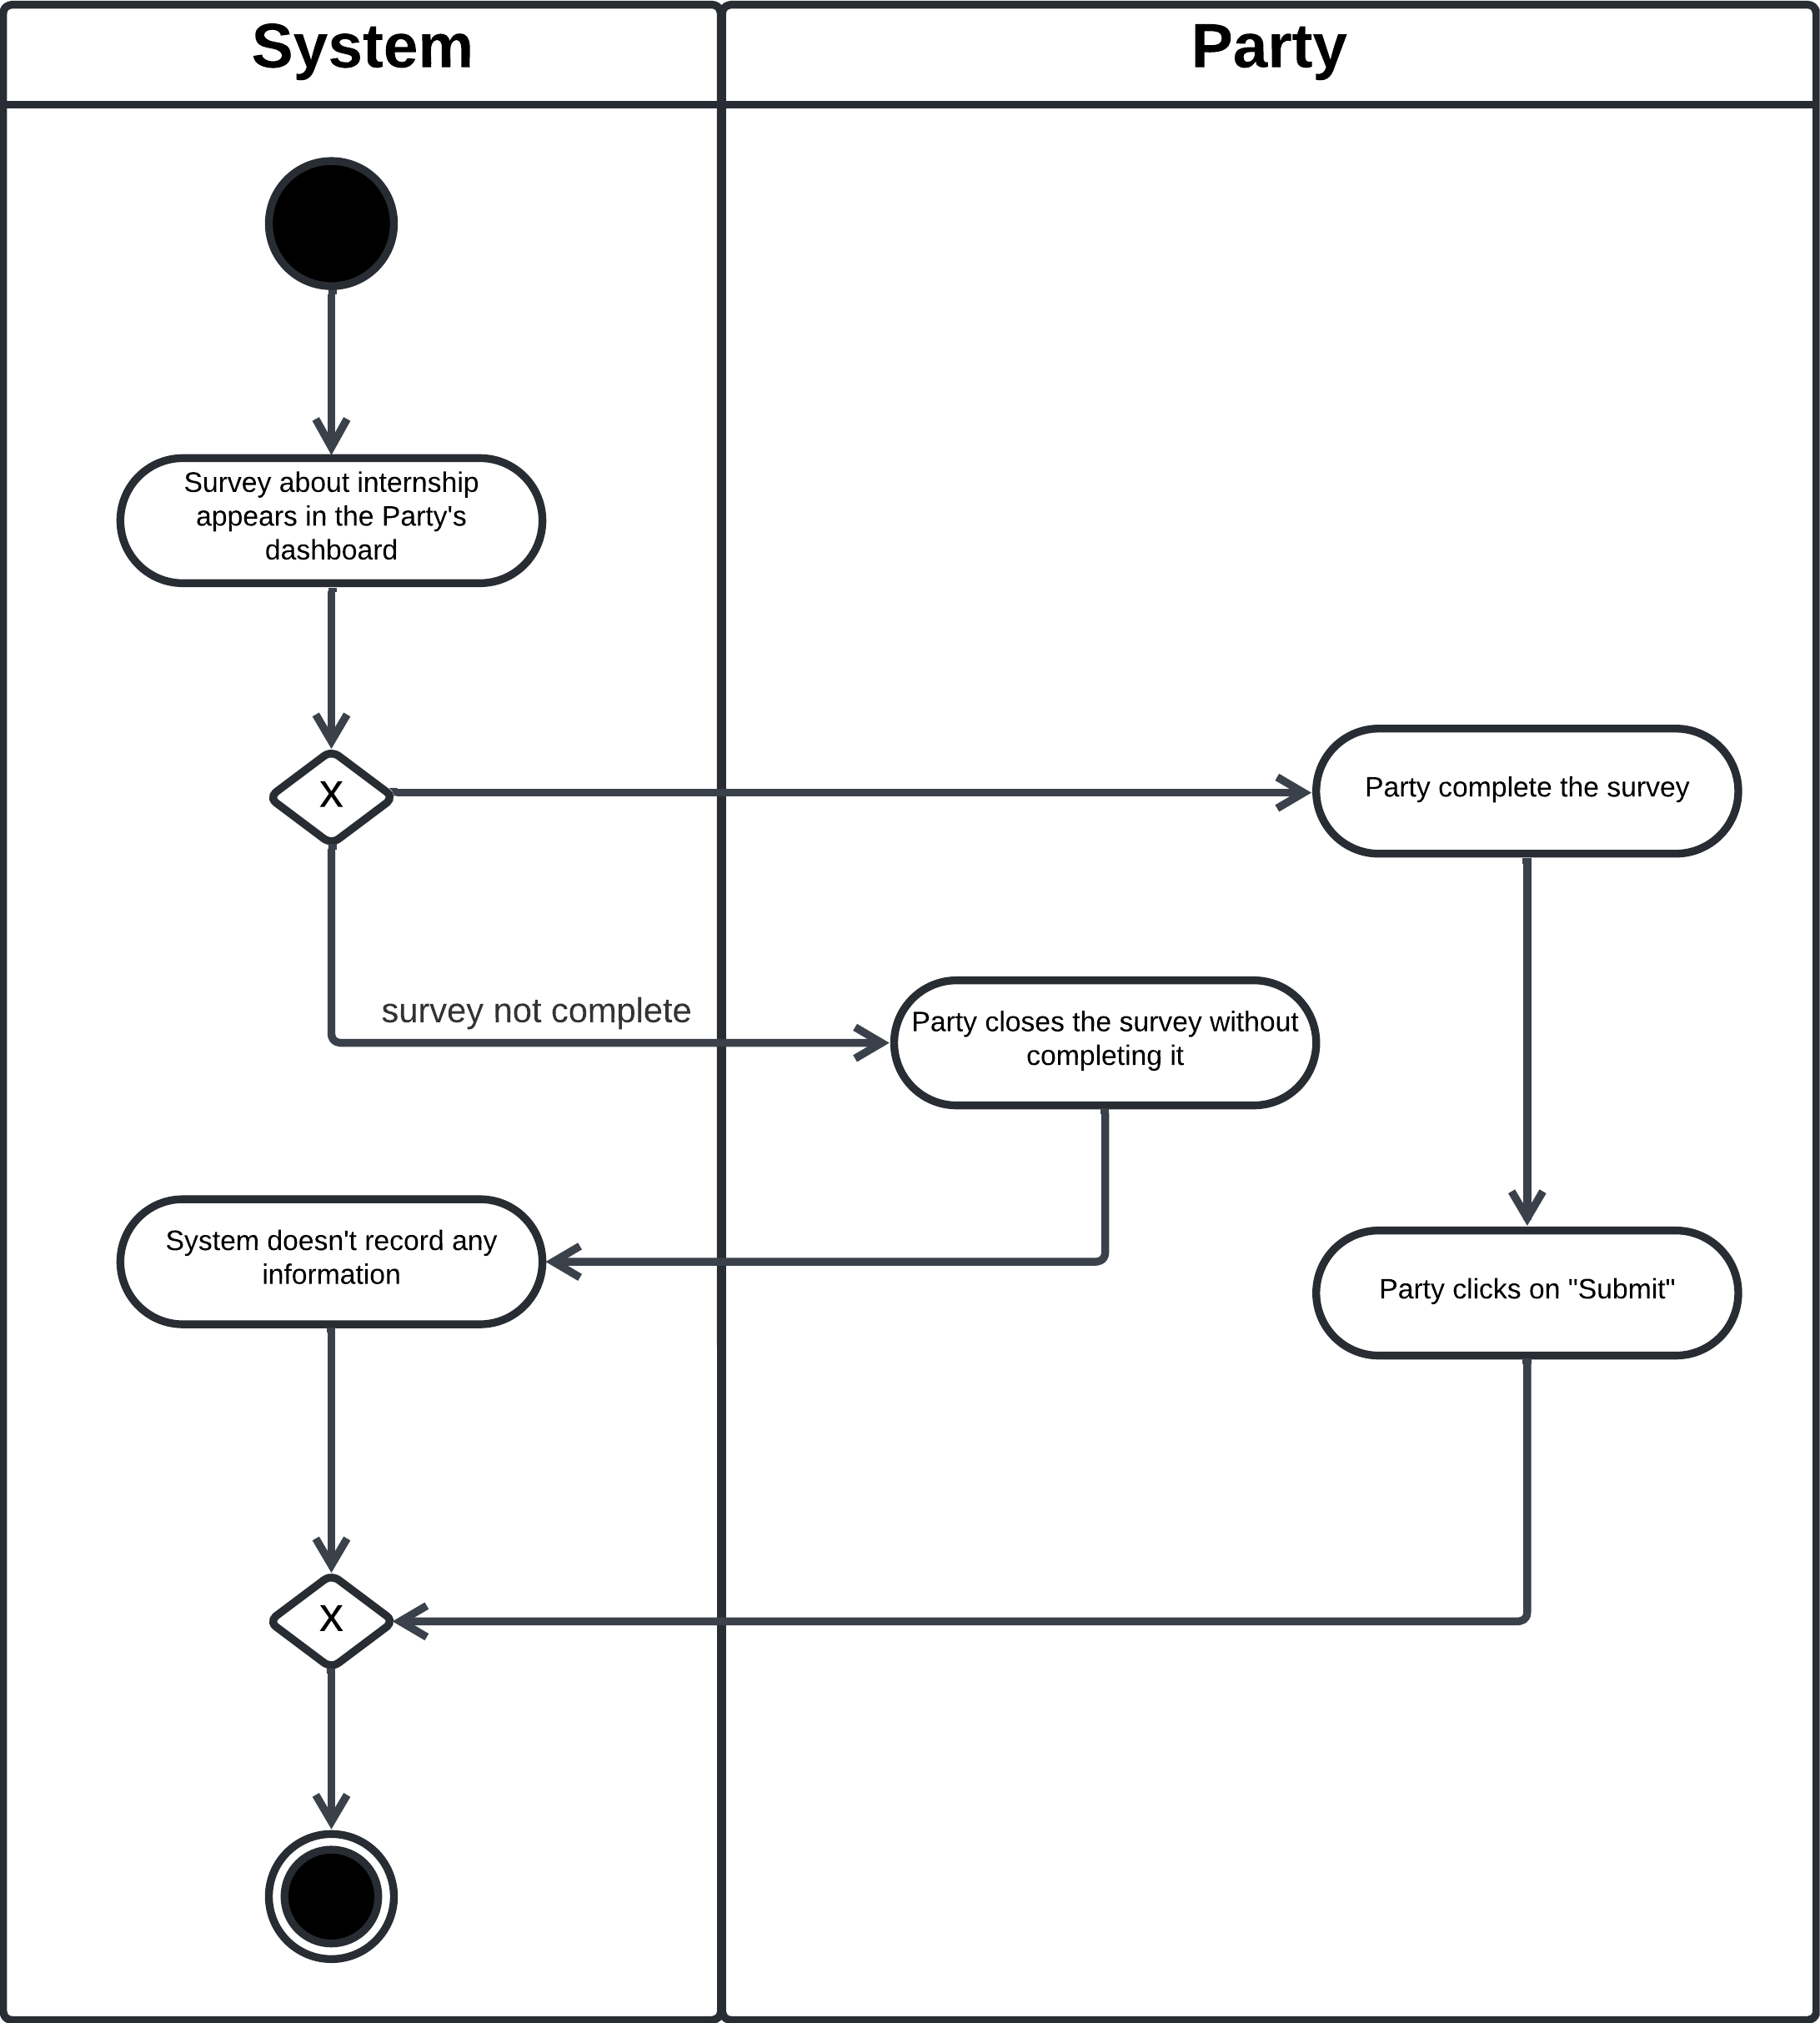
\includegraphics[width=1\linewidth]{LaTeXCode/images/activity diagram/UC18.png}
         \caption{Report Feedback after an Internship}
         \label{fig:report_problems_ad}
     \end{center}
\end{figure}

\newpage

\subsubsection*{UC\cuc . Suggest Optimizations for a Student Profile}
\begin{center}
    \begin{longtable}{|l|p{0.75\linewidth}|}
        \hline
        \textbf{Actor}            & Student\\
        \hline
        \textbf{Entry Conditions} & The Student is logged into the S\&C platform.\\
        \hline
        \textbf{Flow of Events}   
        & \cucsteps. In their "Profile" section, the Student clicks the "Improve Profile" button. \\ 
        & \cucsteps. The system automatically analyzes the student's profile, reviewing the following details:
        \begin{itemize}
            \item Academic background
            \item Skills
            \item Uploaded CV
            \item Certifications and extracurricular activities
        \end{itemize}\\
        & \cucsteps. Based on the analysis, the system generates a list of personalized suggestions to improve the profile which can belong to one of the following categories:
        \begin{itemize}
            \item Add additional skills or certifications.
            \item Update academic details or achievements.
            \item Include or enhance descriptions of projects.
            \item Enhance the overall style by improving clarity or content.
        \end{itemize}\\
        & \cucsteps. The Student reviews the suggestions and eventually decides which one to implement via the  \hyperref[subsec: update_profile_uc]{\uline{UC. Update User Profile}} functionality. \\
        \hline
        \textbf{Exit Conditions}   & The Student's profile is possibly optimized, improving its appeal and relevance for obtaining more internship offers in the future. \\       
        \hline
        \textbf{Exceptions}       & \begin{itemize}
            \item No optimizations can be found: the system doesn't provide any suggestions and terminates silently.
        \end{itemize}\\
        \hline
    \end{longtable}
\end{center}

\begin{figure}[H]
    \begin{center}
         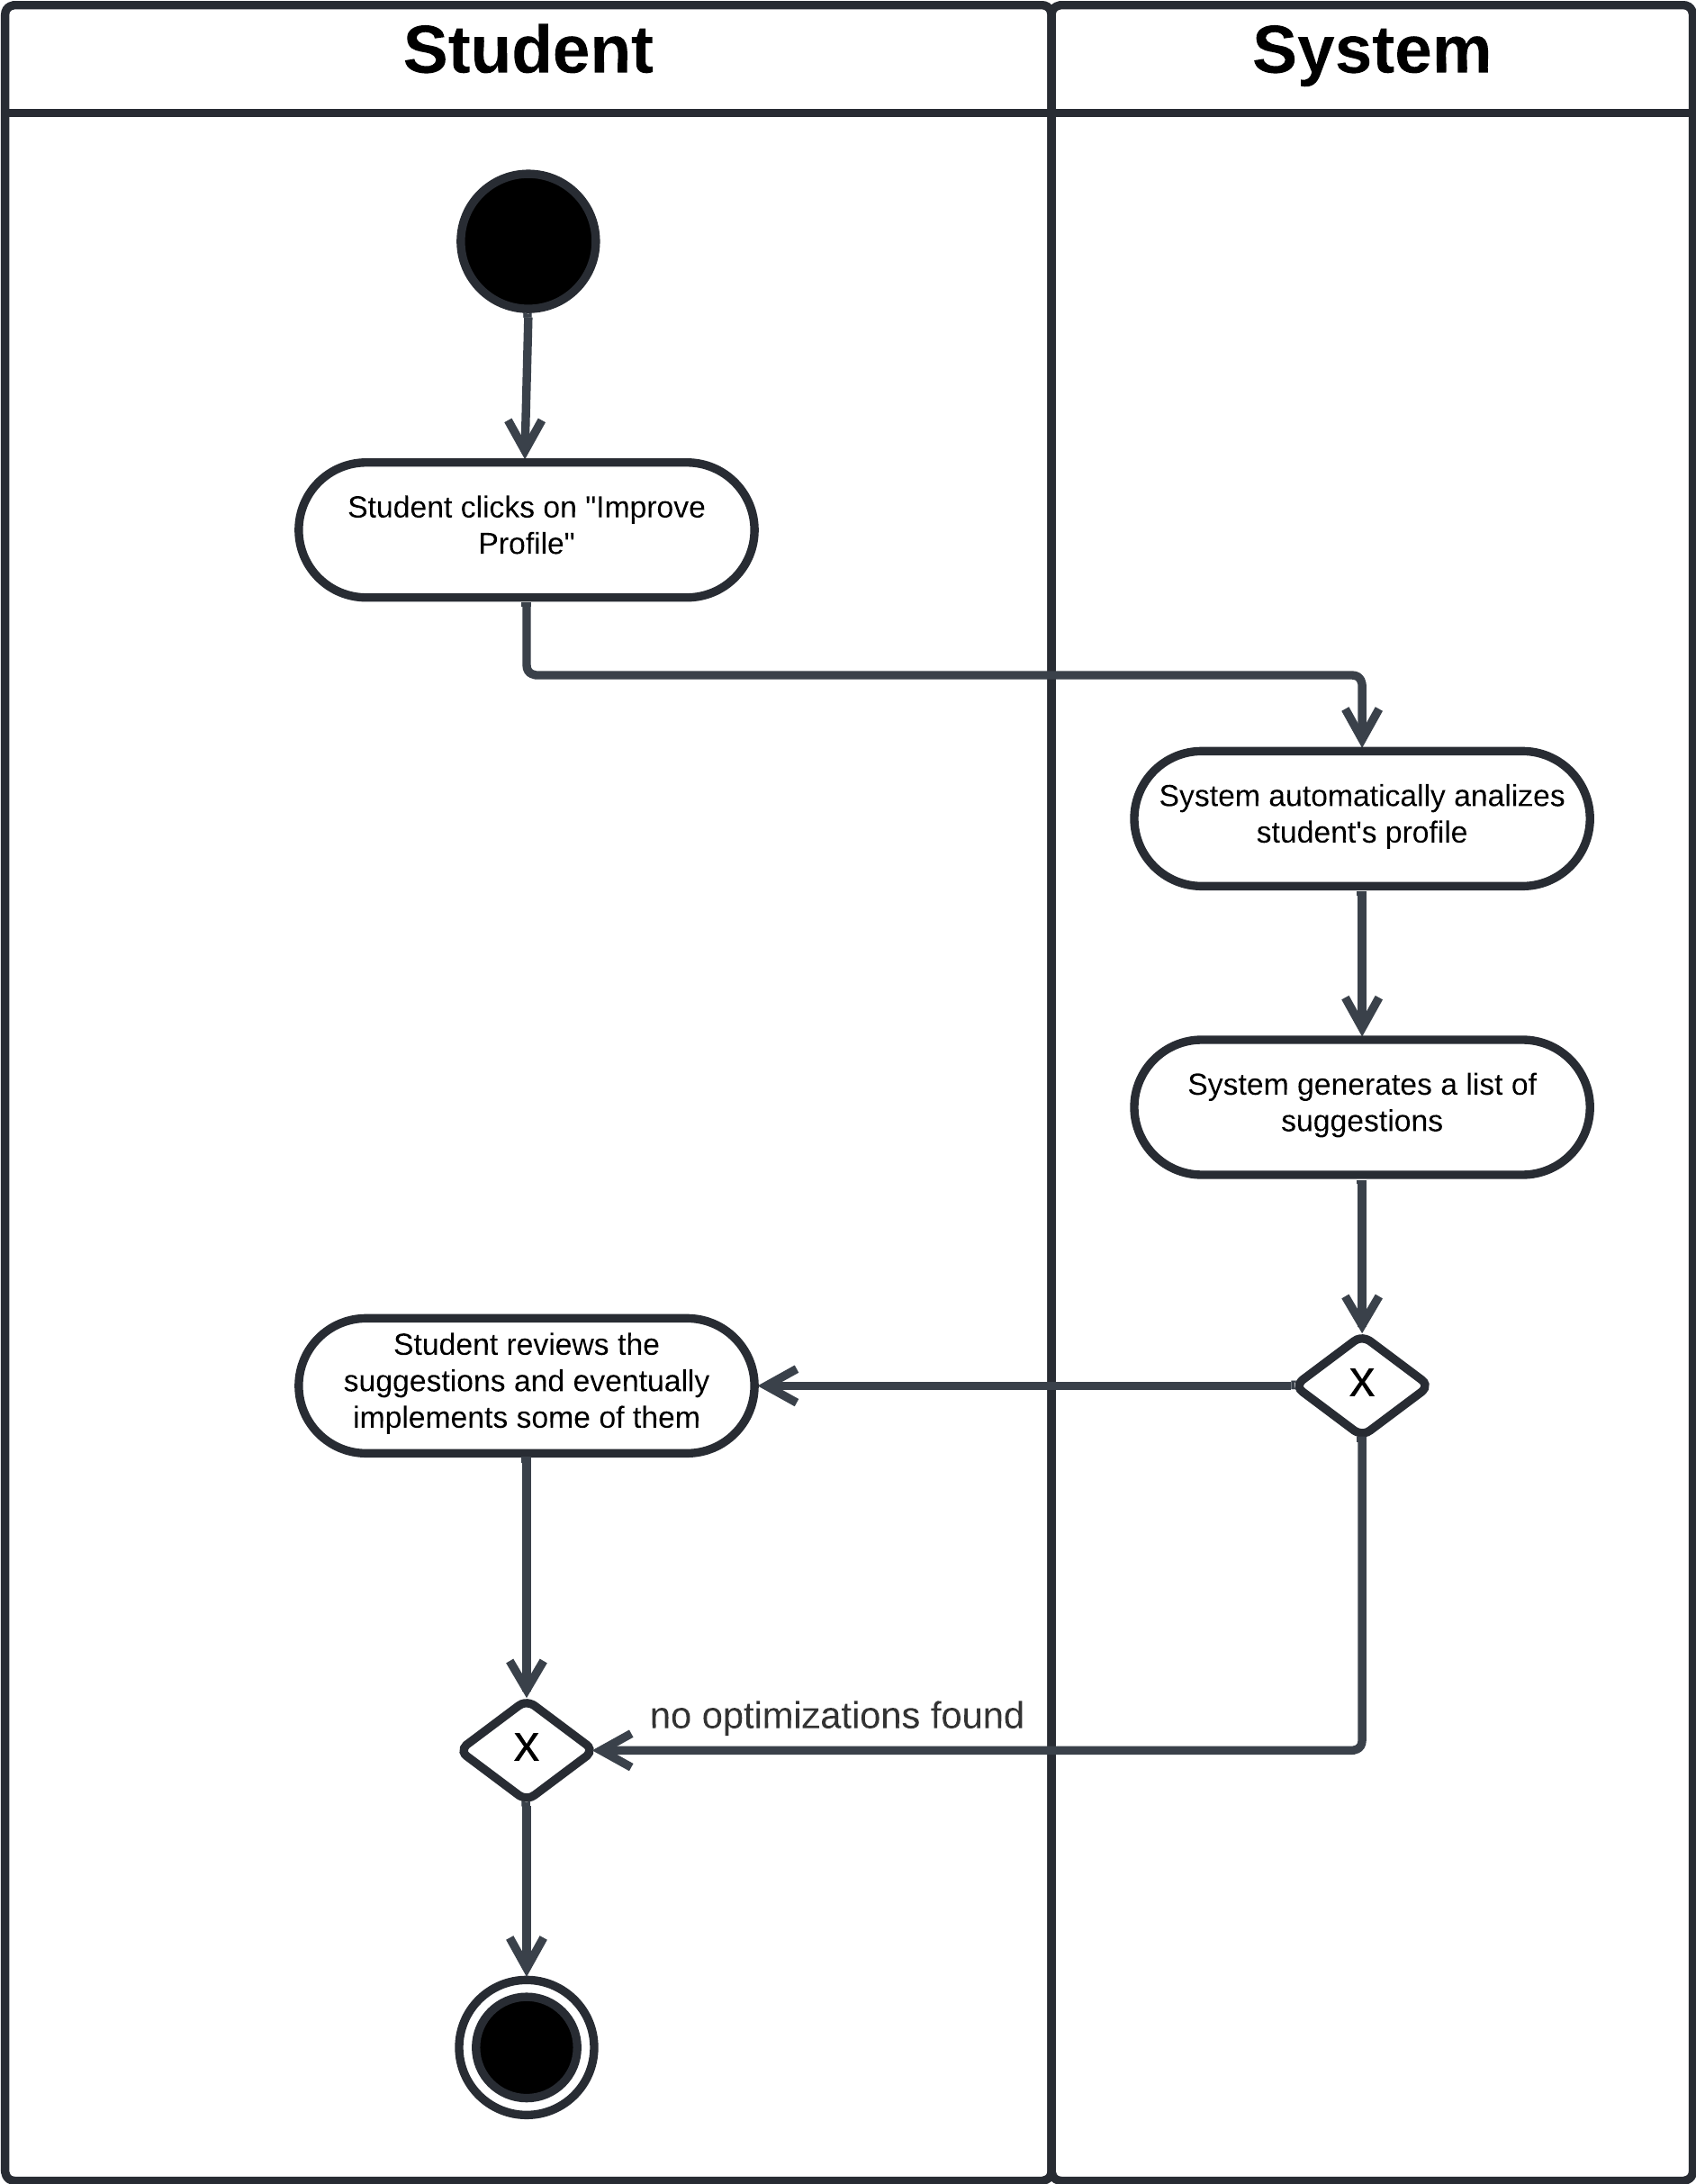
\includegraphics[width=1\linewidth]{LaTeXCode/images/activity diagram/UC19.png}
         \caption{Suggest Optimizations for a Student Profile}
         \label{fig:suggest_optimizations_student_ad}
     \end{center}
\end{figure}

\newpage

\subsubsection*{UC\cuc . Suggest Optimizations for an Internship Offer}
\begin{center}
    \begin{longtable}{|l|p{0.75\linewidth}|}
        \hline
        \textbf{Actor}            & Company \\
        \hline
        \textbf{Entry Conditions} & The Company is logged into the S\&C platform.\\
        \hline
        \textbf{Flow of Events}   
        & \cucsteps. In an internship offer's page, the Company clicks the \newline "Improve Offer" button. \\
        & \cucsteps. The system automatically analyzes the selected internship offer, reviewing the following details:
            \begin{itemize}
                \item Description of the internship
                \item Application domain
                 \item Required skills
            \end{itemize} \\
        & \cucsteps. Based on the analysis, the system generates a list of suggestions to improve the offer:
            \begin{itemize}
                \item Refine the description to better specify tasks and requirements.
                \item Improve the application domain by incorporating additional information or further elaborating on the details already provided."
                \item Introduce or modify the set of required skills.
                \item Enhance the overall style by improving clarity or content.
            \end{itemize} \\
        & \cucsteps. The Company reviews the suggestions and eventually decides which one to implement via the \hyperref[subsec: update_internship_offer_uc]{\uline{UC. Update Internship Offer}} functionality. \\
        \hline
        \textbf{Exit Conditions}   & The Company's selected internship offer is possibly optimized, making it more attractive to students and improving internship visibility for the future.\\       
        \hline
        \textbf{Exceptions}       & \begin{itemize}
            \item No optimizations can be found: the system doesn't provide any suggestions and terminates silently.
        \end{itemize}\\
        \hline
    \end{longtable}
\end{center}

\begin{figure}[H]
    \begin{center}
         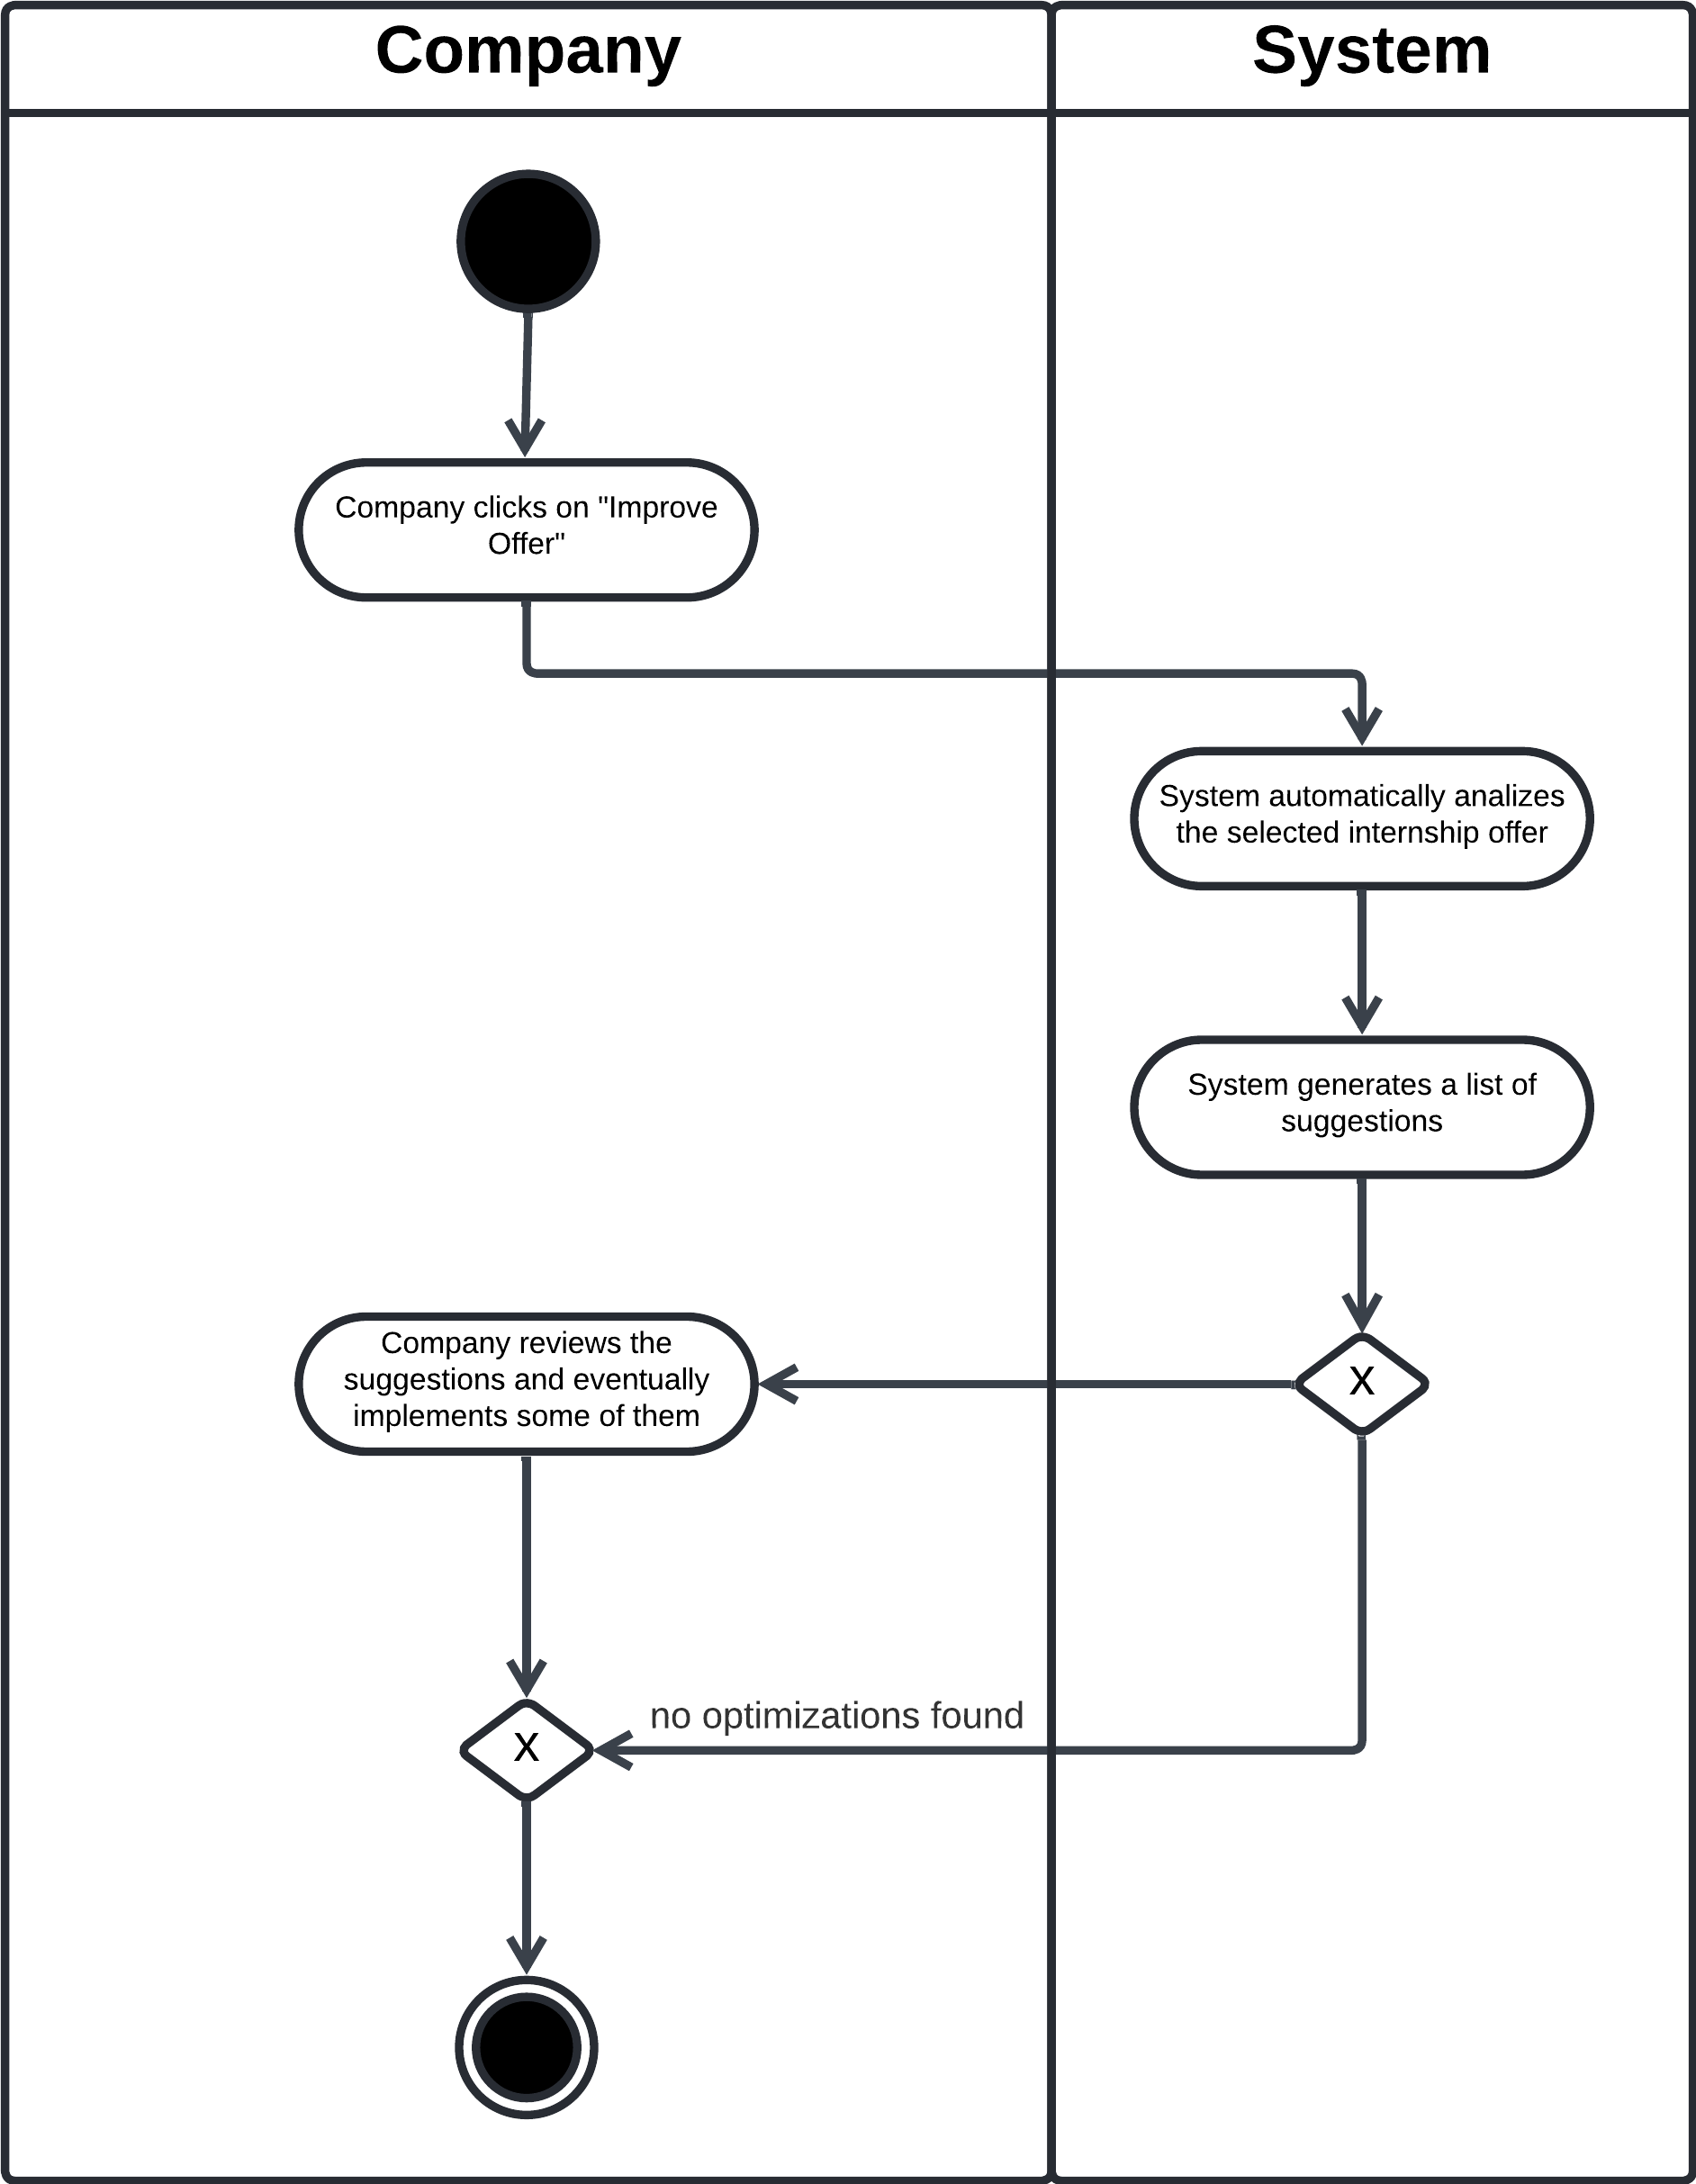
\includegraphics[width=1\linewidth]{LaTeXCode/images/activity diagram/UC20.png}
         \caption{Suggest Optimizations for an Internship Offer}
         \label{fig:suggest_optimizations_internship_ad}
     \end{center}
\end{figure}

\newpage

\subsection{Mapping On Requirements}
\label{subsec:mapping_on_requirements}

\newcounter{row}
\setcounter{row}{1}
\newcommand{\crow} {\therow\stepcounter{row}}

    \begin{longtable}{
        |>{\centering\arraybackslash}p{2cm}
        |>{\centering\arraybackslash}p{2cm}
        |>{\centering\arraybackslash}p{5cm}
        |>{\centering\arraybackslash}p{3.5cm}
        |>{\centering\arraybackslash}p{2cm}|
    }
        \hline
        \textbf{Row ID} & \textbf{Goal ID} & \textbf{Req ID} & \textbf{DA ID} & \textbf{UC ID} \\ \hline
        \endfirsthead
        \hline
        \textbf{Row ID} & \textbf{Goal ID} & \textbf{Req ID} & \textbf{DA ID} & \textbf{UC ID} \\ \hline
        \endhead
        \hline
        \endfoot
        \hline
        \endlastfoot
        \crow & G1 & R1, R2, R17 & DA1 to DA6 & UC1 \\ \hline
        \crow & G1 & R1, R2 & DA1 to DA6 & UC2 \\ \hline
        \crow & G1 & R1, R2 & DA1 to DA6 & UC3 \\ \hline
        \crow & G1 to G12 & R2 & DA1, DA7 & UC4 \\ \hline
        \crow & G1 & R3, R18 & DA1 to DA6 & UC5 \\ \hline
        \crow & G2 & R4, R5, R16 & DA1, DA7 & UC6 \\ \hline
        \crow & G2 & R2, R6, R7, R14, R15, R20, R21 & DA1, DA7 & UC7 \\ \hline
        \crow & G3 & R2, R8, R9 & DA1, DA8 & UC8 \\ \hline
        \crow & G3 & R2, R10, R11, R12, R13 & DA1, DA8 & UC9 \\ \hline
        \crow & G4, G5 & R2, R16, R17, R18, R19, R20, R24, R38 & DA1 & UC10 \\ \hline
        \crow & G4 & R2, R10, R11, R12, R13, R22, R23 & DA1 & UC11 \\ \hline
        \crow & G5 & R2, R16, R22, R24 & DA1 & UC12 \\ \hline
        \crow & G6 & R2, R25, R26, R27, R28, R29, R30, R31 & DA1, DA9, DA10 & UC13 \\ \hline
        \crow & G7 & R2, R32 & DA1, DA11 & UC14 \\ \hline
        \crow & G7 & R2, R33 & DA1, DA11 & UC15 \\ \hline
        \crow & G8 & R2, R34, R35 & DA1, DA12 & UC16 \\ \hline
        \crow & G9 & R2, R36 & DA1, DA13 & UC17 \\ \hline
        \crow & G10 & R2, R37, R38 & DA1, DA14 & UC18 \\ \hline
        \crow & G11 & R2, R39 & DA1 & UC19 \\ \hline
        \crow & G12 & R2, R40 & DA1 & UC20
    \label{tab:traceability}
    \end{longtable}

%We are linking to the UC only the Requirements which involve some concrete step of the UC.E.g. withdraw doesn't interact with UC Apply even if it discards applications

\section{Performance Requirements}
\label{sec:performance_requirements}

As the system does not supply any particular critical functionality to its users, it is acceptable if there are relatively small delays in the system's response times: therefore, constraints about the system's performance are in principle very lax/loose. On the other hand, requirements for the quality of the system are instead tight:

\begin{itemize}
    \item Anytime, the system shall be able to handle a load of up to 10000 concurrent Users without significant performance degradation: however, it shall also be scalable enough for this amount to be increased as a consequence of business decisions which cause the system's scope to widen.
    \item When generating recommendations, both accuracy and F1 score of the mechanisms employed for identifying those recommendations shall be at least 0.8. 
    \item Whenever receiving a request, the system shall respond to the requesting User in less than 5 seconds. This doesn't include recommendations generation, which, however, should be able to be carried out for up to 1.000.000.000 different users.
    \item Whenever any kind of information (including new recommendations, interview invites, or complaints) becomes available to a User, the system shall "append" it to that User's profile in the appropriate section within the following 0.01 seconds, so that it can immediately be shown to that User if they are logged in.
\end{itemize}

\section{Design Constraints}
\label{sec:design_constraints}%

\subsection{Standards Compliance}
\label{sec:standards_compliance}%

This system is designed to adhere to a range of standards and regulations to ensure compliance with legal, technical, and usability requirements. In the following, we outline the primary standards considered:

\begin{enumerate}
\item \textbf{General Data Protection Regulation (GDPR)}
The platform ensures compliance with GDPR to protect users’ personal data. Key measures include:
\begin{itemize}
    \item Data minimization and anonymization techniques for data storage.
    \item Mechanisms for users to access, modify, and delete their data.
    \item Transparent consent collection processes and data usage policies, ensuring that the user is aware on which operations and processes are applied to the shared data.
\end{itemize}
By integrating these security measures, the S\&C platform aims to foster user trust and compliance with current regulations.

\item \textbf{World Wide Web Consortium (W3C)}
The system adheres to W3C standards to ensure interoperability and usability across modern browsers. Some useful target objectives derived from the guidelines are:
\begin{itemize}
    \item Use meaningful HTML elements to structure content properly, enabling assistive technologies to interpret the page effectively.
    \item Follow WAI-ARIA (Web Accessibility Initiative–Accessible Rich Internet Applications) standard, a framework for adding attributes to identify features for user interaction, how they relate to each other, and their current state
    \item Perform decisions in order to reduce load times and enhance responsiveness.
\end{itemize}

\item \textbf{Web Content Accessibility Guidelines (WCAG)}
To ensure accessibility, the system follows the latest WCAG standards, a subset of W3C standard that outlines principles for making web content more accessible for people with disabilities:
\begin{itemize}
    \item Support for assistive technologies: screen readers and magnifiers, speech recognition software, keyboard-only navigation. The majority of the accessibility tools are already provided by the OS; the main focus should be in ensuring that such technologies are fully supported and working while interacting with the system.
    \item Accessible navigation structures and compatibility across various devices and input methods.
\end{itemize}
\end{enumerate}

\subsection{Hardware Limitations}
\label{sec:hardware_limitations}%
Considering the nature of the system, which is a WebApp, hardware limitations are minimal, as the system is designed to be lightweight and operates on standard devices and browsers, requiring only basic hardware specifications.

\section{Software System Attributes}
\label{sec:software_system_attributes}%

The main attributes that the system to be developed shall present are outlined here, listed in order of importance for its correct functioning.

\subsection{Reliability}
\label{sec:reliability}%

The system shall ensure high reliability: namely, it shall handle failures effectively and promptly recover from disruptions, minimizing total downtime, frequency of failures and number of functionalities involved. This shall be achieved by employing standard mechanisms for fault tolerance, such as replication of data storage or back-end computation nodes, ensuring no single point of failure compromises the system.

\subsection{Availability}
\label{sec:availability}%

The system shall guarantee at least a 2-nines availability (99\%, or a total downtime of at most 3.65 days/year), ensuring it is available except for planned maintenance, which should occur outside peak hours and be announced in advance anyway.
The decision is based on the fact that it does not offer any critical service to users that cannot be postponed in time.
A robust monitoring system shall track application health and trigger alerts for any performance issues or downtime.

\subsection{Security}
\label{sec:security}%

The system shall implement secure authentication and authorization mechanisms to verify user identities and restrict access to features based on user roles. Such guarantees may be implemented through strong password policies, 2FA, encrypted communication protocols (e.g., HTTPS), etc.
Additionally, the platform must ensure data integrity by preventing unauthorized modifications and preserving the accuracy of stored information, both physically and virtually.
To uphold confidentiality, the system shall encrypt sensitive data both in transit and at rest, ensuring that data remains unreadable even if intercepted or exposed. Secure data storage practices must be observed.
Moreover, the system must be resilient to common attack vectors, including SQL injection, cross-site scripting (XSS), and cross-site request forgery (CSRF). The platform should also incorporate regular security patches to address newly discovered vulnerabilities.

\subsection{Maintainability}
\label{sec:maintainability}%

System maintenance shall be planned for hardware or software upgrades, or for the deployment of production code containing additional functionalities, bug fixes or security updates. 
It should last 8 hours on average, theoretically enabling it to be carried out entirely outside peak traffic periods; in any case, it shall not exceed 24 hours. 
Maintenance bursts should happen exceptionally, possibly no more than twice or thrice a year, and shall always be announced in advance to the public (minimum 48 hours before). 
Software maintenance shall instead be employed right from the start of the development process by enforcing the application of best practices, in compliance with the industry standards; code shall be clean, modular, reusable, and low-coupled, to facilitate the introduction of new functionalities as needed.

\subsection{Portability}
\label{sec:portability}%

Since the platform is offered as a WebApp, it operates through standard web browsers and inherently supports compatibility across various operating systems.
Given this architecture, there is no need for native application installations, ensuring ease of use and minimizing setup complexity. Therefore, the chosen architecture and platform's reliance on web standards already solves all aspects related to portability.
The architecture of the platform shall be designed to offer portability, ensuring that it can be deployed across various environments and, eventually, hosting services. By utilizing containerization technologies, the application shall be easily migrated regardless of the underlying infrastructure.



    \chapter{Formal Analysis using Alloy}
    \label{ch:formal_analysis_using_alloy}%
    \input{Chapters/4_-_Formal_Analysis_using_Alloy}


    \chapter{Effort Spent}
    \label{ch:effort_spent}%
    \begin{table}[H]
    \begin{center}
        \begin{tabular}{c|c}
            \hline
            Group Member & Effort Spent in each Section \\
            \hline
            Riccardo Piantoni & \begin{tabular}{p{0.25\linewidth}|c}
                             Introduction          & $4h$ \\
                             Overall Description   & $7h$ \\
                             Specific Requirements & $6h$ \\
                             Formal Analysis       & $17h$ \\
                             Reasoning             & $8h$ \\
            \end{tabular} \\
            \hline
            Matteo Rossi & \begin{tabular}{p{0.25\linewidth}|c}
                            Introduction          & $5h$ \\
                            Overall Description   & $8h$ \\
                            Specific Requirements & $16h$ \\
                            Formal Analysis       & $3h$  \\
                            Reasoning             & $6h$ \\
            \end{tabular} \\
            \hline
            Jacopo Sacramone & \begin{tabular}{p{0.25\linewidth}|c}
                            Introduction          & $4h$ \\
                            Overall Description   & $6h$ \\
                            Specific Requirements & $16h$ \\
                            Formal Analysis       & $0h$ \\
                            Reasoning             & $8h$ \\
            \end{tabular} \\
            \hline
        \end{tabular}
        \caption{Effort spent by each member of the group.}
        \label{tab:effort_spent}
    \end{center}
\end{table}





    \chapter{References}
    \label{ch:references}%
    \section{Used Tools}
\label{sec:used_tools}%

\begin{itemize}
    \item \textbf{Overleaf}: LaTeX collaborative writing.
    \item \textbf{Lucid Chart}: diagrams.
    \item \textbf{Alloy}: formal analysis for the system.
\end{itemize}


% LIST OF FIGURES
    \listoffigures

    \cleardoublepage


\end{document}
